\chapter{双时推迟(超前)格林函数及其应用}
\begin{introduction}
\item 双时推迟(超前)格林函数的定义
\item 双时推迟(超前)格林函数的若干性质
\item $G_{AB}^{\mathrm {R}}(\omega )$ 的若干应用
\item 运动方程法
\item 格林函数方法的实际应用
\item Mermin-Wagner 定理
\end{introduction}
在多体系统中, 相互作用的粒子在量子场中的性质由二次量子化形式的哈密顿量(或拉格朗日量)来描述. 在这样粒子数众多的系统中, 人们通常只对物理量的渐进性质感兴趣, 也就是在体积为 $V$ 的系统中, 保持 $V/N=\mathrm{const.}$ 时粒子数取极限 $N\to \infty$. 这会造成的问题是, 在进行微扰处理时, 微扰量不再是小量, 而会成为正比于 $V$ 幂次的量. 此时系统的能级差很小, 能谱趋于连续. 在这种情况下, 微扰能量将大于相邻能级的能量差. 因此人们需要重新考虑处理连续谱时的微扰方法. 

在量子场论中, 一个重要的概念是格林函数. 格林函数在多粒子系统中的应用使得能量的正规展开不再含有体积的高幂次项, 从而解决了使用微扰论处理这类问题时遇到的问题. 此外, 在某些情况下, 格林函数可以简化微扰圈图求和的问题. 在实际应用中, 格林函数结合 Lehmann 谱表示方法使用将卓有成效. 下面介绍双时推迟(超前)格林函数的基本性质及其在多体物理中的应用.

\section{双时推迟(超前)格林函数的定义}
设有薛定谔绘景下的算符 $\hat A_S$ 和 $\hat B_S$, 体系的哈密顿量不显含时间, 即$\hat H(t)=\hat H$. 取初始时刻 $t_0=0$, 在不引起歧义的前提下, 简记 $\hat A_S$ 为 $\hat A$, 并记 $\hat A_H(t)$ 为 $\hat A(t)$. 有算符在不同绘景下的变换关系
\begin{equation}
    \left\{
        \begin{aligned}
            &\hat A(t)=\exp\left( \frac{\mathrm{i}}{\hbar}\hat Ht \right) \hat A\exp\left( -\frac{\mathrm{i}}{\hbar}\hat Ht \right), \\
            &\hat B(t)=\exp\left( \frac{\mathrm{i}}{\hbar}\hat Ht \right) \hat B\exp\left( -\frac{\mathrm{i}}{\hbar}\hat Ht \right). 
        \end{aligned}
    \right. 
\end{equation}

下面给出处于热平衡态下的有限温双时推迟(超前)格林函数的定义. 
\begin{definition}{双时推迟格林函数}{}
    \begin{equation}
        G_{AB}^{\mathrm R}(t, t')\equiv -\mathrm{i}\theta(t-t')\left\langle \left[ \hat A(t), \hat B(t') \right]_\epsilon \right\rangle_T, 
    \end{equation}
\end{definition}
\begin{definition}{双时超前格林函数}{}
    \begin{equation}
        G_{AB}^{\mathrm{A}}(t,t')=\mathrm{i}\theta(t'-t)\left\langle \left[ \hat A(t), \hat B(t') \right]_\epsilon \right\rangle_T. 
    \end{equation}
\end{definition}
其中上标 $\mathrm R$ 标记“推迟”(Retarted), 上标 $\mathrm A$ 标记“超前”(Advanced). $\theta(t-t')$ 是阶跃函数. $\epsilon=\pm 1$ 分别对应对易式和反对易式, 对于不同粒子系统中的算符, 有
\begin{equation}
    \hat A,\hat B:\left\{\begin{aligned}
       & \mathrm{bosonic}&\longrightarrow&&\epsilon=-1,\\
        &\mathrm{fermionic}&\longrightarrow&&\epsilon=+1.
    \end{aligned}\right.
\end{equation}
如果算符 $\hat A$ 和 $\hat B$ 不是费米型或玻色型(比如自旋算符), 一般要根据实际情况选取不同的对易式. 自旋算符选取 $\epsilon=-1$ 处理问题比较简单.

$\langle\cdots\rangle_T$ 表示一个量子统计平均. 根据选取的系综不同, 有不同的表达式. 一般选择正则系综, 此时系综平均应表示为:
\begin{equation}
    \langle \cdots \rangle_T\equiv\mathrm{Tr}\left[ \hat\rho \cdots \right],
\end{equation}
其中 $\hat\rho$ 是密度算符, 在正则系综下表示为
\begin{equation}
    \hat\rho\equiv \frac{\mathrm{e}^{-\beta\hat H}}{\mathcal{Z} },
\end{equation}
其中 $\beta=1/(k_{\mathrm{B}}T)$, $\mathcal{Z}=\mathrm{Tr}\left[\exp(-\beta\hat H)\right]$ 是系统的配分函数. 如果作代换: $\hat H\to \hat H-\hat N\mu$, 那么相应的系统就称为巨正则系综.

\section{双时推迟(超前)格林函数的若干性质}
\subsection{$\hat H$ 不显含时}
当系统的哈密顿量不显含时间时, 格林函数只是时间差 $t-t'$ 的函数, 即
\begin{equation}
    G_{AB}^{\mathrm{R,A}}(t,t')=G_{AB}^{\mathrm{R,A}}(t-t').
\end{equation}
为了证明这一点, 首先我们引入两个关联函数,
\begin{equation}
    \hat F_{AB}(t,t')\equiv\langle \hat A(t)\hat B(t') \rangle_T,\quad \hat F_{BA}(t',t)\equiv \langle \hat B(t')\hat A(t) \rangle_T,
\end{equation}
格林函数就可以写成
\begin{equation}
    G_{AB}^{\mathrm{R}}(t,t')=-\mathrm{i}\theta(t-t')\left[ \hat F_{AB}(t,t')+\epsilon\hat F_{BA}(t',t) \right],
\end{equation}
也就是要证明上式是关于 $(t-t')$ 的函数. 根据系综平均的定义, 首先有
    \begin{align}
    \hat F_{AB}(t,t')&=\mathrm{Tr}\left[ \mathrm{e}^{\mathrm{i}\hat Ht}\hat A\mathrm{e}^{-\mathrm{i}\hat H t}\mathrm{e}^{\mathrm{i}\hat Ht'}\hat B\mathrm{e}^{-\mathrm{i}\hat Ht'}\frac{\mathrm{e}^{-\beta\hat H}}{\mathcal{Z}} \right]\nonumber\\
    &=\mathrm{Tr}\left[ \mathrm{e}^{-\mathrm{i}\hat Ht'}\mathrm{e}^{\mathrm{i}\hat Ht}\hat A\mathrm{e}^{-\mathrm{i}\hat Ht}\mathrm{e}^{\mathrm{i}\hat Ht'}\hat B\frac{\mathrm{e}^{-\beta \hat H}}{\mathcal{Z}} \right]\nonumber\\
    &=\mathrm{Tr}\left[ \mathrm{e}^{\mathrm{i}\hat H(t-t')}\hat A\mathrm{e}^{-\mathrm{i}\hat H(t-t')}\hat B\frac{\mathrm{e}^{-\beta\hat H}}{\mathcal{Z}} \right]\nonumber\\
    &=\hat F_{AB}(t-t',0)\nonumber\\
    &\equiv \hat F_{AB}(t-t'),
    \end{align}
其中利用了求迹的轮换不变性 $\mathrm{Tr}[abc]=\mathrm{Tr}[bca]=\mathrm{Tr}[cab]$, 并取自然单位 $\hbar=1$. 类似地, 可以得到
\begin{equation}
    \hat F_{BA}(t',t)=\hat F_{BA}(t'-t,0)\equiv \hat F_{BA}(t'-t).
\end{equation}
重新表示出格林函数, 有
\begin{equation}
    G_{AB}^{\mathrm{R}}(t,t')=G_{AB}^{\mathrm{R}}(t-t')=-\mathrm{i}\theta(t-t')\left[ \hat F_{AB}(t-t')+\epsilon \hat F_{BA}(t'-t) \right],
\end{equation}
进一步,如果取 $t'=0$, 有
\begin{equation}
    G_{AB}^{\mathrm{R}}(t)=-\mathrm{i}\theta(t)\left[ \hat F_{AB}(t)+\epsilon \hat F_{BA}(-t) \right],
\end{equation}
其中,关联函数相应地简化为
\begin{equation}
    \hat{F}_{AB}(t)=\langle \hat{A}(t)\hat{B} \rangle_T.
\end{equation}
于是两种格林函数就简化成
    \begin{align}
        G_{AB}^{\mathrm{R}}(t)&=-\mathrm{i}\theta(t)\left\langle \left[ \hat A(t),\hat B \right]_\epsilon \right\rangle_T,\\
        G_{AB}^{\mathrm{A}}(t)&=\mathrm{i}\theta(-t)\left\langle \left[ \hat A(t),\hat B \right]_\epsilon \right\rangle_T.
    \end{align}

\subsection{$G_{AB}^{\mathrm{R}}(t)$ 的傅里叶变换及其 Lehmann 表示}
\subsubsection{傅里叶变换的定义}
首先来介绍一下格林函数傅里叶变换的定义(在此只给出推迟格林函数, 超前格林函数同理):
\begin{equation}
    \left\{  
        \begin{aligned}
            G_{AB}^{\mathrm{R}}(t)&=\frac{1}{2\pi}\int_{-\infty}^\infty G_{AB}^{\mathrm{R}}(\omega)\mathrm{e}^{-\mathrm{i}\omega t}\mathrm{d}\omega,\\
            G_{AB}^{\mathrm{R}}(\omega)&=\int_{-\infty}^\infty G_{AB}^{\mathrm{R}}(t)\mathrm{e}^{\mathrm{i}\omega t}\mathrm{d}t.
        \end{aligned}
    \right.
\end{equation}
\subsubsection{$G_{AB}^{\mathrm{R}}(\omega)$ 的 Lehmann 表示}
通过 Lehmann 表示, 可以得到格林函数不依赖于哈密顿量, 或 $\hat{A}$ 和 $\hat B$ 具体形式的性质, 在处理实际问题时是一种很重要的方法.

首先写出 $G_{AB}^{\mathrm{R}}(\omega)$ 的表达式,
 \begin{align}
        G_{AB}^{\mathrm{R}}(\omega)&=\int_{-\infty}^\infty G_{AB}^{\mathrm{R}}(t)\mathrm{e}^{\mathrm{i}\omega t}\mathrm{d}t\nonumber\\
        &=\int_{-\infty}^\infty\left[ -\mathrm{i}\theta(t)\left\langle \left[ \hat A(t),\hat B \right]_\epsilon \right\rangle_T \right]\mathrm{e}^{\mathrm{i}\omega t}\mathrm{d}t.
    \end{align}
哈密顿量的本征方程是 $\hat H|m\rangle=E_m|m\rangle$, 基态是 $|0\rangle$, 对应的基态能是 $E_0$. 激发态 $|m\ne 0\rangle$, 激发态能量是 $E_m$. 注意激发态能量和激发能是两个不同的概念, 激发能是指相对于基态的能量, 即 $\omega_{m0}=E_m-E_0\;(m\ne 0)$. 
另外, 格林函数中对算符求系综平均时, 需要选用合适的完备基并求迹. 用哈密顿算符的本征态来求迹最方便. 哈密顿算符是厄米算符, 它的本征态具有正交性和完备性, 即
\begin{equation}
    \left\{ 
        \begin{aligned}
            &\langle m|n \rangle=\delta_{mn},\\
            &\sum_m|m\rangle\langle m|=\mathbbm 1.
        \end{aligned}
    \right.
\end{equation}
在这一组基下, 格林函数的具体形式可以写成
    \begin{align}
        G_{AB}^{\mathrm{R}}(\omega)&=\int_{-\infty}^\infty\left[ -\mathrm{i}\theta(t)\sum_m\left\langle m\left|\frac{\mathrm{e}^{-\beta\hat H}}{\mathcal{Z}}\left( \hat{A}(t)\hat{B}+\epsilon\hat{B}\hat{A}(t) \right)\right|m\right\rangle \right] \mathrm{e}^{\mathrm{i}\omega t}\mathrm{d}t\nonumber\\
        &=-\frac{\mathrm{i}}{\mathcal{Z}}\sum_m\int_{-\infty}^\infty \theta(t)\mathrm{e}^{-\beta E_m}\left\langle m\left| \left( \hat{A}(t)\hat{B}+\epsilon\hat{B}\hat{A}(t) \right) \right| m\right\rangle\mathrm{e}^{\mathrm{i}\omega t}\mathrm{d}t,
    \end{align}
其中,第一项可以用海森伯绘景展开, 并插入单位算符, 得到
    \begin{align}
        \left\langle m\left| \hat{A}(t)\hat{B} \right|m \right\rangle&=\left\langle m\left|\mathrm{e}^{\mathrm{i}\hat{H}t}\hat{A}\mathrm{e}^{-\mathrm{i}\hat{H}t}\hat{B} \right| m\right\rangle\nonumber\\
        &=\sum_n\left\langle m\left| \mathrm{e}^{\mathrm{i}\hat{H}t}\hat{A}\mathrm{e}^{-\mathrm{i}\hat{H}t} \right| n \right\rangle\left\langle n\left| \hat{B} \right|m \right\rangle\nonumber\\
        &=\sum_n \mathrm{e}^{\mathrm{i}(E_m-E_n)t}\langle m|\hat{A}|n \rangle\langle n|\hat{B}|m \rangle\nonumber\\
        &=\sum_n\mathrm{e}^{\mathrm{i}(E_m-E_n)t}A_{mn}B_{nm},
    \end{align}
第二项通过类似的运算可以写成(具体运算过程略)
\begin{equation}
    \left\langle m\left| \epsilon\hat{B}\hat{A}(t) \right|m \right\rangle=\epsilon\sum_n\mathrm{e}^{-\mathrm{i}(E_m-E_n)t}B_{mn}A_{nm}.
\end{equation}
于是格林函数可以写成
\begin{align}
    G_{AB}^{\mathrm{R}}(\omega)=-\frac{\mathrm{i}}{\mathcal{Z}}\sum_{mn}\int_{-\infty}^{\infty}\theta(t)\mathrm{e}^{-\beta E_m}&\left[ \mathrm{e}^{\mathrm{i}(E_m-E_n)t}A_{mn}B_{nm}\right.\nonumber\\
    &\;\left. +\epsilon\mathrm{e}^{-\mathrm{i}(E_m-E_n)t}B_{mn}A_{nm} \right] \mathrm{e}^{\mathrm{i}\omega t}\mathrm{d}t,
\end{align}
其中, 如果交换第一项的 $m$ 和 $n$ 指标, 并带入阶跃函数的傅里叶变换表达式
\begin{equation}
    \theta(t)=-\frac{1}{2\pi\mathrm{i}}\int_{-\infty}^\infty\frac{\mathrm{e}^{-\mathrm{i} xt}}{x+\mathrm{i}\eta}\mathrm{d}x,
\end{equation}
那么格林函数可以进一步写成
    \begin{align}
        G_{AB}^{\mathrm{R}}(\omega)=\frac{1}{\mathcal{Z}}\sum_m\sum_n&\left( \mathrm{e}^{-\beta E_n}+\epsilon\mathrm{e}^{-\beta E_m} \right) B_{mn}A_{nm}\nonumber\\
        &\times\int_{-\infty}^\infty \frac{\mathrm{d}x}{x+\mathrm{i}\eta}\underbrace{\frac{1}{2\pi}\int_{-\infty}^\infty \mathrm{d}t\; \mathrm{e}^{-\mathrm{i} xt}\mathrm{e}^{-\mathrm{i} (E_m-E_n)t}\mathrm{e}^{\mathrm{i}\omega t}}_{=\delta(x+E_m-E_n-\omega)}.
    \end{align}
令 $x-\omega\equiv -\omega'$, 有
\begin{align}
        G_{AB}^{\mathrm{R}}(\omega)=\frac{1}{\mathcal{Z}}\sum_m\sum_n&\left( \mathrm{e}^{-\beta E_n}+\epsilon\mathrm{e}^{-\beta E_m} \right) B_{mn}A_{nm}\nonumber\\
        &\times\int_{-\infty}^\infty \frac{\mathrm{d}\omega'}{\omega-\omega'+\mathrm{i}\eta}\delta(E_m-E_n-\omega'),
    \end{align}
其中, 作变量代换后, 积分上下限会取反, 但微分算符 $\dd \omega'$ 同时会多出一个负号, 二者抵消. 然后定义谱函数 $A(\omega')$
\begin{equation}
    A(\omega')=\frac{1}{\mathcal{Z}}\sum_m\sum_n\left( \mathrm{e}^{-\beta E_n}+\epsilon\mathrm{e}^{-\beta E_m} \right) B_{mn}A_{nm}\delta(E_m-E_n-\omega'),
\end{equation}
格林函数就可以用谱函数简单地表示成
\begin{equation}
\boxed{  \left\{  \begin{aligned}
    G_{AB}^{\mathrm{R}}(\omega)&=\int_{-\infty}^\infty\frac{A(\omega')}{\omega-\omega'+\mathrm{i}\eta}\mathrm{d}\omega',\\
    G_{AB}^{\mathrm{A}}(\omega)&=\int_{-\infty}^\infty\frac{A(\omega')}{\omega-\omega'-\mathrm{i}\eta}\mathrm{d}\omega'.
\end{aligned}\right. }
    \label{spectrum1}
\end{equation}
超前格林函数的谱函数表示证明过程略.
\subsection{$G_{AB}^{\mathrm{R,A}}$ 的若干性质}
在实际问题中, 我们往往会把格林函数从实数解析延拓到整个复平面上, 然后研究它的解析性质.

    (1)  $G_{AB}^{\mathrm{R,A}}(z)$ 的解析性:
    \begin{equation}
        \left\{
            \begin{aligned}
                G_{AB}^{\mathrm{R}}(z)&=\int_{-\infty}^\infty\frac{A(\omega')}{z-\omega'+\mathrm{i}\eta}\mathrm{d}\omega',\quad\mbox{是上半平面的解析函数,}\\
                G_{AB}^{\mathrm{A}}(z)&=\int_{-\infty}^\infty\frac{A(\omega')}{z-\omega'-\mathrm{i}\eta}\dd \omega',\quad \mbox{是下半平面的解析函数.}
            \end{aligned}
        \right.
    \end{equation}  

    (2)  $G_{AB}^{\mathrm{R,A}}(\omega)$ 之间的关系:
        \begin{align}
            G_{AB}^{\mathrm{R}}(\omega)&=\int_{-\infty}^\infty\frac{A(\omega')}{\omega-\omega'+\mathrm{i}\eta}\dd\omega'\nonumber\\
            &=\int_{-\infty}^\infty A(\omega')\left[ \frac{\mathcal{P}}{\omega-\omega'}-\mathrm{i}\pi\delta(\omega-\omega') \right]\dd\omega'\nonumber\\
            &=\mathcal{P}\int_{-\infty}^\infty\frac{A(\omega')\dd\omega'}{\omega-\omega'}-\mathrm{i}\pi A(\omega),
        \end{align}
    超前格林函数形式类似, 最后一项 $\mathrm{i}\pi A(\omega)$ 前系数为正. 作差得到
    \begin{equation}
        G_{AB}^{\mathrm{R}}(\omega)-G_{AB}^{\mathrm{A}}(\omega)=-\mathrm{i} 2\pi A(\omega),
    \end{equation}
    从式中反解出谱函数, 就得到了谱函数与推迟、超前格林函数之间的关系式:
    \begin{equation}
       A(\omega)=-\frac{1}{2\pi\mathrm{i}}\left[ G_{AB}^{\mathrm{R}}(\omega)-G_{AB}^{\mathrm{A}}(\omega) \right].
        \label{spectrum2}
    \end{equation}
    将上式带入 \eqref{spectrum1}, 得到
    \begin{equation}
        G_{AB}^{\mathrm{R,A}}(\omega)=-\frac{1}{2\pi\mathrm{i}}\int_{-\infty}^\infty \frac{\left[ G_{AB}^{\mathrm{R}}(\omega')-G_{AB}^{\mathrm{A}}(\omega') \right]}{\omega-\omega'\pm \mathrm{i}\eta}\dd\omega'.
    \end{equation}

    (3)  当 $|\omega|\to \infty$ 时的渐近性质:
    \begin{equation}
        \begin{aligned}
            \lim_{\omega\to\infty}G_{AB}^{\mathrm{R}}(\omega)&=\frac{1}{\omega}\int_{-\infty}^{\infty}A(\omega')\dd\omega'\\
            &=\frac{1}{\omega}\int_{-\infty}^{\infty}\frac{1}{\mathcal{Z}}\sum_m\sum_n\left( \mathrm{e}^{-\beta E_n}+\epsilon \mathrm{e}^{-\beta E_m} \right) B_{mn}A_{nm}\delta(E_m-E_n-\omega')\dd\omega'\\
            &=\frac{1}{\omega}\frac{1}{\mathcal{Z}}\sum_m\sum_n\left( \mathrm{e}^{-\beta E_n}+\epsilon \mathrm{e}^{-\beta E_m} \right) B_{mn}A_{nm}\\
            &=\frac{1}{\omega}\sum_n\sum_m \left\langle n\left|\frac{\mathrm{e}^{-\beta\hat H}}{\mathcal{Z}}\hat A\right|m \right\rangle \langle m|\hat B |n \rangle +\frac{\epsilon}{\omega}\sum_n\sum_m \left\langle m\left|\frac{\mathrm{e}^{-\beta\hat H}}{\mathcal{Z}}\hat B\right|n \right\rangle \langle n|\hat A |m \rangle\\
            &=\frac{1}{\omega}\sum_n\left\langle  n \left| \frac{\mathrm{e}^{-\beta\hat H}}{\mathcal{Z}}\hat A\hat B \right| n \right\rangle +\frac{\epsilon}{\omega}\sum_m\left\langle  m \left| \frac{\mathrm{e}^{-\beta\hat H}}{\mathcal{Z}}\hat B\hat A \right| m \right\rangle \\
            &=\frac{1}{\omega}\langle \hat{A}\hat{B} \rangle_T+\frac{\epsilon}{\omega}\langle \hat B\hat A \rangle_T\\
            &=\frac{1}{\omega}\left\langle \left[ \hat A,\hat B \right]_\epsilon \right\rangle_T,
        \end{aligned}
    \end{equation} 
    其中 $\left\langle \left[ \hat A,\hat B \right]_\epsilon \right\rangle_T$ 在 $O(1)$ 量级, 因此整个函数将以 $\displaystyle{\frac{1}{|\omega|}}$ 的形式趋于零, 不会发散.
  
    (4)  Kramers-Kronig 色散关系:
    
    \begin{figure}[htbp]
        \centering
        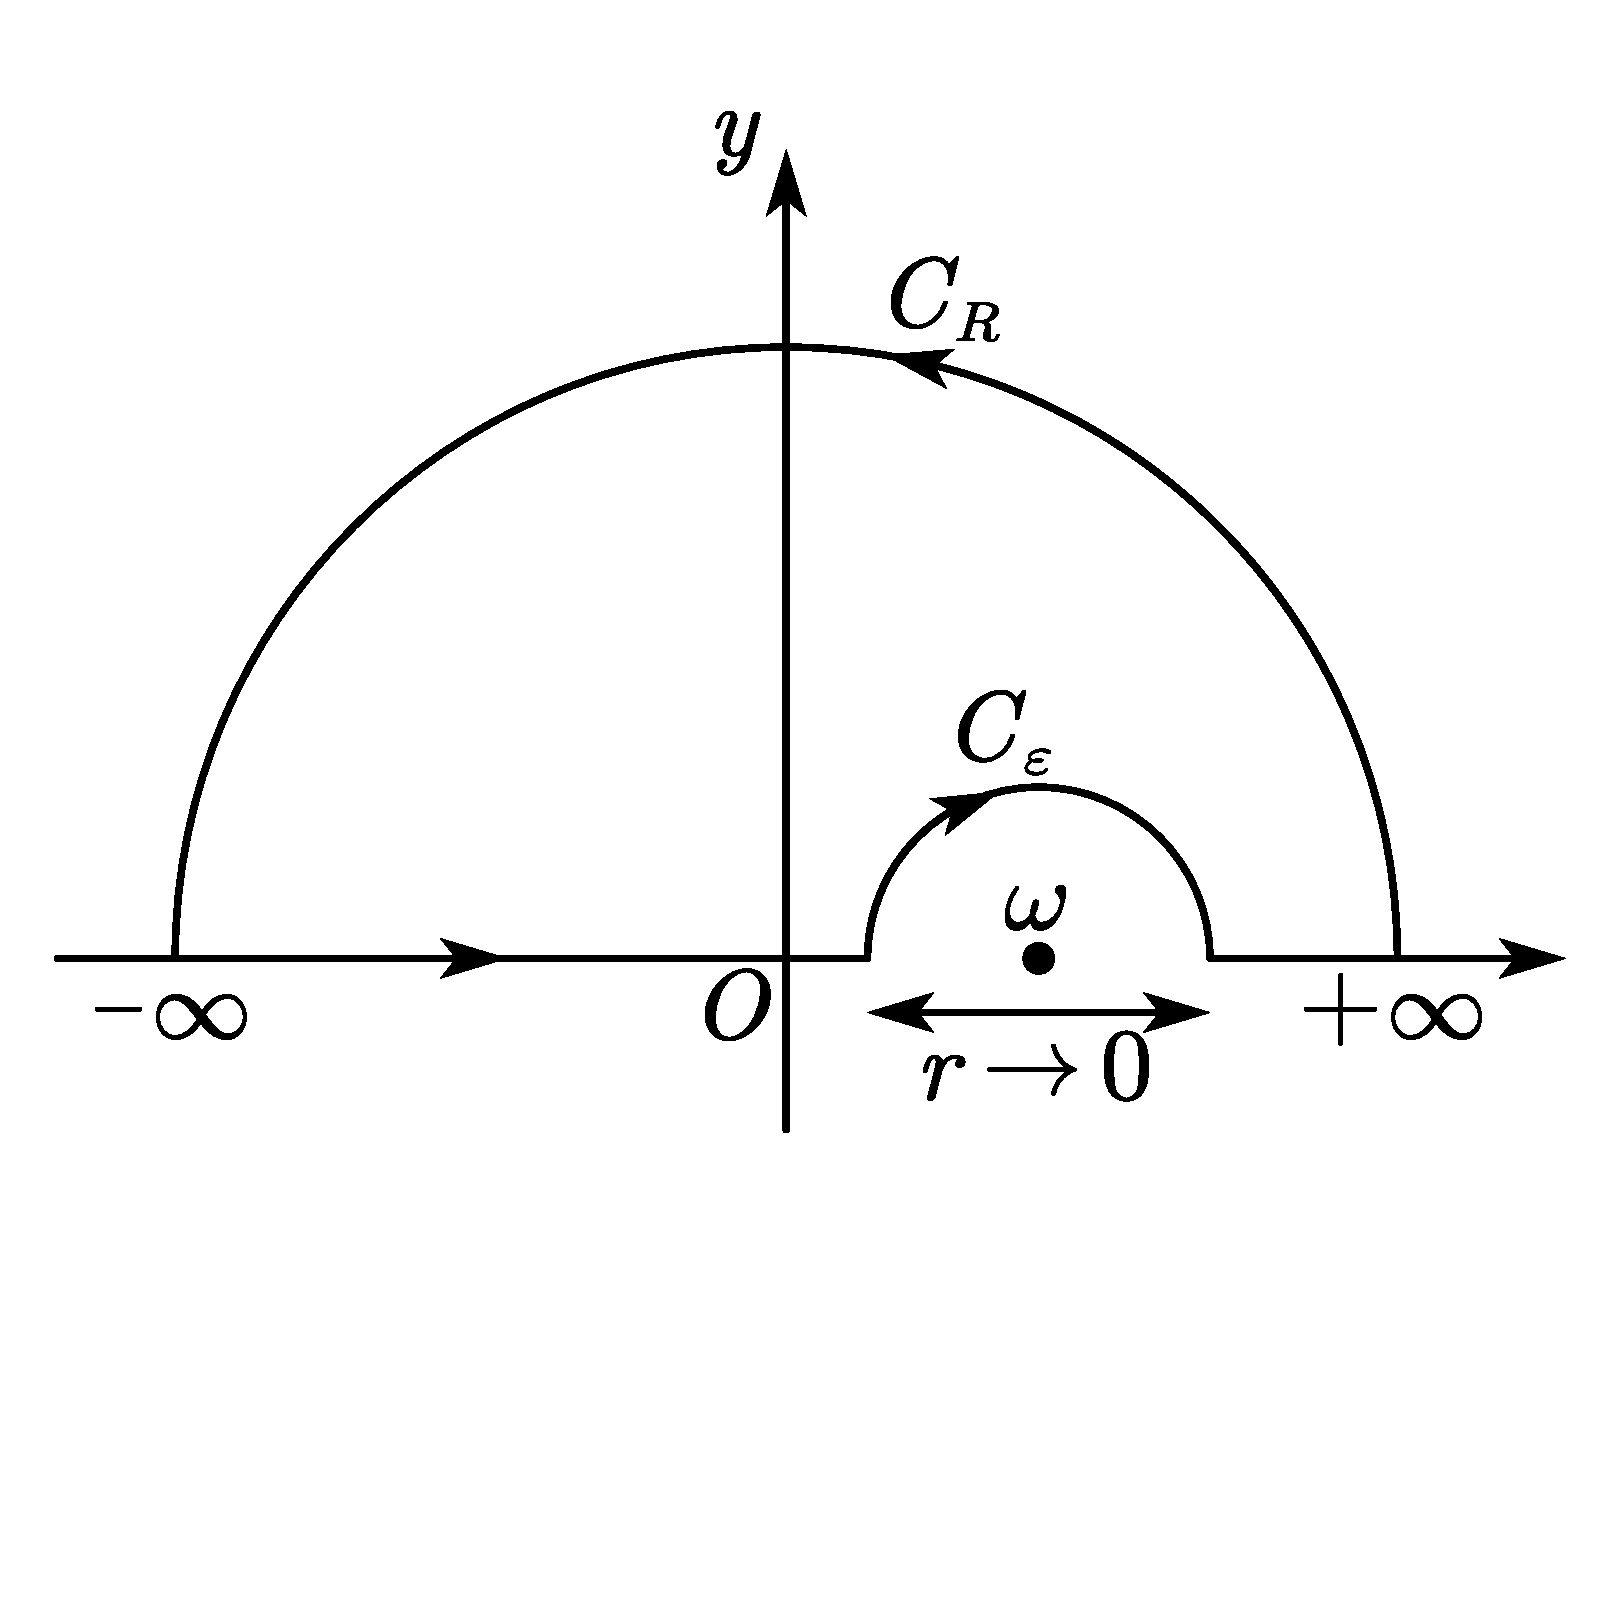
\includegraphics[width=7cm]{figure/k-k-relation.pdf}
        \caption{上半平面的围道积分}
        \end{figure}
     考虑如图的回路积分, 积分回路不包含实轴上的奇点, 所以如果函数是解析的, 积分应当等于零. 根据上面的分析, 推迟格林函数在上半复平面上解析, 且在无穷远处渐近地趋于零, 所以有
     \begin{equation}
         \oint \frac{G_{AB}^{\mathrm{R}}(z)}{z-\omega}\dd z=0,
     \end{equation}
回路积分可以分成三部分:
     \begin{equation}
        \left\{
            \begin{aligned}
                &\mbox{沿大圆积分}=0,\\
                &\mbox{沿实轴积分}=\mathcal{P}\int_{-\infty}^{\infty}\frac{G_{AB}^{\mathrm{R}}(\omega')}{\omega'-\omega}\dd\omega',\\
                &\mbox{沿小圆积分(由留数定理)}=-\mathrm{i}\pi G_{AB}^{\mathrm{R}}(\omega),
            \end{aligned}
        \right.
     \end{equation}
     于是得到
     \begin{equation}
         \mathcal{P}\int_{-\infty}^{\infty}\frac{G_{AB}^{\mathrm{R}}(\omega')}{\omega'-\omega}\dd\omega'-\mathrm{i}\pi G_{AB}^{\mathrm{R}}(\omega)=0.\label{k-k-relation1}
     \end{equation}
     如果把推迟格林函数拆分成实部和虚部两部分, 即
     \begin{equation}
         G_{AB}^{\mathrm{R}}(\omega)=\mathrm{Re}G_{AB}^{\mathrm{R}}(\omega)+\mathrm{i}\mathrm{Im}G_{AB}^{\mathrm{R}}(\omega),
     \end{equation}
    对比式中的实部和虚部, 就得到了推迟格林函数的 Kramers-Kronig 色散关系:
    \begin{equation}
        \boxed{\left\{ \begin{aligned}
                    \mathrm{Re}G_{AB}^{\mathrm{R}}(\omega)&=\frac{1}{\pi}\int_{-\infty}^\infty\frac{\mathrm{Im}G_{AB}^{\mathrm{R}}(\omega')}{\omega'-\omega}\dd \omega',\\
                    \mathrm{Im}G_{AB}^{\mathrm{R}}(\omega)&=-\frac{1}{\pi}\int_{-\infty}^{\infty}\frac{\mathrm{Re}G_{AB}^{\mathrm{R}}(\omega')}{\omega'-\omega}\dd \omega'.
        \end{aligned}\right.}
    \end{equation}
    \begin{question}{}{}
        推导超前格林函数 $G_{AB}^{\mathrm{A}}(\omega)$ 的 Kramers-Kronig 色散关系.
    \end{question}

\section{$G_{AB}^{\mathrm{R}}(\omega)$ 的若干应用}

    (1)  $G_{AB}^{\mathrm{R}}$ 本身即为某种关联函数或者传播子. 
    
    (2)  $\langle \hat{B}\hat{A} \rangle_T$ 用 $G_{AB}^{\mathrm{R,A}}(\omega)$ 表示 (谱定理).
    
    由谱函数表达式出发,
        \begin{align}
            A(\omega)&=\frac{1}{\mathcal{Z}}\sum_m\sum_n\mathrm{e}^{-\beta E_m}\left( \mathrm{e}^{-\beta(E_n-E_m)}+\epsilon \right) B_{mn}A_{nm}\delta(E_m-E_n-\omega)\nonumber\\
            &=\frac{1}{\mathcal{Z}}\sum_m\sum_n\mathrm{e}^{-\beta E_m}\left( \mathrm{e}^{\beta\omega}+\epsilon \right) B_{mn}A_{nm}\delta(E_m-E_n-\omega),
        \end{align}
    然后考虑下面的函数:
 \begin{align}\label{average1}
            \int_{-\infty}^{\infty}\frac{A(\omega')}{\mathrm{e}^{\beta\omega'}+\epsilon}\dd\omega'&=\int_{-\infty}^{\infty}\frac{1}{\mathcal{Z}}\sum_m\sum_n\mathrm{e}^{-\beta E_m}B_{mn}A_{nm}\delta(E_m-E_n-\omega')\dd\omega'\nonumber\\
            &=\frac{1}{\mathcal{Z}}\sum_m\sum_n\mathrm{e}^{-\beta E_m}B_{mn}A_{nm}\nonumber\\
            &=\sum_m\sum_n\left\langle m \left| \frac{\mathrm{e}^{-\beta E_m}}{\mathcal{Z}}\hat B \right| n \right\rangle \langle n|\hat A |m \rangle\nonumber\\
            &=\sum_m\left\langle m\left| \frac{\mathrm{e}^{-\beta E_m}}{\mathcal{Z}}\hat B\hat A \right|m \right\rangle\nonumber\\
            &=\mathrm{Tr}\left[ \frac{\mathrm{e}^{-\beta E_m}}{\mathcal{Z}}\hat B\hat A \right]\nonumber\\
            &=\left\langle \hat B\hat A \right\rangle_T,
        \end{align}
这样就得到了用谱函数计算任意两算符关联函数的表达式, 这一关系式也经常被称为\textbf{谱定理}, 即:
\begin{equation}\label{eq242}
\boxed{
\left\langle \hat B\hat A \right\rangle_T=\int_{-\infty}^{\infty}\frac{A(\omega')}{\mathrm{e}^{\beta\omega'}+\epsilon}\dd\omega'.
}
\end{equation}
将式 \eqref{spectrum2} 带入上式, 就得到了
    \begin{equation}
        \left\langle \hat{B}\hat{A} \right\rangle_T=-\frac{1}{2\pi\mathrm{i}}\int_{-\infty}^{\infty}\frac{G_{AB}^{\mathrm{R}}(\omega')-G_{BA}^{\mathrm{A}}(\omega')}{\mathrm{e}^{\beta\omega'}+\epsilon}\dd\omega'.
    \end{equation}

    (3)  $G_{AB}^{\mathrm{R}}(\omega)$ 与多体系统激发谱之间的关系.
    \begin{equation}
        \begin{aligned}
            G_{AB}^{\mathrm{R}}(\omega)&=\int_{-\infty}^{\infty}\frac{A(\omega')}{\omega-\omega'+\mathrm{i}\eta}\dd\omega'\\
            &=\int_{-\infty}^{\infty}\frac{\mathrm{d}\omega'}{\omega-\omega'+\mathrm{i}\eta}\cdot \frac{1}{\mathcal{Z}}\sum_n\sum_m\left( \mathrm{e}^{-\beta E_n}+\epsilon \mathrm{e}^{-\beta E_m} \right) B_{mn}A_{nm} \delta(E_m-E_n-\omega')\\
            &=\frac{1}{\mathcal{Z}}\sum_m\sum_n\frac{1}{\omega-(E_m-E_n)+\mathrm{i}\eta}\left( \mathrm{e}^{-\beta E_n}+\epsilon \mathrm{e}^{-\beta E_m} \right) B_{mn}A_{nm},
        \end{aligned}\label{excite1}
    \end{equation} 
    其中, 取零温极限 $T\to 0$, $\beta\to\infty$, 只保留最大项 $m=0$ 和 $n=0$, 配分函数可以表示成
\begin{align}
            \mathcal{Z}&=\mathrm{Tr}\left[ \mathrm{e}^{-\beta \hat{H}} \right]=\sum_m \langle m|\mathrm{e}^{-\beta\hat H}|m \rangle\nonumber\\
            &=\sum_m\mathrm{e}^{-\beta E_m}=\mathrm{e}^{-\beta E_0}+\mathrm{e}^{-\beta E_1}+\cdots\nonumber\\
            &\approx \mathrm{e}^{-\beta E_0},
        \end{align}
    于是式 \eqref{excite1} 中两项分别可以写成
    \begin{equation}
        \left\{
        \begin{aligned}
            \mbox{第一项}&=\frac{1}{\mathrm{e}^{-\beta E_0}}\sum_m\frac{\mathrm{e}^{-\beta E_0}}{\omega-(E_m-E_0)+\mathrm{i}\eta}B_{m0}A_{0m},\\
            \mbox{第二项}&=\frac{\epsilon}{\mathrm{e}^{-\beta E_0}}\sum_n\frac{\mathrm{e}^{-\beta E_0}}{\omega-(E_0-E_n)+\mathrm{i}\eta}B_{0n}A_{n0},
        \end{aligned}
        \right.
    \end{equation}
    于是格林函数可以表示成
    \begin{equation}
        G_{AB}^{\mathrm{R}}(\omega)=\sum_n\left[ \frac{B_{n0}A_{0n}}{\omega-(E_n-E_0)+\mathrm{i}\eta}+\frac{\epsilon B_{0n}A_{n0}}{\omega+(E_n-E_0)+\mathrm{i}\eta} \right],
    \end{equation}
    相应地有
    \begin{equation}
        G_{AB}^{\mathrm{R}}(t)=-\mathrm{i}\theta(t)\langle 0|[\hat{A}(t),\hat{B}]_\epsilon|0 \rangle.
    \end{equation}
    
选取合适的表象, 使得矩阵元非零并给出低能激发态, 那么 $G_{AB}^{\mathrm{R}}(z)$ 的极点正的实坐标确定多体系统的激发谱.
   
    (4)  $\hat{A}\hat{B}$ 是厄米算符的情况.
     
    考虑算符的系综平均应当是实值, 有
    \begin{equation}
        \left\langle \hat{B}\hat{A} \right\rangle_T=\int_{-\infty}^{\infty}\frac{A(\omega')}{\mathrm{e}^{\beta \omega'}+\epsilon}\dd\omega',
    \end{equation} 
    等式右边 $A(\omega')$ 应当也是实量, 或者虚部积分为零, 即
    \begin{equation}
        \int_{-\infty}^{\infty}\frac{\mathrm{Im}A(\omega')}{\mathrm{e}^{\beta\omega'}+\epsilon}\dd \omega'=0.
    \end{equation}
    下面我们考虑 $A(\omega')$ 为实量的情况. 根据推迟和超前格林函数的谱表示,
    \begin{equation}
        G_{AB}^{\mathrm{R}}(\omega)=\int_{-\infty}^{\infty}\frac{A(\omega')}{\omega-\omega'+\mathrm{i}\eta}\dd\omega',\quad G_{AB}^{\mathrm{A}}(\omega)=\int_{-\infty}^{\infty}\frac{A(\omega')}{\omega-\omega'-\mathrm{i}\eta}\dd\omega',
    \end{equation}
    可以得到
    \begin{equation}
        \left[ G_{AB}^{\mathrm{R}}(\omega) \right]^*=G_{AB}^{\mathrm{A}}(\omega),
    \end{equation}
    所以两格林函数的实部和虚部之间的关系是
    \begin{equation}
        \left\{
            \begin{aligned}
                \mathrm{Re}G_{AB}^{\mathrm{R}}(\omega)&=\mathrm{Re}G_{AB}^{\mathrm{A}}(\omega),\\
                \mathrm{Im}G_{AB}^{\mathrm{R}}(\omega)&=-\mathrm{Im}G_{AB}^{\mathrm{A}}(\omega),
            \end{aligned}
        \right.
    \end{equation}
    带入谱定理式 \eqref{spectrum2}, 得到
   \begin{align}
            A(\omega)&=-\frac{1}{2\pi \mathrm{i}}\left[ G_{AB}^{\mathrm{R}}(\omega)-G_{AB}^{\mathrm{A}}(\omega) \right]\nonumber\\
            &=-\frac{1}{2\pi\mathrm{i}}\left[ G_{AB}^{\mathrm{R}}(\omega)-\left( G_{AB}^{\mathrm{R}}(\omega) \right)^* \right]\nonumber\\
            &=-\frac{1}{2\pi\mathrm{i}}\left[ \mathrm{i} 2\mathrm{Im}G_{AB}^{\mathrm{R}}(\omega) \right]\nonumber\\
            &=-\frac{1}{\pi}\mathrm{Im}G_{AB}^{\mathrm{R}}(\omega),
        \end{align}
    代回 \eqref{spectrum1} 及 \eqref{eq242}, 就得到两个十分重要的表达式
    \begin{equation}
        \boxed{G_{AB}^{\mathrm{R,A}}(\omega)=\int_{-\infty}^{\infty}\left( \mp\frac{1}{\pi} \right) \frac{\mathrm{Im} G_{AB}^{\mathrm{R,A}}(\omega')\dd \omega'}{\omega-\omega'\pm \mathrm{i}\eta},}
    \end{equation}
    以及
    \begin{equation}
        \boxed{\left\langle \hat{B}\hat{A} \right\rangle_T=\int_{-\infty}^{\infty}-\frac{1}{\pi}\frac{\mathrm{Im}G_{AB}^{\mathrm{R}}(\omega')}{\mathrm{e}^{\beta\omega'}+\epsilon}\dd\omega'.}
    \end{equation}
    \begin{note}
        特别地, 下面简单讨论一下当 $\hat{F}=\hat{B}\hat{A}$ 是厄米算符时, 在什么情况下谱函数 $A(\omega)$ 会是实数. 我们考虑以下两种情况:
        
        (i) $\hat{A}$ 和 $\hat{B}$ 都不是厄米算符, 但 $\hat{B}\hat{A}$ 是厄米算符.

        在这种情况下, 算符具有性质
        \begin{equation}
            \left( \hat{B}\hat{A} \right)^\dagger =\hat{A}^\dagger \hat{B}^\dagger =\hat{B}\hat{A},
        \end{equation}
        具有这种性质的算符对的例子有 $\hat{A}=\hat{C}_{k\sigma}$ 和 $\hat{B}=\hat{C}_{k\sigma}^\dagger$ 等. 谱函数可以表示成
        \begin{equation}
            A(\omega)=\frac{1}{\mathcal{Z}}\sum_n\sum_m\left( \mathrm{e}^{-\beta E_n}+\epsilon \mathrm{e}^{-\beta E_m} \right) B_{mn}A_{nm}\delta\left( E_m-E_n-\omega \right),
        \end{equation}
        谱函数的厄米共轭:
        \begin{equation}
            A^*(\omega)=\frac{1}{\mathcal{Z}}\sum_n\sum_m\left( \mathrm{e}^{-\beta E_n}+\epsilon \mathrm{e}^{-\beta E_m} \right) (B_{mn})^* (A_{nm})^*\delta\left( E_m-E_n-\omega \right),
        \end{equation}
        其中算符矩阵元的乘积具体表示为
        \begin{equation}
            B_{mn}A_{nm}=\langle m|\hat{B}|n \rangle\langle n|\hat{A}|m \rangle,
        \end{equation}
        以及
     \begin{align}
                (B_{mn})^* (A_{nm})^*=&\langle m|\hat{B}|n \rangle^*\langle n|\hat{A}|m \rangle^*\nonumber\\
                =&\langle n|\hat{B}^\dagger |m \rangle \langle m|\hat{A}^\dagger |n \rangle\nonumber\\
                =&\langle n|\hat{A}|m \rangle\langle m|\hat{B}|n \rangle\nonumber\\
                =&B_{mn}A_{nm}.
     \end{align}
        因此在这种情况下, 谱函数满足
        \begin{equation}
            A^*(\omega)=A(\omega)
        \end{equation}
        是实数.

        (ii) 如果算符 $\hat{A}$ 和 $\hat{B}$ 都是厄米算符, 且 $\left[ \hat{A},\hat{B} \right]=0$, 从而 $\hat{F}=\hat{B}\hat{A}$ 是厄米算符.

        此时考虑算符矩阵元的乘积, 有
        \begin{equation}
            (B_{mn})^* (A_{nm})^*=\langle n|\hat{B}|m \rangle \langle m|\hat{A}|n \rangle\ne B_{mn}A_{nm},
        \end{equation}
        因此这种情况下不满足 $\hat{A}(\omega)=\hat{A}^*(\omega)$, 谱函数不是实数.

        综上讨论, 只有当算符 $\hat{A}$ 和 $\hat{B}$ 都不是厄米算符, 但 $\hat{B}\hat{A}$ 是厄米算符时, 谱函数是实数.
    \end{note}

\section{运动方程法}
以全同自由费米子系统为例, 设系统的粒子数为 $N$, 哈密顿量是
\begin{equation}
    \hat{H}=\sum_{k\sigma}E^{}_k\hat{C}_{k\sigma}^\dagger \hat{C}_{k\sigma}^{ },
\end{equation}
下面讨论如何求解这一系统的格林函数具体形式. 

格林函数的表达式是
\begin{equation}
    G_{AB}^{\mathrm{R}}(t)=-\mathrm{i}\theta(t)\left\langle \left[ \hat{C}_{k\sigma}^{ }(t),\hat{C}_{k\sigma}^{\dagger} \right]_+ \right\rangle_T,
\end{equation}
上式对时间求导数, 有
  \begin{align}\label{motion-eq1}
        \mathrm{i}\frac{\dd}{\dd t}G^{\mathrm{R}}(t)&=\mathrm{i}\frac{\dd}{\dd t}\left\{ -\mathrm{i}\theta(t)\left\langle \left[ \hat{C}_{k\sigma}^{ }(t),\hat{C}_{k\sigma}^{\dagger} \right]_+ \right\rangle_T \right\}\nonumber\\
        &=\left( \frac{\dd}{\dd t}\theta(t) \right) \left\langle \left[ \hat{C}_{k\sigma}^{ }(t),\hat{C}_{k\sigma}^{\dagger} \right]_+ \right\rangle_T-\mathrm{i}\theta(t)\left\langle \left[ \mathrm{i}\frac{\dd}{\dd t}\hat{C}_{k\sigma}^{ }(t),\hat{C}_{k\sigma}^{\dagger} \right]_+ \right\rangle_T,
    \end{align}
其中, 阶跃函数 $\theta(t)$ 的傅里叶变换是
\begin{equation}
    \theta(t)=-\frac{1}{2\pi \mathrm{i}}\int_{-\infty}^{\infty}\frac{\mathrm{e}^{-\mathrm{i} xt}}{x+\mathrm{i}\eta}\dd x,
\end{equation}
对时间的导数就是
   \begin{align}\label{theta-fourier}
        \frac{\dd}{\dd t}\theta(t)&=-\frac{1}{2\pi\mathrm{i}}\int_{-\infty}^{\infty}\frac{(-\mathrm{i} x)\mathrm{e}^{-\mathrm{i} xt}}{x+\mathrm{i}\eta}\dd x\nonumber\\
        &=\frac{1}{2\pi}\int_{-\infty}^{\infty}\frac{x\mathrm{e}^{-\mathrm{i} xt}}{x+\mathrm{i}\eta}\dd x\nonumber\\
        &=\frac{1}{2\pi}\int_{-\infty}^{\infty}\frac{(x+\mathrm{i}\eta-\mathrm{i}\eta)\mathrm{e}^{-\mathrm{i} xt}}{x+\mathrm{i} \eta}\dd x\nonumber\\
        &=\frac{1}{2\pi}\int_{-\infty}^{\infty}\mathrm{e}^{-\mathrm{i} xt}\dd x-\frac{\mathrm{i}\eta}{2\pi}\int_{-\infty}^{\infty}\frac{\mathrm{e}^{-\mathrm{i} xt}}{x+\mathrm{i}\eta}\dd x\nonumber\\
        &=\delta(t)-\eta\theta(t),
    \end{align}
此外,式 \eqref{motion-eq1} 中第二项可以利用海森伯方程写成
  \begin{align}\label{heisenberg1}
        \mathrm{i}\frac{\dd}{\dd t}\hat{C}_{k\sigma}^{ }(t)&=\left[ \hat{C}_{k\sigma}(t),\hat{H} \right]_-\nonumber\\
        &=\left[ \mathrm{e}^{\mathrm{i}\hat{H}t}\hat{C}_{k\sigma}^{ }\mathrm{e}^{-\mathrm{i}\hat{H}t},\hat{H} \right]_-\nonumber\\
        &=\mathrm{e}^{\mathrm{i}\hat{H}t}\left[ \hat{C}_{k\sigma},\hat{H} \right]_-\mathrm{e}^{-\mathrm{i}\hat{H}t},
    \end{align}
其中, 考虑到在费米子系统中, 利用反对易式 $[\; ,\;]_+$ 计算更方便, 可以利用恒等式
\begin{equation}
    \left[ \hat{A},\hat{B}\hat{C} \right]_-=\left[ \hat{A},\hat{B} \right]_+\hat{C}-\hat{B}\left[ \hat{A},\hat{C} \right]_+,
\end{equation}
将对易式简化成
   \begin{align}
        \left[ \hat{C}_{k\sigma}^{ },\hat{H} \right]_- &=\left[ \hat{C}_{k\sigma},\sum_{k^\prime}\sum_{\sigma'}E_{k'}\hat{C}_{k^\prime\sigma'}^{\dagger} \hat{C}_{k^\prime\sigma'}^{ } \right]_-\nonumber\\
        &=\sum_{k^\prime}\sum_{\sigma'}E_{k'}\left[ \hat{C}_{k\sigma}^{ },\hat{C}_{k^\prime\sigma'}^{\dagger}\hat{C}_{k'\sigma'}^{ } \right]_-\nonumber\\
        &=\sum_{k'}\sum_{\sigma'}E_{k'}\left( \underbrace{\left[ \hat{C}_{k\sigma}^{ },\hat{C}_{k'\sigma'}^{\dagger} \right]_+}_{=\delta_{kk'}\delta_{\sigma\sigma'}} \hat{C}_{k'\sigma'}^{ }-\hat{C}_{k'\sigma'}^{\dagger}\underbrace{\left[ \hat{C}_{k\sigma}^{ },\hat{C}_{k'\sigma'}^{ } \right]_+}_{=0} \right)\nonumber\\
        &=\sum_{k'}\sum_{\sigma'}E_{k'}\delta_{kk'}\delta_{\sigma\sigma'}\hat{C}_{k'\sigma'}^{ }\nonumber\\
        &=E^{}_{k}\hat{C}_{k\sigma}^{ }.
    \end{align}
代回海森伯方程 \eqref{heisenberg1}, 得到
\begin{equation}
    \mathrm{i}\frac{\dd}{\dd t}\hat{C}_{k\sigma}(t)=E_k\hat{C}_{k\sigma}(t),\label{heisenberg2}
\end{equation}
将 \eqref{theta-fourier} 的结果和式 \eqref{heisenberg1} 带入格林函数对时间的导数 \eqref{motion-eq1}, 有
  \begin{align}
        \mathrm{i}\frac{\dd}{\dd t}G^{\mathrm{R}}(t)&=\left( \delta(t)-\eta\theta(t) \right)\left\langle \left[ \hat{C}_{k\sigma}^{ }(t),\hat{C}_{k\sigma}^{\dagger} \right]_+ \right\rangle_T-\mathrm{i}\theta(t)\left\langle \left[ E_k\hat{C}_{k\sigma}^{ }(t),\hat{C}_{k\sigma}^{\dagger} \right]_+ \right\rangle_T\nonumber\\
        &=\delta(t)\underbrace{\left\langle \left[ \hat{C}_{k\sigma}^{ },\hat{C}_{k\sigma}^{\dagger} \right]_+ \right\rangle_T}_{=1}-\mathrm{i}\eta G^{\mathrm{R}}(t)+E_kG^{\mathrm{R}}(t)\nonumber\\
        &=\delta(t)-\mathrm{i}\eta G^{\mathrm{R}}(t)+E_kG^{\mathrm{R}}(t),
    \end{align}
这样就得到了自由费米子系统的格林函数运动方程, 即
\begin{equation}
    \mathrm{i}\frac{\dd}{\dd t}G^{\mathrm{R}}(t)=\delta(t)-\mathrm{i}\eta G^{\mathrm{R}}(t)+E_kG^{\mathrm{R}}(t).\label{motion-eq2}
\end{equation}

如果考虑傅里叶变换
\begin{equation}
    \left\{\begin{aligned}
        G^{\mathrm{R}}(t)&=\frac{1}{2\pi}\int_{-\infty}^{\infty}G^{\mathrm{R}}(\omega)\mathrm{e}^{-\mathrm{i}\omega t}\dd \omega,\\
        \delta(t)&=\frac{1}{2\pi}\int_{-\infty}^{\infty}\mathrm{e}^{-\mathrm{i}\omega t}\dd \omega,
    \end{aligned}\right.
\end{equation}
带入式 \eqref{motion-eq2}, 就得到了
 \begin{align}
        \omega G^{\mathrm{R}}(\omega)&=-\mathrm{i}\eta G^{\mathrm{R}}(\omega)+E_k G^{\mathrm{R}}(\omega)+1\nonumber\\
        \Rightarrow G^{\mathrm{R}}(\omega)&=\frac{1}{\omega-E_k+\mathrm{i}\eta},
    \end{align}
于是谱函数可以表示成
\begin{equation}
    A(\omega)=-\frac{1}{\pi}\mathrm{Im}G^{\mathrm{R}}(\omega)=\delta(\omega-E_k).
\end{equation}

另外, 根据式 \eqref{average1}, 系统的粒子数密度平均值可以表示成
\begin{equation}
    \langle \hat{n}_{k\sigma} \rangle_T=\int\frac{\delta(\omega'-E_k)}{\mathrm{e}^{\beta\omega'}+1}\dd\omega'=\frac{1}{\mathrm{e}^{\beta E_k}+1},
\end{equation}
此即费米分布函数. 
\begin{question}{}{}
自由费米子系统中, 利用对易子 $[\; ,\;]_{-}$ 重新计算格林函数运动方程.
\end{question}

需要注意的是:
\begin{itemize}
\item 求系统的激发谱, 总粒子数不变, 选择的算符 $\hat A$ 和 $\hat B$ 也必须保持粒子数不变.
\item 对于有限温度下全同费米子系统或全同玻色子系统的一些量子统计, 考虑巨正则系综非常方便. 正则系综也能算出来, 但更复杂.
\end{itemize}

下面计算粒子态密度. 考虑巨正则系综, 总粒子数可以表示为:
\begin{align}
N= &\langle\hat{N}\rangle_{\mu}=\left\langle\sum_{k  \sigma} \hat{n}_{k  \sigma}\right\rangle_{\mu}=\sum_{k  \sigma}\left\langle\hat{n}_{k  \sigma}\right\rangle_{\mu} \nonumber\\
=&\sum_{k  \sigma} \int_{-\infty}^{\infty} \frac{-\frac{1}{\pi} \operatorname{Im} G^{\mathrm{R}}_{k }(\omega)}{\mathrm{e}^{\beta \omega}+1} \mathrm{d} \omega\nonumber \\
\xlongequal[]{\omega \rightarrow \omega-\mu}& \sum_{k  \sigma} \int_{-\infty}^{\infty} \frac{-\frac{1}{\pi} \operatorname{Im} G^{\mathrm{R}}_{k }(\omega-\mu)}{\mathrm{e}^{\beta(\omega-\mu)}+1} \mathrm{~d} \omega\nonumber \\
\equiv&\int_{-\infty}^{\infty} n_{\mathrm{F}}(\omega) \rho(\omega) \mathrm{d} \omega ,
\end{align}
其中 $\displaystyle n_{\mathrm{F}}(\omega)=\frac{1}{\mathrm{e}^{\beta (\omega-\mu)}+1}$ 是费米子分布概率(平均占据数). $\rho(\omega)$ 就是粒子态密度, 也称为态密度, 具体表达式为:
\begin{equation}
\rho(\omega) =\sum_{k  \sigma}\left[-\frac{1}{\pi} \operatorname{Im} G^{\mathrm{R}}_{k }(\omega-\mu)\right] .
\end{equation}
虽然这个结果是用无相互作用系统推出的, 但其是普适的. 对于有相互作用系统, 只需要将 $G^{\mathrm{R}}_{k }$ 替换为有相互作用的格林函数即可.

回到无相互作用系统, 在三维情况下 
\begin{equation}
\rho(\omega) =\sum_{k  \sigma} \delta\left(\omega-E_{k}^0 \right)\propto \sqrt{\omega}.
\end{equation}

\begin{question}{}{}
已知相互作用系统的哈密顿量
\begin{equation}
\hat{H}=\sum_{k  \sigma} (E_{k}^{(1)}-\mu) \hat{a}_{k  \sigma}^{\dagger} \hat{a}_{k  \sigma}^{}+\sum_{k  \sigma} (E_{k}^{(2)}-\mu) \hat{b}_{k  \sigma}^{\dagger} \hat{b}_{k  \sigma}^{}+V\sum_{k  \sigma} \left(\hat{a}_{k  \sigma}^{\dagger} \hat{b}_{k  \sigma}^{}+\hat{b}_{k  \sigma}^{\dagger} \hat{a}_{k  \sigma}^{}\right),
\end{equation}
分别计算 $a$ 带和 $b$ 带的粒子态密度.
\end{question}

\section{格林函数方法的实际应用}
\subsection{对铁磁海森伯模型的应用}
在固体中, 处于格点上的原子核和电子都带有自旋, 因此每个格点上会呈现出磁矩. 磁矩不为零的格点称为磁性格点. 多数情况下, 不同磁性格点上磁矩的取向不同. 当有外磁场时, 磁矩倾向于平行外磁场排列. 但某些铁磁体物质(如铁, 钴, 镍等)在温度不太高时, 即使无外磁场, 每个磁性格点上磁矩也会平行排列, 在宏观上表现出磁化强度, 这种情况称为自发磁化. 有的物质在自发磁化时, 相邻磁性格点上的磁矩取向相反, 这种物质称为反铁磁体.
如果相邻磁性格点的磁矩取向相反, 但大小不等, 则称为亚铁磁体. 

铁磁性是一种量子力学效应, 由于电子的全同性, 两个电子体系的波函数必须反对称. 如果两电子自旋同向(自旋波函数对称), 则其轨道波函数反对称; 如果自旋反向, 轨道波函数应该对称. 由波函数的对称性, 造成两个电子间库仑作用的一种特殊贡献, 称为交换能, 以下记作 $J$. 这一物理量与两电子的自旋状态有关. 下面具体讨论铁磁海森伯模型的应用.
\subsubsection{海森伯模型}
海森伯模型是描述量子磁性的基本模型, 这一模型同时可以很好地描述一些由量子自旋算符带来的效应. 通过研究海森伯模型的基态, 激发态和热力学相, 人们得到了很多重要的物理概念和技术. 该模型由海森伯于1928年提出, 后来Dirac于1929年给出自旋为 $1 / 2$ 时该模型哈密顿量的证明, 1963年Anderson证明了自旋大于 $1 / 2$ 时的海森伯模型. 


海森伯模型的哈密顿量为:
\begin{equation}
\hat{H}=-{\sum_{ll^{\prime}}}^{\prime} J_{l l^{\prime}} \hat{\boldsymbol{S}}_{l} \cdot \hat{\boldsymbol{S}}_{l^{\prime}},
\end{equation}
其中 $\displaystyle{\sum_{ll^{\prime}}}^{\prime}$ 表示对 $l\neq l'$ 的全部格点求和, $\hat{\boldsymbol{S}}_{l}$ 表示第 $l$ 个格点的自旋算符. $J_{l l^{\prime}}$ 从泡利不相容原理来, 是交换积分. 当$J_{l l^{\prime}}>0$ 时可以描述铁磁体, $J_{l l^{\prime}}<0$ 时可以描述反铁磁体. 下面给出几个常见的“海森伯”模型.

设哈密顿量为:
\begin{equation}
\hat{H}=-{\sum_{ll^{\prime}}}^{\prime} J_{l l^{\prime}}\left[\alpha\left(\hat{S}_{l}^{x} \hat{S}_{l^{\prime}}^{x}+\hat{S}_{l}^{y} \hat{S}_{l^{\prime}}^{y}\right)+\beta \hat{S}_{l}^{z} \hat{S}_{l^{\prime}}^{z}\right],
\end{equation}
其中 $\alpha\left(\hat{S}_{l}^{x} \hat{S}_{l^{\prime}}^{x}+\hat{S}_{l}^{y} \hat{S}_{l^{\prime}}^{y}\right)$ 是横向部分, $\beta \hat{S}_{l}^{z} \hat{S}_{l^{\prime}}^{z}$ 是纵向部分, 两部分在自旋动力学中作用不同. 有如下几种情况: 
\begin{itemize}
\item $\alpha=\beta=1$, 海森伯模型——无严格解; 
\item $\alpha=1, \beta=0$,  X-Y 模型——部分(低维)有严格解;
\item $\alpha=0, \beta=1$, Ising 模型——部分(低维)有严格解.
\end{itemize}
对于海森伯模型, 如果
\begin{equation}
\alpha=\beta=1, J_{l l^{\prime}}=J \delta_{l^{\prime}, l+\rho},
\end{equation}
其中 $\rho$ 表示最近邻格点的矢差, 这时的模型称为各向同性紧束缚海森伯模型. 下面我们主要讨论该模型, 其哈密顿量为:
\begin{equation}
\hat{H}=-J \sum_{l} \sum_{\rho} \hat{\boldsymbol{S}}_{l} \cdot \hat{\boldsymbol{S}}_{l+\rho}.
\end{equation}

在进一步讨论这个模型前, 我们先回顾一下有关自旋算符的内容:
\begin{itemize}
\item 自旋算符间的对易关系
\begin{equation}
\left[\hat{S}_{l}^{\alpha}, \hat{S}_{l^{\prime}}^{\beta}\right]_{-}=\mathrm{i} \varepsilon_{\alpha \beta \gamma} \hat{S}_{l}^{\gamma} \delta_{l l^{\prime}}, \quad \alpha, \beta, \gamma=x, y, z.
\end{equation}

\item 升降算符
\begin{equation}
\hat{S}_{l}^{\pm}=\hat{S}_{l}^{x} \pm \mathrm{i} \hat{S}_{l}^{y},
\end{equation}
满足对易式
\begin{equation}\label{sjsfdy}
\left[\hat{S}_{l}^{\pm}, \hat{S}_{l^{\prime}}^{z}\right]_{-}=\mp \hat{S}_{l}^{\pm} \delta_{l l^{\prime}}, \quad\left[\hat{S}_{l}^{+}, \hat{S}_{l^{\prime}}^{-}\right]_{-}=2 \hat{S}_{l}^{z} \delta_{l l^{\prime}}.
\end{equation}

\item $\hat{S}_{l}^{2}$ 和 $\hat{S}_{l}^{z}$的共同本征态 $|S, m\rangle_{l}$
\begin{align}
\hat{S}_{l}^{2}|S, m\rangle_{l}&=S(S+1)|S, m\rangle_{l} , \nonumber\\
\hat{S}_{l}^{z}|S, m\rangle_{l}&=m|S, m\rangle_{l} , \nonumber\\
\hat{S}_{l}^{+}|S, m\rangle_{l}&=\sqrt{(S-m)(S+m+1)}|S, m+1\rangle_{l} ,\nonumber \\
\hat{S}_{l}^{-}|S, m\rangle_{l}&=\sqrt{(S+m)(S-m+1)}|S, m-1\rangle_{l} .
\end{align}
其中 $m=-S,-S+1,\cdots,S$, 且有
\begin{equation}
\hat{S}_{l}^{+}|S, m=S\rangle_{l}=0, \quad \hat{S}_{l}^{-}|S,m=-S\rangle_{l}=0.
\end{equation}
对于含有 $N$ 个格点的体系, 体系自旋空间的维数(本征态的个数)将是 $(2 S+1)^{N}$.
\end{itemize}

\subsubsection{铁磁海森伯模型的若干理论结果}
考虑各向同性的铁磁海森伯模型, 其哈密顿量为:
\begin{align}
\hat{H} &=-J \sum_{l} \sum_{\rho} \hat{\boldsymbol{S}}_l \cdot \hat{\boldsymbol{S}}_{l+\rho}\nonumber \\
&=-J \sum_{l} \sum_{\rho}\left[\hat{S}_{l}^{z} \hat{S}_{l+\rho}^{z}+\frac{1}{2}\left(\hat{S}_{l}^{+} \hat{S}_{l+\rho}^{-}+\hat{S}_{l}^{-} \hat{S}_{l+\rho}^{+}\right)\right] \nonumber\\
&=-J \sum_{l} \sum_{\rho}\left(\hat{S}_{l}^{z} \hat{S}_{l+\rho}^{z}+\hat{S}_{l}^{-} \hat{S}_{l+\rho}^{+}\right) .
\end{align}
对于铁磁海森伯模型, $J>0$. 上式最后一行利用了不同格点间算符的对易关系\eqref{sjsfdy}, 同时考虑到求和是对全体格点进行的. 下面简单讨论一下铁磁海森伯模型的基态和激发态.

(a) 基态、激发态

1. 基态

直接考虑能量的基态并不容易, 通常我们寻找与哈密顿量对易的算符, 求得共同本征态, 进而确定能量本征态. 这里我们可以考虑总自旋算符和沿 $z$ 方向的总自旋算符:
\begin{equation}
\hat{\boldsymbol{S}}_{\mathrm{tot}}=\sum_{l} \hat{\boldsymbol{S}}_{l}, \quad \hat{S}_{\mathrm{tot}}^{z}=\sum_{l} \hat{S}_{l}^{z} .
\end{equation}
注意到:
\begin{align} 
{\left[\sum_{l, \rho} \hat{S}_{l}^{-} \hat{S}_{l+\rho}^{+}, \sum_{l^{\prime}} \hat{S}_{l^{\prime}}^{z}\right]_{-} } 
&=\sum_{l, \rho} \sum_{l^{\prime}}\left[\hat{S}_{l}^{-} \hat{S}_{l+\rho}^{+}, \hat{S}_{l^{\prime}}^{z}\right]_{-} \nonumber\\ 
&=\sum_{l, \rho} \sum_{l^{\prime}}\left(\hat{S}_{l}^{-}\left[\hat{S}_{l+\rho}^{+}, \hat{S}_{l^{\prime}}^{z}\right]_{-}+\left[\hat{S}_{l}^{-}, \hat{S}_{l^{\prime}}^{z} \right]_{-}\hat{S}_{l+\rho}^{+}\right)\nonumber\\ 
&=\sum_{l, \rho} \sum_{l^{\prime}}\left(-\hat{S}_{l}^{-} \hat{S}_{l^{\prime}}^{+} \delta_{l+\rho,l^{\prime}}+\hat{S}_{l^{\prime}}^{-} \hat{S}_{l+\rho}^{+} \delta_{l l^{\prime}}\right)\nonumber \\ 
&=0 ,
\end{align}
可以得到: 
\begin{equation}
\left[\hat{H}, \hat{S}_{\text {tot }}^{z}\right]_{-}=0. 
\end{equation}
所以 $\hat{H}$ 和 $\hat{S}_{\text {tot }}^{z}$ 有共同本征态, 利用前面给出的 $\hat{S}_{l}^{2}$ 和 $\hat{S}_{l}^{z}$ 的共同本征态, 可以得到体系的本征态为: $\displaystyle\prod_{l}|S, m\rangle_{l}$, 可以预期体系的基态是自旋全部同向排列, 即 $\displaystyle\prod_{l}|S, S\rangle_{l}$:
\begin{equation}
\hat{S}_{\text{tot}}^{z} \prod_{l}|S, S\rangle_{l}=N S \prod_{l}|S, S\rangle_{l}.
\end{equation}
\begin{figure}[htbp]
    \centering
    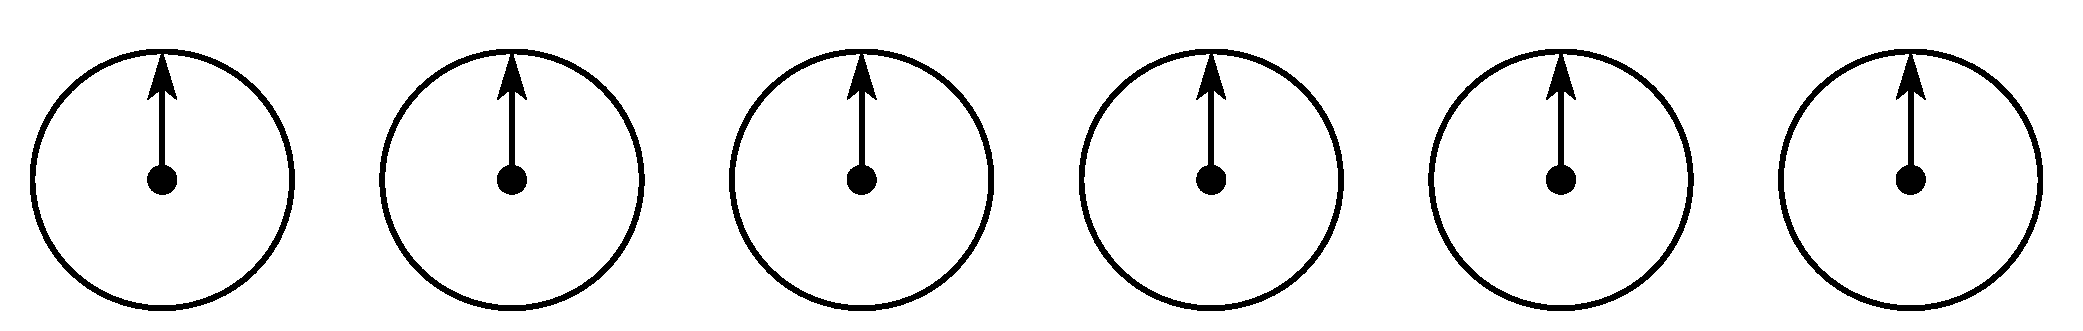
\includegraphics[width=10cm]{figure/ground-state.pdf}
    \caption{铁磁海森伯模型的基态.}
\end{figure}
\\将 $\displaystyle\prod_{l}|S, S\rangle_{l}$ 记为 $|g\rangle$, 可以证明 $|g\rangle$ 也是哈密顿算符 $\hat{H}$ 的本征态, 对应的本征值为 $E_g$:
\begin{equation}\label{HW7}
\hat{H}|g\rangle=E_{g}|g\rangle=-J S^{2} N Z |g\rangle,
\end{equation}
其中 $Z$ 为配位数.
\begin{question}{}{}
证明式\eqref{HW7}.
\end{question}

2. 自旋缺陷态

考虑某一个格点上的自旋偏转, 此时相当于基态模型在某一个格矢 $\boldsymbol{l}$ 所标记的格点上产生了一个自旋缺陷.
\begin{figure}[htbp]
    \centering
    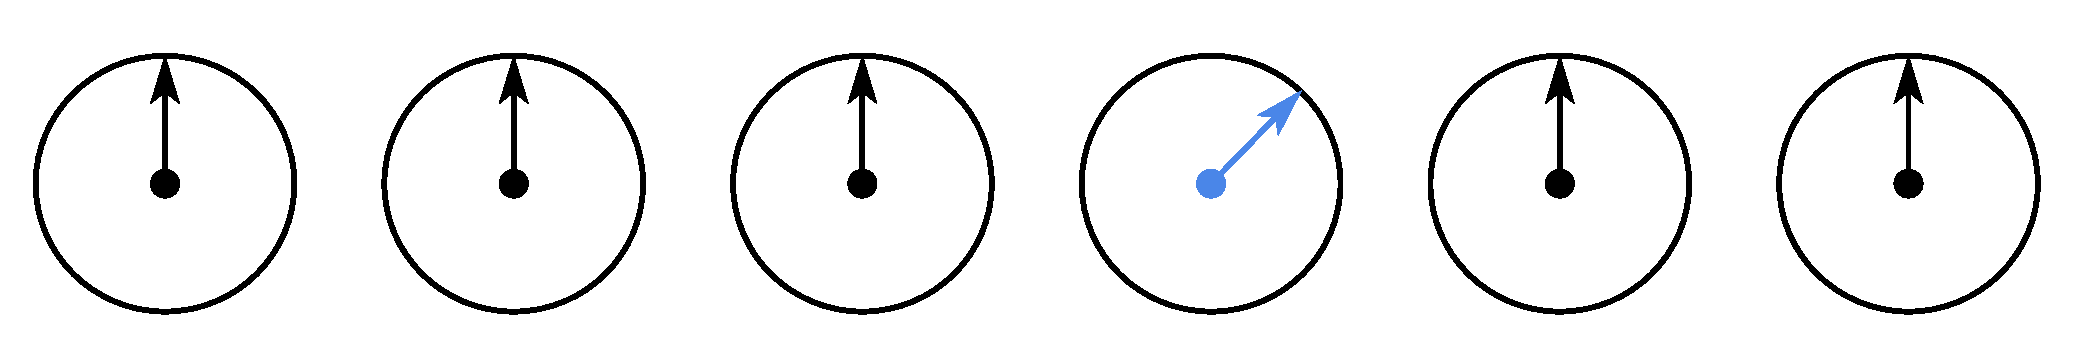
\includegraphics[width=10cm]{figure/excite-state.pdf}
    \caption{铁磁海森伯模型的自旋缺陷态.}
\end{figure}
\\ 记这一自旋缺陷态为 $|\boldsymbol{l}\rangle$, 满足
\begin{equation}
|\boldsymbol{l}\rangle \propto \hat{S}_{l}^{-}|g\rangle.
\end{equation}
可以证明, 归一化后的自旋缺陷态是
\begin{equation}
|\boldsymbol{l}\rangle = \frac{1}{\sqrt{2S}}\hat{S}_{l}^{-}|g\rangle.
\end{equation}
\begin{proof}
    设自旋缺陷态为
    \begin{equation}
        |\boldsymbol{l}\rangle=C\hat{S}_l^-|g\rangle,
    \end{equation}
    其中 $C$ 是待定常系数. 由归一化条件 $\langle l|l \rangle=\mathbbm{1}$, 得到
    \begin{equation}
        \begin{aligned}
            \left\langle g \left|\left( \hat{S}_l^- \right)^\dagger \hat{S}_l^- \right| g \right\rangle |C|^2=&\left(\sqrt{2S}\right)^2 |C|^2\\
            =&2S|C|^2=1,
        \end{aligned}
    \end{equation}
    从而 $C=1/\sqrt{2S}$. 故有
    \begin{equation}
        |\boldsymbol{l}\rangle = \frac{1}{\sqrt{2S}}\hat{S}_{l}^{-}|g\rangle.
        \end{equation}
\end{proof}

自选缺陷态具有性质
\begin{equation}
\hat{S}_{\text{tot}}^{z}|\boldsymbol{l}\rangle=(N S-1) |\boldsymbol{l}\rangle.
\end{equation}

\begin{question}{}{}
证明 $|\boldsymbol{l}\rangle$ 不是 $\hat{H}$ 本征态.
\end{question}

3. 低能激发态

可用 $N$ 个简并态的线性组合构造 $\hat{H}$ 和 $\hat{S}_{\text{tot}}^{z}$ 的共同本征态:
\begin{equation}
|\boldsymbol{k}\rangle=\frac{1}{\sqrt{2 S N}} \sum_{l} \mathrm{e}^{\mathrm{i} \boldsymbol{k} \cdot \boldsymbol{l}} \hat{S}_{l}^{-}|g\rangle,
\end{equation}
其中波矢 $\boldsymbol{k}$ 在第一布里渊区内. $|\boldsymbol{k}\rangle$ 叫做\textbf{自旋波态}, 本征方程为:
\begin{equation}
\hat{H}|\boldsymbol k \rangle=E_{k}|\boldsymbol{k}\rangle,
\end{equation}
其中
\begin{equation}\label{2821}
E_{k}=E_{g}+\omega_{k},\quad\omega_{k} \equiv 2 J Z S\left(1-\gamma_{k}\right),
\end{equation}
$\gamma_{k}$ 为结构因子: 
\begin{equation}
\gamma_{k} \equiv \frac{1}{Z} \sum_{\rho} \mathrm{e}^{\mathrm{i} \boldsymbol{k} \cdot \boldsymbol{\rho}}.
\end{equation}
对于三种立方晶格, 结构常数 $\gamma_{k}$ 的取值 (取 $a$ 为晶格常量):
\begin{equation}
\gamma_{k}= \left\{\begin{aligned}
&\displaystyle\frac{1}{3}\left[\cos \left(a k_{x}\right)+\cos \left(a k_{y}\right)+\cos\left( a k_{z}\right)\right] & \text {(简单立方,SC)}, \\ 
&\displaystyle\cos \left(\frac{1}{2} a k_{x}\right) \cos \left(\frac{1}{2} a k_{y}\right) \cos \left(\frac{1}{2} a k_{z}\right) & \text {(体心立方,BCC)}, \\ 
&\displaystyle\frac{1}{3}\left[\cos\left( \frac{1}{2} a k_{x}\right) \cos\left( \frac{1}{2} a k_{y}\right)+\cos \left(\frac{1}{2} a k_{y}\right) \cos \left(\frac{1}{2} a k_{z}\right)\right. &\\
&\displaystyle\qquad\left. +\cos \left(\frac{1}{2} a k_{z} \right)\cos \left(\frac{1}{2} a k_{x}\right)\right] & \text {(面心立方,FCC)}.\end{aligned}\right.
\end{equation}
考虑 $k \rightarrow 0$ 时的渐进性质, 有:
\begin{equation}
\lim_{k\to 0}\gamma_{k}= \left\{\begin{aligned}
\displaystyle 1-\frac{a^2 k^2}{6} \quad& \text {(简单立方,SC)}, \\ 
\displaystyle 1-\frac{a^2 k^2}{8}\quad& \text {(体心立方,BCC)}, \\ 
\displaystyle 1-\frac{a^2 k^2}{12}\quad& \text {(面心立方,FCC)}.\end{aligned}\right.
\end{equation}
对三种晶格, 均有
\begin{equation}
\lim _{k \rightarrow 0} \omega_{k} \propto k^{2} ,
\end{equation}
在此极限下, 系统无限接近基态, 故称 $|\boldsymbol{k}\rangle$ 为\textbf{低能激发态}.

(b) 铁磁自旋波理论

铁磁自旋波理论只能描述低温区 $T\ll T_\mathrm{C}$.

哈密顿量为:
\begin{equation}
\hat{H}=-J \sum_{l} \sum_{\rho} \hat{\boldsymbol{S}}_{l} \cdot \hat{\boldsymbol{S}}_{l+\rho} \quad(J>0).
\end{equation}
做Holstein-Primakoff变换(H-P变换): 
\begin{equation}
\left\{\begin{aligned}
\hat{S}_{l}^{+}&=\sqrt{2 S-\hat{a}^{\dagger}_{l} \hat{a}^{}_{l}} ~\hat{a}^{}_{l} ,\\ 
\hat{S}_{l}^{-}&=\hat{a}_{l}^{\dagger} \sqrt{2 S-\hat{a}_{l}^{\dagger} \hat{a}^{}_{l}} ,\\ 
\hat{S}_{l}^{z}&=S-\hat{a}_{l}^{\dagger} \hat{a}^{}_{l}.
\end{aligned}\right.
\end{equation}
其中引入了玻色型算符 $\hat{a}^{}_{l}, \hat{a}_{l}^{\dagger}$, 满足如下对易关系:
\begin{equation}
\left[\hat{a}_{l}^{}, \hat{a}_{l^{\prime}}^{\dagger}\right]_{-}=\delta_{l l^{\prime}}, \quad\left[\hat{a}_{l}, \hat{a}_{l^{\prime}}\right]_{-}=\left[\hat{a}_{l}^{\dagger}, \hat{a}_{l^{\prime}}^{\dagger}\right]_{-}=0.
\end{equation}
\begin{equation}
\left[\hat{S}_{l}^{\pm} ,\hat{S}_{l'}^{z} \right]_{-}=\mp\hat{S}_{l}^{\pm}\delta_{l l^{\prime}}^{},\quad
\left[\hat{S}_{l}^{+} ,\hat{S}_{l'}^{-} \right]_{-}=2\hat{S}_{l}^{z}\delta_{l l^{\prime}}^{}.
\end{equation}
再通过点阵傅里叶变换引入新的玻色算符:
\begin{equation}
\left\{\begin{aligned}
\displaystyle \hat{a}_{l}&=\frac{1}{\sqrt{N}} \sum_{ k} \mathrm{e}^{\mathrm{i} \boldsymbol {k} \cdot \boldsymbol {l}} \hat{b}_{k} ,\\
\displaystyle \hat{a}_{l}^{\dagger}&=\frac{1}{\sqrt{N}} \sum_{ k} \mathrm{e}^{-\mathrm{i} \boldsymbol {k} \cdot \boldsymbol {l}} \hat{b}_{k}^{\dagger},
\end{aligned}\right.
\end{equation}
其中 $\boldsymbol{l}=\boldsymbol{R}_{l}$ 表示正格矢. 新引入的算符同样满足玻色子的对易关系:
\begin{equation}
\left[\hat{b}^{}_{k}, \hat{b}_{k^{\prime}}^{\dagger}\right]_{-}=\delta_{k k^{\prime}}, \quad\left[\hat{b}_{k}, \hat{b}_{k^{\prime}}\right]_{-}=\left[\hat{b}_{k}^{\dagger}, \hat{b}_{k^{\prime}}^{\dagger}\right]_{-}=0.
\end{equation}
这样, 在自旋波近似下, 铁磁海森伯模型的哈密顿量可以写为自旋算符微扰展开的形式:
\begin{align}
\hat{H}=& E_{g}+\sum_{k} \omega_{k} \hat{b}_{k}^{\dagger} \hat{b}^{}_{k} \nonumber\\
&+\frac{Z J}{2 N} \sum_{k k^{\prime}} \sum_{q}\left(\gamma_{k-q}+\gamma_{k^{\prime}}-2 \gamma_{k+q-k^{\prime}}\right) \hat{b}_{k-q}^{\dagger} \hat{b}^{\dagger}_{k^{\prime}+q} \hat{b}^{}_{k^{\prime}} \hat{b}^{}_{k}+\cdots,
\end{align}
其中 $E_{g}$ 是式\eqref{HW7}中的基态能, $\omega_{k}$ 是式 \eqref{2821} 中磁振子的能量, 玻色子算符 $\hat{b}_{k}^{\dagger}$ 和 $\hat{b}^{}_{k}$ 是磁振子的产生湮灭算符. 上述哈密顿量也被称为自旋波哈密顿量, 这种处理方法就是\textbf{铁磁自旋波理论}, 在自旋波无相互作用时通常只考虑前两项, 但是处理一些非线性问题时需要考虑高阶项.

\begin{note}
    考虑自旋波态
    \begin{equation}
        |\boldsymbol{k}\rangle=\frac{1}{\sqrt{N}}\sum_l\mathrm{e}^{\mathrm{i}\boldsymbol{k}\cdot \boldsymbol{l}}|\boldsymbol{l}\rangle,
    \end{equation}
    其中
    \begin{equation}
        |\boldsymbol{l} \rangle\equiv \frac{1}{\sqrt{2S}} \hat{S}_l^-|g\rangle
    \end{equation}
    表示在第 $l$ 个格点上有自旋偏转的自旋缺陷态(已归一化). 
    下面讨论自旋波态中, 归一化系数的确定, 以及这一态函数的物理含义. 

    在自旋波态的本征方程中, 取试探解
    \begin{equation}
        |e\rangle = \sum_l C_l|\boldsymbol{l}\rangle
    \end{equation}
    代入本征方程, 得到 
   \begin{align}
            \hat{H}|e\rangle =&\sum_l C_l\hat{H}|\boldsymbol{l}\rangle\nonumber\\
            =&\sum_l C_l\left[ \left( E_g+2ZJS \right)|\boldsymbol{l}\rangle-2JS\sum_\rho |\boldsymbol{l+\rho}\rangle \right],
        \end{align}
    其中 
    \begin{align}
            \text{第二项}=&-2JS\sum_\rho\sum_l C_l|\boldsymbol{l+\rho}\rangle\nonumber\\
            =&-2JS\sum_\rho \sum_{l}C_{l-\rho} |\boldsymbol{l}\rangle ~~\quad\text{(作代换 $l+\rho\to l$)}\nonumber\\
            =&-2JS\sum_\rho f_\rho\sum_l C_l|\boldsymbol{l}\rangle,  \quad\text{(设 $C_{l-\rho}=C_lf_\rho$ 可以写成分离变量的形式)}
        \end{align}
    能够分离变量的系数最简单形式是指数函数, 即满足条件的 $C_l$ 是
    \begin{equation}
        C_l=A\mathrm{e}^{\mathrm{i}\boldsymbol{p}\cdot \boldsymbol{l}},
    \end{equation}
    从而有
    \begin{equation}
        C_{l-\rho}=A\mathrm{e}^{\mathrm{i}\boldsymbol{p}\cdot(\boldsymbol{l}-\boldsymbol{\rho})}=A\mathrm{e}^{\mathrm{i}\boldsymbol{p}\cdot \boldsymbol{l}}\cdot \mathrm{e}^{-\mathrm{i}\boldsymbol{p}\cdot \boldsymbol{\rho}},
    \end{equation}
    前面的常系数 $A$ 可以利用波恩-卡门边界条件来确定, 即
    \begin{equation}
        C_{l}=C_{l\pm a_iN_i},\quad i=1,2,3.
    \end{equation}
    $\boldsymbol{p}$ 是倒格矢, 如果限制在第一布里渊区中, 有
    \begin{equation}
        \boldsymbol{p}\Rightarrow \boldsymbol{k}=\frac{n_i\boldsymbol{b}_1}{N_i},\quad n_1=0,\pm 1,\pm 2,\cdots,
    \end{equation}
    其中 $\boldsymbol{b}_i$ 是倒点阵基矢. 倒点阵基矢和正点阵基矢之间满足
    \begin{equation}
        \boldsymbol{a}_i\cdot \boldsymbol{b}_i=2\pi\delta_{ij}.
    \end{equation}
    由归一化条件 $\langle k|k\rangle=\mathbf{1}$ 得到
    \begin{equation}
        \sum_l |A|^2\langle \boldsymbol{l}|\boldsymbol{l}\rangle=N|A|^2=\mathbf{1},
    \end{equation}
    从而定下系数 $A=1/\sqrt{N}$. 所以有归一化后的自旋波态
    \begin{equation}
        |\boldsymbol{k}\rangle=\frac{1}{\sqrt{N}}\sum_l\mathrm{e}^{\mathrm{i}\boldsymbol{k}\cdot \boldsymbol{l}}|\boldsymbol{l}\rangle.
    \end{equation}
    之所以称其为自旋波态, 是因为 $|\boldsymbol{k}\rangle$ 代表一个集体激发的态. 考虑这个态在 $z$ 方向的自旋分量, 应有 
    \begin{equation}
        \langle \boldsymbol{k}|\hat{S}_l^z |\boldsymbol{k}\rangle=S-\frac{1}{N},
    \end{equation}
    这与基态只差一个自旋量子数, 而它被 $N$ 个格点分担, 每个格点分担 $1/N$. 所以这个态应与格点指标 $l$ 无关. 引入算符 
    \begin{equation}
        \hat{S}_{k}^-\equiv \frac{1}{\sqrt{N}}\sum_l \mathrm{e}^{\mathrm{i}\boldsymbol{k}\cdot \boldsymbol{l}}\hat{S}_l^-,
    \end{equation}
    自旋波态可以改写为不带格点指标 $l$ 的形式
    \begin{equation}
        |\boldsymbol{k}\rangle=\frac{1}{\sqrt{2SN}}\sum_l\mathrm{e}^{\mathrm{i}\boldsymbol{k}\cdot \boldsymbol{l}}\hat{S}_l^-|g\rangle =\frac{1}{\sqrt{2S}}\hat{S}_{k}^-|g\rangle.
    \end{equation}
    各个格点的自旋沿 $z$ 方向的投影应当是一样的, 但在 $x-y$ 平面上的自旋方向不同. 如果把自旋箭头连起来, 就形成了一个自旋波, 这是一种集体激发.
    自旋波所对应的准粒子称为磁振子(magnon). 自旋波态的波长 $\lambda=\pi/k$. 哈密顿量的本征态可以由磁振子的量子数来确定, 自旋波态的能量就对应着磁振子的能量.      
    \begin{figure}[htbp]
        \centering
        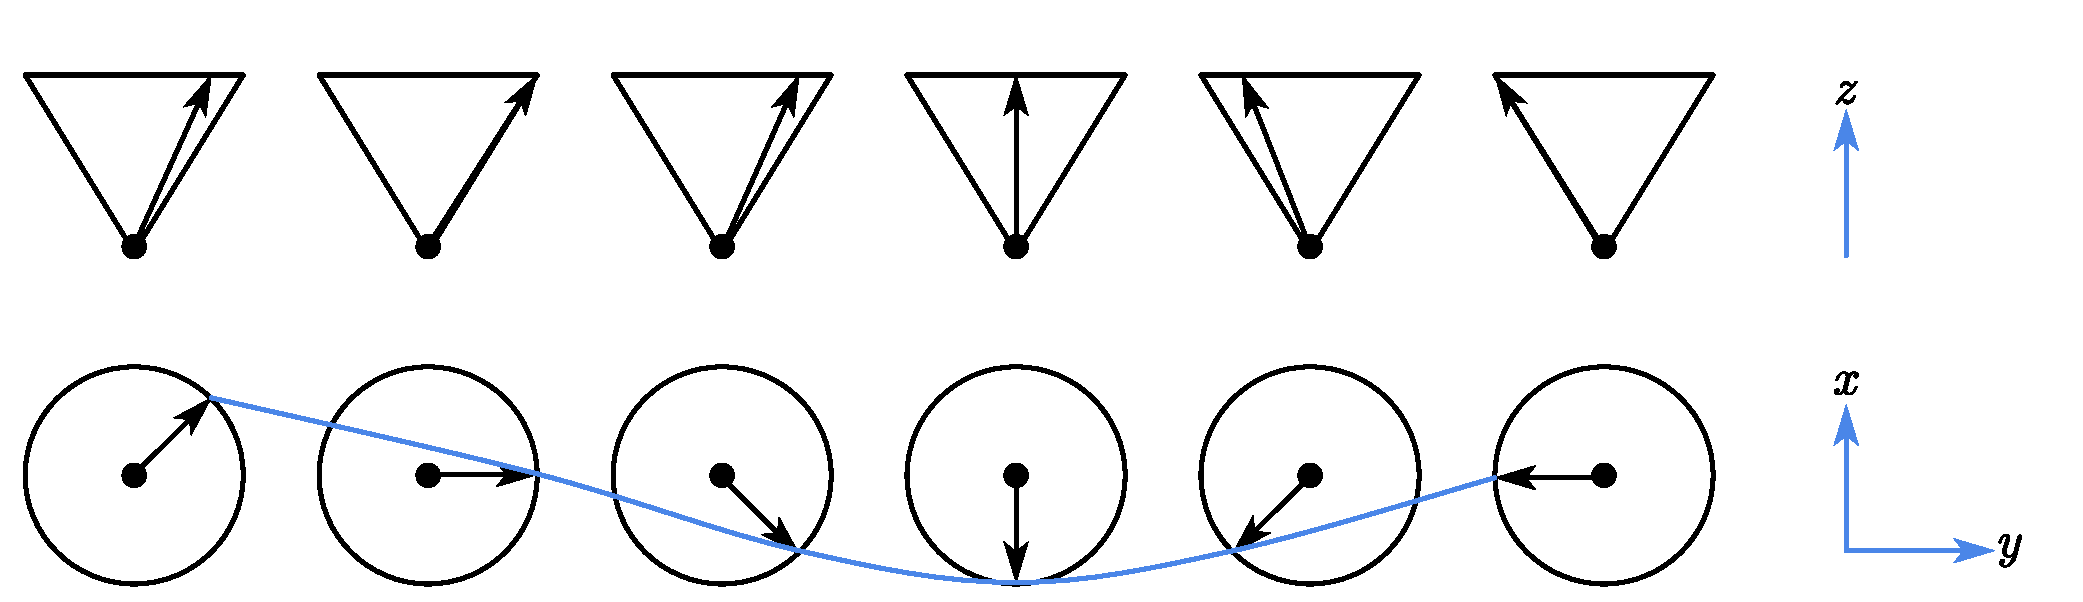
\includegraphics[width=12cm]{figure/spin-wave.pdf}
        \caption{铁磁海森伯模型的自旋波态在 $z$ 方向的投影和在 $x-y$ 平面上的自旋波.}
    \end{figure}
    
在铁磁自旋波理论中, 哈密顿量 
    \begin{equation}
        \hat{H}=E_g+\sum_{k}\omega_{k}\hat{b}_k^\dagger \hat{b}_k^{ },
    \end{equation}
    其中 $\hat{b}_k^\dagger$ 和 $\hat{b}_k^{ }$ 是磁振子的产生消灭算符. 所以应有自旋波理论的基态
    \begin{equation}
        |g\rangle\to |0\rangle,
    \end{equation}
    其中 $|0\rangle$ 代表磁振子的真空态. 这一真空态同时也是 H-P 玻色子算符的真空态, 即 
    \begin{equation}
        \hat{a}_l|0\rangle=0, \quad \hat{b}_{k}|0\rangle=0.
    \end{equation}
    此外, 还可以证明, 在 H-P 变换后, 自旋波态可以写成 
    \begin{equation}
        |\boldsymbol{k}\rangle\to \hat{b}^+_{k}|0\rangle
    \end{equation}
    的形式. 
    \begin{proof}
     \begin{align}
                |\boldsymbol{k}\rangle=&\frac{1}{\sqrt{2SN}}\sum_l\mathrm{e}^{\mathrm{i}\boldsymbol{k}\cdot \boldsymbol{l}}\hat{S}_l^-|g\rangle\nonumber\\
                =&\frac{1}{\sqrt{2SN}}\sum_l\mathrm{e}^{\mathrm{i}\boldsymbol{k}\cdot \boldsymbol{l}}\hat{a}_l^\dagger \sqrt{2S-\hat{a}^\dagger_l \hat{a}_l^{ }}|0\rangle\nonumber\\
                =&\frac{1}{\sqrt{2SN}}\sum_l\mathrm{e}^{\mathrm{i}\boldsymbol{k}\cdot \boldsymbol{l}}\hat{a}_l^\dagger \sqrt{2S}|0\rangle,
            \end{align}
        其中, 第二步到第三步按级数展开的形式理解根号下的算符, 展开式中除了零阶项 $\sqrt{2S}$ 外, 每一项都带有一个消灭算符 $\hat{a}_l$ 在最右边, 利用 $\hat{a}_l|0\rangle=0$, 就只剩下了零阶项. 再利用变换关系
        \begin{equation}
            \hat{b}^\dagger_{k}=\frac{1}{\sqrt{N}}\sum_l\mathrm{e}^{\mathrm{i}\boldsymbol{k}\cdot\boldsymbol{l}}\hat{a}_l^\dagger,
        \end{equation}
        就得到了
        \begin{equation}
            |\boldsymbol{k}\rangle=\hat{b}_{k}^\dagger |0\rangle.
        \end{equation}
    \end{proof}
\end{note}

下面简单讨论一下低温磁化率的计算. 实验中发现磁矩在低温区以 $T^{3 / 2}$ 趋近于饱和, 在临界温度处以 $\sqrt{1-T / T_\mathrm{C}}$ 趋于0(这里 $T_\mathrm{C}$ 为居里温度, 是铁磁和顺磁相变的临界温度). 先考虑总磁矩的计算, 利用H-P变换可以得到:
\begin{align}
\hat{M}^{z}_{\text{tot}} &\equiv g \mu_\mathrm{B} \sum_{l} \hat{S}_{l}^{z} \nonumber\\
&=g \mu_\mathrm{B} \sum_{l}\left(S-\hat{a}_{l}^{\dagger} \hat{a}^{}_{l}\right) \nonumber\\
&=g \mu_\mathrm{B} S N-g \mu_{B} \sum_{l} \hat{a}_{l}^{\dagger} \hat{a}^{}_{l} \nonumber\\
&=M^{z}(0)-g \mu_\mathrm{B} \sum_{k} \hat{b}_{k}^{\dagger} \hat{b}^{}_{k},
\end{align}
其中利用了
\begin{equation}
\sum_{l} \hat{a}_{l}^{\dagger} \hat{a}^{}_{l}=\sum_{k} \hat{b}_{k}^{\dagger} \hat{b}^{}_{k}.
\end{equation}
两边取均值便得到:
\begin{equation}
\left\langle\hat{M}^{z}_{\text{tot}} \right\rangle_{T}=M^{z}_{0}-g \mu_\mathrm{B} \sum_{k}\left\langle\hat{b}_{k}^{\dagger} \hat{b}_{k}^{}\right\rangle_{T}.
\end{equation}

为计算 $\displaystyle\left\langle\hat{b}_{k}^{\dagger} \hat{b}^{}_{k}\right\rangle_{T}$, 可以采用格林函数:
\begin{equation}
G_{k}^\mathrm{R}(t)=-\mathrm{i}\theta(t)\left\langle\left[\hat{b}^{}_{k}(t),\hat{b}_{k}^{\dagger}\right]_{-}\right\rangle_{T}.
\end{equation}
仿照自由电子体系的求解可以得到格林函数的傅里叶变换为:
\begin{equation}
G_{k}^\mathrm{R}(\omega)=\frac{1}{\omega-\omega_{k}+\mathrm{i} \eta},
\end{equation}
利用谱定理可以得到均值 $\left\langle\hat{b}_{k}^{\dagger} \hat{b}_{k}^{}\right\rangle_{T}$ 为:
\begin{equation}
\left\langle\hat{b}_{k}^{\dagger} \hat{b}_{k}^{}\right\rangle_{T} \equiv \int_{-\infty}^{\infty} \frac{-\frac{1}{\pi} \operatorname{Im} G_{k}^\mathrm{R}(\omega)}{\mathrm{e}^{\beta \omega}-1} \mathrm{d} \omega =\frac{1}{\mathrm{e}^{\beta \omega_{k}}-1}.
\end{equation}
这就是自由玻色子的分布函数. 

考虑到自旋波理论只适用于低能态, 类比德拜模型, 可以近似计算:
\begin{equation}\label{HW9}
\sum_{k}\left\langle\hat{b}_{k}^{\dagger} \hat{b}^{}_{k}\right\rangle_{T}\propto T^{3 / 2}.
\end{equation}
这里的 $k$ 属于第一布里渊区. 代回到磁矩均值的表达式中可以得到:
\begin{equation}
\left\langle\hat{M}^{z}(0)\right\rangle_{T}=M^{z}(0)-\alpha T^{3 / 2}.
\end{equation}
$\alpha$ 是前面的系数. 这一结果与实验上得到的结果是符合的, 由布洛赫首次得到, 因此也被称为\textbf{布洛赫 $T^{3 / 2}$ 定律}.

\begin{question}{}{}
证明关系式\eqref{HW9}.
\end{question}


需要注意的是, 虽然采用格林函数计算 $\displaystyle\left\langle\hat{b}_{k}^{\dagger} \hat{b}^{}_{k}\right\rangle_{T}$, 但其并不是格林函数方法, 而仍然是铁磁自旋波近似方法. 下面我们来介绍格林函数方法.

(c) 格林函数理论(考虑$S=1/2$)

格林函数方法适用于任何情况, 但是有时无法严格求解, 所以需要做一些近似. 回到初始时铁磁海森伯模型的哈密顿量:
\begin{equation}
\hat{H}=-J \sum_{l} \sum_{\rho}\left(\hat{S}_{l}^{z} \hat{S}_{l+\rho}^{z}+\hat{S}_{l}^{-} \hat{S}_{l+\rho}^{+}\right) ,
\end{equation}
同样 $z$ 方向的磁矩为:
\begin{equation}
M^{z}(T)=\left\langle\hat{M}^{z}\right\rangle_{T}=g \mu_\mathrm{B} \sum_{l}\left\langle\hat{S}_{l}^{z}\right\rangle_{T}.
\end{equation}
这里我们不考虑自旋波理论中的H-P变换(即不对哈密顿量做近似), 而是通过自旋算符间的关系简化上式. 考虑自旋算符的平方:
\begin{equation}
\hat{\boldsymbol{S}}_{l} \cdot \hat{\boldsymbol{S}}_{l}=\hat{S}_{l}^{z} \hat{S}_{l}^{z}+\frac{1}{2}\left(\hat{S}_{l}^{+} \hat{S}_{l}^{-}+\hat{S}_{l}^{-} \hat{S}_{l}^{+}\right),
\end{equation}
利用升降算符间的对易关系可以得到:
\begin{equation}
\left[\hat{S}_{l}^{+}, \hat{S}_{l}^{-}\right]_{-}=2 \hat{S}_{l}^{z} \Rightarrow \hat{S}_{l}^{+} \hat{S}_{l}^{-}=2 \hat{S}_{l}^{z}+\hat{S}_{l}^{-} \hat{S}_{l}^{+},
\end{equation}
代回到自旋算符的平方中并利用算符恒等式我们得到:
\begin{equation}
\hat{\boldsymbol{S}}_{l} \cdot \hat{\boldsymbol{S}}_{l} =\hat{S}_{l}^{z} \hat{S}_{l}^{z}+\hat{S}_{l}^{z}+\hat{S}_{l}^{-} \hat{S}_{l}^{+}.
\end{equation}
考虑 $(S=1 / 2)$, 有
\begin{equation}
\frac{3}{4} =\frac{1}{4}+\hat{S}_{l}^{z}+\hat{S}_{l}^{-} \hat{S}_{l}^{+} \Rightarrow \hat{S}_{l}^{z} =\frac{1}{2}-\hat{S}_{l}^{-} \hat{S}_{l}^{+} ,
\end{equation}
两边取平均值, 则有
\begin{equation}
\left\langle\hat{S}_{l}^{z}\right\rangle_{T} =\frac{1}{2}-\left\langle\hat{S}_{l}^{-} \hat{S}_{l}^{+}\right\rangle_{T}.
\end{equation}
这样问题就转化为计算 $\left\langle\hat{S}_{l}^{-} \hat{S}_{l}^{+}\right\rangle_{T}$:
\begin{equation}
\left\langle\hat{M}^{z}\right\rangle_{T}=g \mu_\mathrm{B} \sum_{l}\left[\frac{1}{2}-\left\langle\hat{S}_{l}^{-} \hat{S}_{l}^{+}\right\rangle_{T}\right]=M_z(0)-g \mu_\mathrm{B} \sum_{l}\left\langle\hat{S}_{l}^{-} \hat{S}_{l}^{+}\right\rangle_{T}.
\end{equation}

引入如下格林函数:
\begin{equation}
G_{ll}^\mathrm{R}(t)=-\mathrm{i} \theta(t)\left\langle\left[\hat{S}_{l}^{+}(t), \hat{S}_{l}^{-}\right]_{-}\right\rangle_{T} ,
\end{equation}
再通过傅里叶变换, 就可以计算 $G_{ll}^\mathrm{R}(\omega)$. 然后利用谱定理
\begin{equation}
    \langle \hat{S}_l^-\hat{S}_l ^+\rangle_T=\int_{-\infty}^\infty\frac{-\frac{1}{\pi}\mathrm{Im}G_{ll}^{\mathrm{R}}(\omega)}{\mathrm{e}^{\beta\omega}-1}\dd\omega
\end{equation}
计算均值. 

我们先讨论更一般的情况. 考虑如下双时格林函数:
\begin{equation}
G_{l^{\prime} l}^\mathrm{R}(t)=-\mathrm{i} \theta(t)\left\langle\left[\hat{S}_{l^{\prime}}^{+}(t), \hat{S}_{l}^{-}\right]_{-}\right\rangle_{T} .
\end{equation}
当温度 $T=0$ 时, 格林函数要在基态下求平均值, 即
 \begin{align}
        G_{l^{\prime}l}^{\mathrm{R}}(t)=&-\mathrm{i}\theta(t)\left\langle g\left| \left[ \hat{S}_{l^\prime}^+(t),\hat{S}_l^- \right]_- \right|g \right\rangle\nonumber\\
        &=-\mathrm{i}\theta(t)\left\{ \left\langle g\left|\hat{S}^+_{l^\prime}(t)\hat{S}_{l}^- \right| g \right\rangle -\left\langle g \left| \hat{S}_l^-\hat{S}_{l^\prime}^+(t) \right| g \right\rangle \right\},
    \end{align}
其中, 由于自旋上升算符 $\hat{S}^+_{l^\prime}$ 作用在基态 $\displaystyle |g\rangle = \prod_l |S,S\rangle_l$ 上得零, 因此上式第二项取值为零. 在时间 $t>0$ 时, 
 \begin{align}
        \text{第一项}\propto &\left\langle g\left| \hat{S}_{l^\prime}^+(t)\hat{S}_l^- \right| g \right\rangle\nonumber\\
        =&\left\langle g\left| \mathrm{e}^{\mathrm{i}\hat{H}t}\hat{S}_{l^\prime}^+\mathrm{e}^{-\mathrm{i}\hat{H}t}\hat{S}_l^- \right| g \right\rangle\nonumber\\
        =&\mathrm{e}^{\mathrm{i} E_gt}\left\langle g\left| \hat{S}_{l^\prime}^+\mathrm{e}^{-\mathrm{i}\hat{H}t}\hat{S}_l^- \right| g \right\rangle,
    \end{align}
上式的物理含义是, 初始在 $t=0$ 时刻用 $\hat{S}_l^-$ 对基态 $|g\rangle$ 作用一次, 在格点 $l$ 上产生一个自旋缺陷, 经过了 $t$ 时间的演化和传播在 $l^\prime$ 格点上产生缺陷的几率幅. 因此上式相当于一个传播子, 它对时间的傅里叶变换的极点应该能够给出系统元激发的相关结论.
下面利用运动方程法求解这一格林函数. 

对时间求导数, 得到
 \begin{align}
        \mathrm{i}\frac{\dd}{\dd t}G_{l^{\prime} l}^{\mathrm{R}}(t)=&\left( \delta(t)-\eta\theta(t) \right)\left\langle \left[ \hat{S}_{l^\prime}^+(t),\hat{S}_l^- \right]_- \right\rangle_T\nonumber\\
        &-\mathrm{i}\theta(t)\left\langle \left[ \mathrm{i}\frac{\dd}{\dd t}\hat{S}_{l^\prime}^+(t),\hat{S}_l^- \right]_- \right\rangle_T\nonumber\\
        =&\delta(t)\left\langle \left[ \hat{S}_{l^\prime}^+(t),\hat{S}_l^- \right]_- \right\rangle_T-\mathrm{i}\eta G_{l^\prime l}^{\mathrm{R}}(t)\nonumber\\
        &-\mathrm{i}\theta(t)\left\langle \left[ \left[ \hat{S}_{l^\prime}^+(t),\hat{H} \right]_-, \hat{S}_l^- \right]_- \right\rangle_T,
    \end{align}
其中, $\eta=0^+$ 是一个正无穷小量. 根据对易关系, 上式第一项中的均值可以化简成
\begin{equation}
    \left\langle\left[ \hat{S}_{l^\prime}^+(t),\hat{S}_l^- \right]_-\right\rangle_T=\left\langle 2 \hat S_l^z\right\rangle_T \delta_{ll^\prime}.
\end{equation}
运动方程中第三项需要做适当的近似处理, 以使得运动方程闭合. 考虑对易关系:
\begin{align}
        \left[ \hat{S}_{l^\prime}^+(t),\hat{H} \right]_-=&\left[ \mathrm{e}^{\mathrm{i}\hat{H}t}\hat{S}_{l^\prime}^+\mathrm{e}^{-\mathrm{i}\hat{H}t},\hat{H} \right]_-\nonumber\\
        =&\mathrm{e}^{\mathrm{i}\hat{H}t}\left[ \hat{S}_{l^\prime}^+,\hat{H} \right]_-\mathrm{e}^{-\mathrm{i}\hat{H}t}\nonumber\\
        =&\mathrm{e}^{\mathrm{i}\hat{H}t}\left\{ -2J\sum_\rho\left[ \hat{S}_{l^\prime}^z\hat{S}_{l^\prime+\rho}^+-\hat{S}_{l^\prime}^+\hat{S}_{l^\prime+\rho}^z \right] \right\}\mathrm{e}^{-\mathrm{i}\hat{H}t}\nonumber\\
        =&-2J\sum_\rho\left[ \hat{S}_{l^\prime}^z(t)\hat{S}_{l^\prime+\rho}^+(t)-\hat{S}_{l^\prime}^+(t)\hat{S}_{l^\prime+\rho}^z(t) \right],
    \end{align}
代入运动方程的第三项, 得到
\begin{equation}
        \text{第三项}=-2J\sum_\rho \left\{ -\mathrm{i}\theta(t)\left\langle \left[ \hat{S}_{l^\prime}^z(t)\hat{S}_{l^\prime+\rho}^+(t),\hat{S}_l^- \right]_- \right\rangle_T +\mathrm{i}\theta(t)\left\langle \left[ \hat{S}_{l^\prime}^+(t)\hat{S}_{l^\prime+\rho}^z(t),\hat{S}_l^- \right]_- \right\rangle_T \right\},
\end{equation}
为了使上式尽可能地接近格林函数的原始形式, 从而方便求解, 需要作出大胆近似. 1959 年 恰布里科夫(Tyablikov) 提出一种切断近似, 将自旋沿 $z$ 方向分量 $\hat{S}_l^z(t)$ 用其平均值 $\langle \hat{S}_l^z(t) \rangle_T$ 替代. 此外, 由于不同绘景下的力学量平均值相同, 近似处理还可以写成 $\langle \hat{S}_l^z \rangle_T$. 由于格点具有平移对称性, 平均值与指标 $l$ 无关, 因此还可以略去下标. 
\begin{question}{}{}
    验证:
    \begin{equation}
        \left[ \hat{S}_{l^\prime}^+,\hat{H} \right]_-=-2J\sum_\rho\left[ \hat{S}_{l^\prime}^z\hat{S}_{l^\prime+\rho}^+-\hat{S}_{l^\prime}^+\hat{S}_{l^\prime+\rho}^z \right].
    \end{equation}
\end{question}

经过上述处理, 运动方程可以改写为
   \begin{align}
        \mathrm{i}\frac{\dd}{\dd t}G_{l^\prime l}^{\mathrm{R}}(t)=&2\delta(t)\langle \hat{S}^z \rangle_T\delta_{ll^\prime}-\mathrm{i}\eta G_{l^{\prime} l}^{\mathrm{R}}(t)\nonumber\\
        &-2J\langle \hat{S}^z \rangle_T\sum_\rho \left[ G_{l^\prime+\rho,l}^{\mathrm{R}}(t)-G_{l^\prime l }^{\mathrm{R}}(t) \right],
    \end{align}
为处理最后一项中的 $G_{l^\prime+\rho\; l}^{\mathrm{R}}$, 引入对时间的傅里叶变换
\begin{equation}
    G_{l^\prime l}^{\mathrm{R}}(t)=\frac{1}{2\pi}\int_{-\infty}^{\infty}G_{ l^\prime l}^{\mathrm{R}}(\omega)\mathrm{e}^{-\mathrm{i}\omega t}\dd \omega,\quad \delta(t)=\frac{1}{2\pi}\int_{-\infty}^\infty \mathrm{e}^{-\mathrm{i}\omega t}\dd \omega,
\end{equation}
将上式代入, 就得到了频率表象下的格林函数运动方程:
\begin{align}
        \omega G_{l^\prime l}^{\mathrm{R}}(\omega)=&2\langle \hat{S}^z \rangle_T\delta_{ ll^\prime}-\mathrm{i}\eta G_{l^\prime l}^{\mathrm{R}}(\omega)\nonumber\\
        &-2J\langle \hat{S}^z \rangle_T\sum_{\rho}\left[ G_{l^\prime+\rho,l}^\mathrm{R}(\omega)-G_{l^\prime l }^{\mathrm{R}}(\omega) \right].
    \end{align}
考虑到平移不变性, 格林函数 $G_{l^\prime l}$ 是关于变量 $l^\prime-l$ 的函数, 于是可以进一步引入空间点阵的傅里叶变换, 有
\begin{equation}
    \left\{
        \begin{aligned}
            G_{l^\prime l}^{\mathrm{R}}(\omega)&=\frac{1}{N}\sum_{k\in 1\;\mathrm{BZ}} G_k^{\mathrm{R}}(\omega)\mathrm{e}^{\mathrm{i}\boldsymbol{k}\cdot (\boldsymbol{l}^\prime-\boldsymbol{l})},\\
            G_k^{\mathrm{R}}(\omega)&=\sum_{l^\prime -l}G_{l^\prime l }^{\mathrm{R}}(\omega)\mathrm{e}^{-\mathrm{i}\boldsymbol{k}\cdot(\boldsymbol{l}^\prime-\boldsymbol{l})},
        \end{aligned}
    \right.
\end{equation}
于是格林函数变成
\begin{equation}
    G_k^{\mathrm{R}}(\omega)=\frac{2\langle \hat{S}^z \rangle_T}{\omega-\tilde{\omega}_k+\mathrm{i}\eta},
\end{equation}
其中:
\begin{equation}
    \tilde{\omega}_k\equiv 2Jz\langle \hat{S}_z \rangle_T(1-\gamma_k),
\end{equation}
$\gamma_k$ 是结构因子, $\gamma_k=\sum_\rho \mathrm{e}^{\mathrm{i}\boldsymbol{k}\cdot \boldsymbol\rho}/Z$. 根据格林函数的表达式, $\tilde{\omega}_k$ 是 $G_k^{\mathrm{R}}(\omega)$ 的极点实值, 考虑其物理意义, 应该与近似处理后系统的激发能有关.

当温度 $T\to 0$ 时, 自旋沿 $z$ 方向分量应趋于常量, 即 $\langle \hat{S}^z \rangle_T\to S$, 因此有 
\begin{equation}
    \tilde{\omega}_k\to \omega_k=2JZS(1-\gamma_k).
\end{equation}

格林函数的傅里叶变换形式为
 \begin{align}
        G_{l^\prime l }^{\mathrm{R}}(\omega)=&\frac{1}{N}\sum_k G_k^{\mathrm{R}}(\omega)\mathrm{e}^{\mathrm{i}\boldsymbol{k}\cdot (\boldsymbol{l}^\prime -\boldsymbol{l})}\nonumber\\
        =&\frac{1}{N}\sum_k\left[ \frac{2\langle \hat{S}_z \rangle_T}{\omega-\tilde{\omega}_k+\mathrm{i}\eta} \right] \mathrm{e}^{\mathrm{i}\boldsymbol{k}\cdot (\boldsymbol{l}^\prime-\boldsymbol{l})},
    \end{align}
如果取 $l^\prime=l$, 就得到与自旋均值相关的格林函数
\begin{equation}
    G_{ll}^{\mathrm{R}}(\omega)=\frac{1}{N}\sum_k\frac{2\langle \hat{S}_z \rangle_T}{\omega-\tilde{\omega}_k+\mathrm{i}\eta},
\end{equation}
由此可以得到
  \begin{align}
        \left\langle \hat{S}_l^-\hat{S}_l^+ \right\rangle_T=&\int_{-\infty}^\infty\frac{-\frac{1}{\pi}\mathrm{Im}G_{ll}^{\mathrm{R}}(\omega)}{\mathrm{e}^{\beta\omega}-1}\dd\omega\nonumber\\
        =&2\left\langle \hat{S}^z \right\rangle_T\frac{1}{N}\sum_k\int_{-\infty}^{\infty}\frac{\delta(\omega-\tilde{\omega}_k)}{\mathrm{e}^{\beta\omega}-1}\dd\omega\nonumber\\
        =&2\left\langle \hat{S}^z \right\rangle_T\frac{1}{N}\sum_k\frac{1}{\mathrm{e}^{\beta\tilde{\omega}_k}-1},
    \end{align}
其中第二步利用了
\begin{equation}
    \mathrm{Im}G_{ll}^{\mathrm{R}}(\omega)=2\left\langle \hat{S}^z \right\rangle_T\frac{1}{N}\sum_k(-\pi)\delta(\omega-\tilde{\omega}_k).
\end{equation}
这样就得到了算符 $\hat{S}^z$ 平均值的表达式(取 $S=1/2$)
\begin{equation}
    \left\langle \hat{S}^z \right\rangle_T=\frac{1}{2}-2\left\langle \hat{S}^z \right\rangle_T\frac{1}{N}\sum_{k}\frac{1}{\mathrm{e}^{\beta\tilde{\omega}_k}-1},
\end{equation}
由于 $\tilde{\omega}_k$ 中含有 $\langle \hat{S}^z \rangle_T$, 所以这是一个超越方程. 如果引入一个函数
\begin{equation}
    \psi(T)\equiv\frac{1}{N}\sum_k\frac{1}{\mathrm{e}^{\beta\tilde{\omega}_k}-1},
\end{equation}
可以得到形式解
\begin{equation}
    \left\langle \hat{S}^z \right\rangle_T=\frac{1}{2}\frac{1}{ 1+2\psi(T) }.
\end{equation}
上式在取低温和高温极限后, 可以得到解析解, 在中间温度则需要数值求解. 下面考虑低温区和高温区解的情况.

(i) 低温区($T/T_{\mathrm{C}}\ll 1$)

在低温近似下, 有
 \begin{align}
        \tilde \omega_k&=2JZ\left\langle \hat{S}^z \right\rangle_T(1-\gamma_k)\nonumber\\
        &\to 2JZS(1-\gamma_k)\nonumber\\
&\to \omega_k.
    \end{align}
这样, 函数 $\psi(T)$ 变成
\begin{equation}
    \psi(T)=\frac{1}{N}\sum_{k}\frac{1}{\mathrm{e}^{\beta\omega_k}-1}\propto T^{3/2},
\end{equation}
可以作为小量进行展开, $\left\langle\hat{S}^z\right\rangle_T$ 变成
 \begin{align}
        \left\langle \hat{S}^z \right\rangle_T&\approx \frac{1}{2}\left( 1-2\psi(T) \right)\nonumber\\
        &\approx \frac{1}{2}\left( 1-A T^{3/2} \right)\nonumber\\
        &=S\left( 1-A T^{3/2} \right),
    \end{align}
相应地有 $z$ 方向磁矩可以写成
\begin{equation}
    \left\langle \hat{M}^z \right\rangle_T=g\mu_{\mathrm{B}}N\left\langle \hat{S}^z \right\rangle_T =M^z(0)-\alpha T^{3/2},
\end{equation}
其中 $M^z(0)$ 是固有磁矩的值. 这一结果与前面给出的自旋波理论结果一致, 区别仅在于近似方法不同.

(ii) 高温区 ($T_{\mathrm{C}}-T\ll T_{\mathrm{C}}$)

自旋形式解的分母可以用双曲余弦函数写出, 即
  \begin{align}
        1+2\psi(T)&=1+\frac{2}{N}\sum_k\frac{1}{\mathrm{e}^{\beta\tilde{\omega}_k}-1}\nonumber\\
        &=\frac{1}{N}\sum_k\left[ 1+\frac{2}{\mathrm{e}^{\beta\tilde{\omega}_k}-1} \right]\nonumber\\
        &=\frac{1}{N}\sum_k\coth\left( \frac{\beta\tilde{\omega}_k}{2} \right),
    \end{align}
利用双曲余弦的展开式 $\coth x\approx \frac{1}{x}+\frac{x}{3}$, 得到解的近似形式
\begin{equation}
    \left\langle \hat{S}^z \right\rangle_T=\frac{1}{2} \left\{ \frac{1}{N}\sum_k\left[ \frac{2k_{\mathrm{B}}T}{ 2JZ\langle \hat{S}^z \rangle_T(1-\gamma_k)}+\frac{2JZ\langle \hat{S}^z \rangle_T(1-\gamma_k)}{6k_{\mathrm{B}}T} \right] \right\}^{-1},
\end{equation}
其中, 考虑到 
  \begin{align}
        \frac{1}{N}\sum_k\gamma_k&=\frac{1}{N}\sum_k\frac{1}{Z}\sum_\rho \mathrm{e}^{\mathrm{i}\boldsymbol{k}\cdot \boldsymbol{\rho}}\nonumber\\
        &=\frac{1}{NZ}\sum_k\sum_\rho \mathrm{e}^{\mathrm{i}\boldsymbol{k}\cdot \boldsymbol{\rho}}\nonumber\\
        &=\frac{1}{Z}\sum_{\rho}\delta_{\rho,0}\nonumber\\
        &=0,
    \end{align}
再令 
\begin{equation}
    F\equiv \frac{1}{N}\sum_k\frac{1}{1-\gamma_k},
\end{equation}
超越方程就可以写成
\begin{equation}
    \left\langle \hat{S}^z \right\rangle_T=\frac{1}{2}\left( \frac{k_{\mathrm{B}}TF}{JZ\langle \hat{S}^z \rangle_T}+\frac{JZ\langle \hat S^z \rangle_T}{3k_{\mathrm{B}}T} \right)^{-1},
\end{equation}
对等式右边分子分母同乘以 $\left\langle \hat{S}^z \right\rangle_T$, 得到
\begin{equation}
    \left\langle \hat{S}^z \right\rangle_T=\frac{1}{2}\left\langle \hat{S}^z \right\rangle_T \left( \frac{k_{\mathrm{B}}TF}{JZ}+\frac{JZ\langle\hat{S}^z\rangle_T^2}{3k_{\mathrm{B}}T} \right)^{-1},
\end{equation}
可以利用二次式求根公式得到这一方程的解(略去无物理含义的负根), 即
\begin{equation}
    \left\langle \hat{S}^z \right\rangle_T=\sqrt{\left( \frac{1}{2}-\frac{k_{\mathrm{B}}TF}{JZ} \right)\frac{3k_{\mathrm{B}}T}{JZ}}.
\end{equation}

为确定 $T_{\mathrm{C}}$ 的值, 利用 $\left\langle \hat{S}^z \right\rangle_{T=T_{\mathrm{C}}}=0$, 即
\begin{equation}
    \left\langle \hat{S}^z \right\rangle_{T_{\mathrm{C}}}=\sqrt{\left( \frac{1}{2}-\frac{k_{\mathrm{B}}T_{\mathrm{C}}F}{JZ} \right)\frac{3k_{\mathrm{B}}T_{\mathrm{C}}}{JZ}}=0,
\end{equation}
由此解得:
\begin{equation}
    T_{\mathrm{C}}=\frac{JZ}{2k_{\mathrm{B}}F}.
\end{equation}
对 $\langle \hat{S}^z \rangle_T$ 取近似, 取括号外的 $T\to T_{\mathrm{C}}$, 有
 \begin{align}
        \left\langle \hat{S}^z \right\rangle_T&\approx\sqrt{\left[ \frac{1}{2}-\frac{k_{\mathrm{B}}F}{JZ}\left( T-T_{\mathrm{C}}+T_{\mathrm{C}} \right) \right]\frac{3k_{\mathrm{B}}T_{\mathrm{C}}}{JZ}}\nonumber\\
        &=\sqrt{\frac{k_{\mathrm{B}}F}{JZ}\left( T_{\mathrm{C}}-T \right)\frac{3}{2F}}\nonumber\\
        &=\sqrt{\frac{3k_{\mathrm{B}}T_{\mathrm{C}}}{2JZ}\left( 1-\frac{T}{T_{\mathrm{C}}} \right)}.
    \end{align}
\begin{question}{}{}
    证明 $\displaystyle F=\frac{1}{N}\sum_k\frac{1}{1-\gamma_k}$ 在三维情况收敛, 而在一维和二维情况下发散.
\end{question}
\begin{question}{}{}
    证明在低温区:
    \begin{equation}
        \psi(T)=\frac{1}{N}\sum_k\frac{1}{\mathrm{e}^{\beta\omega_k}-1}
    \end{equation}
    在三维情况下收敛, 在一维和二维情况下发散.
\end{question}

\subsection{对反铁磁海森伯模型的应用}
\subsubsection{双子格模型}
当海森伯哈密顿量中 $J<0$ 时, 近邻格点上的自旋趋于反平行排列, 这时可以把晶格分为两个子格, 在每个子格中自旋平行排列与铁磁情况一样, 但两个子格的自旋取向相反, 因此总的自发磁化相互抵消, 这就是反铁磁体的双子格模型:
$$
\begin{array}{cc:cc}
a&b&a&b\\
b&a&b&a\\
\hdashline 
a&b&a&b\\
b&a&b&a
\end{array}
$$
其中 $a$ 子格表示自旋向上, $b$ 子格表示自旋向下.

下面我们从双子格模型出发, 讨论海森伯哈密顿量的基态和激发态. 设每个子格中自旋数为 $N$, 总的磁离子数为 $2 N$, 并取体积 $V=1$ . 则 $\hat H$ 可以用 $a , b$ 两子格的自旋算符表示为:

\begin{align}\label{antiferro-H}
\hat H=&|J| \sum_{i \rho}\left\{\hat{S}_{a i}^{z} \hat{S}_{b, i+\rho}^{z}+\frac{1}{2}\left(\hat{S}_{a i}^{+} \hat{S}_{b, i+\rho}^{-}+\hat{S}_{a i}^{-} \hat{S}_{b, i+\rho}^{+}\right)\right\}\nonumber\\
&+|J| \sum_{j \rho}\left\{\hat{S}_{b j}^{z} \hat{S}_{a, j+\rho}^{z}+\frac{1}{2}\left(\hat{S}_{b j}^{+} \hat{S}_{a, j+\rho}^{-}+\hat{S}_{b j}^{-} \hat{S}_{a, j+\rho}^{+}\right)\right\},
\end{align}
其中 $\hat{\boldsymbol{S}}_{a i}$ 代表子格 $a$ 中 $i$ 格点上自旋算符, $\hat{\boldsymbol{S}}_{b j}$ 为 $b$ 子格中 $j$ 格点上自旋. 
%%%%%%%%%%%%%%%%% 22.4.5 新增内容 %%%%%%%%%%%%%%%%%%%%%%%%%%%%%%%%%%%%%%%%%%%%%%%%%%%%%%%%%%%%%%
\begin{note}
    这里的反铁磁双子格模型哈密顿量的横向分量可以写成更简单的形式:
    \begin{equation}
        \hat H_T=|J|\sum_i\sum_\rho \hat{S}_{ai}^+\hat{S}_{b, i+\rho}^-+|J|\sum_j\sum_\rho \hat{S}_{bj}^+\hat{S}_{a, j+\rho}^-.
    \end{equation}
    \begin{proof}
        在式\eqref{antiferro-H}给出的哈密顿量中, 若对第二项的求和下标做代换, 令 $\boldsymbol{i}+\boldsymbol{\rho}=\boldsymbol{j}$, 有
     \begin{align}
                \sum_i\sum_\rho\hat{S}_{ai}^-\hat{S}_{b, i+\rho}^+=&\sum_i\sum_\rho\hat{S}_{b, i+\rho}^+\hat{S}_{ai}^-\nonumber\\
                =&\sum_j\sum_\rho\hat{S}_{bj}^+\hat{S}_{a, j-\rho}^-\nonumber\\
                =&\sum_j\sum_\rho\hat{S}_{bj}^+\hat{S}_{a, j+\rho}^-,
            \end{align}
        其中, 最后一步利用了近邻格点的中心对称性, 对 $\boldsymbol j+\boldsymbol \rho$ 格点和 $\boldsymbol j-\boldsymbol \rho$ 格点求和相等. 这样, 原来由四项组成的哈密顿量就可以重新归并为两项, 有
        \begin{equation}
            \begin{aligned}
                \hat{H}_T=&\frac{1}{2}|J|\sum_i\sum_\rho{\left(\uline{ \hat{S}_{ai}^+\hat{S}_{b, i+\rho}^-}+\uwave{\hat{S}_{ai}^-\hat{S}_{b, i+\rho}^+ }\right)+\frac{1}{2}|J|\sum_j\sum_\rho\left( \uwave{\hat{S}_{bj}^+\hat{S}_{a, j+\rho}^-} +\uline{\hat{S}_{bj}^-\hat{S}_{a, j+\rho}^+ }\right)}\\
                =&|J|\sum_i\sum_\rho\hat{S}_{ai}^+\hat{S}_{b, i+\rho}^-+|J|\sum_j\sum_\rho\hat{S}_{bj}^+\hat{S}_{a,j+\rho}^-.
            \end{aligned}
        \end{equation} 
    \end{proof}
\end{note}
%%%%%%%%%%%%%%%%%%%%%%%%%%%%%%%%%%%%%%%%%%%%%%%%%%%%%%%%%%%%%%%%%%%%%%%%%%%%%%%%%%%%%%%%%%%%%%%%
假设子格 $a$ 的量子化轴沿 $(+z)$ 方向, $b$ 沿 $(-z)$ 方向, 我们将所有 $a$ 子格中自旋沿 $(+z)$ 向排列, $b$ 中沿 $(-z)$ 向排列的状态称为出发状态 $|\text{Néel}\rangle$:
\begin{equation}
|\text{Néel}\rangle\equiv\prod_{i}|S, S\rangle_{a i} \otimes \prod_{j}|S, -S\rangle_{b j} ,
\end{equation}
有关系
\begin{equation}
\hat{S}_{a i}^{+} |\text{Néel}\rangle=\hat{S}_{b j}^{-} |\text{Néel}\rangle=0,
\end{equation}
说明 $\hat{S}_{a i}^{+}$ 对应于子格 $a$ 中的消灭算符, $\hat{S}_{b j}^{-}$ 对应于子格 $b$ 的消灭算符.

分别定义子格总自旋算符:
\begin{equation}
\hat{\boldsymbol S}_{\mathrm{tot}}^{(a)}=\sum_{i} \hat{\boldsymbol S}_{a i}, \quad\hat{S}_{\mathrm{tot}}^{z(a)}=\sum_{i} \hat{S}_{a i}^{z} ;
\end{equation}
\begin{equation}
\hat{\boldsymbol S}_{\mathrm{tot}}^{(b)}=\sum_{j} \hat{\boldsymbol S}_{b j}, \quad\hat{S}_{\mathrm{tot}}^{z(b)}=\sum_{j} \hat{S}_{b j}^{z} .
\end{equation}
可以得到Néel态是子格总自旋算符的本征态:
\begin{equation}
\hat{S}_{\mathrm{tot}}^{z(a)}|\text{Néel}\rangle=N S|\text{Néel}\rangle, \quad\hat{S}_{\mathrm{tot}}^{z(b)}|\text{Néel}\rangle=-N S|\text{Néel}\rangle.
\end{equation}
但遗憾的是 Néel 态并不是哈密顿量的严格本征态, 因为:
\begin{equation}
\left[\hat{H},\hat{S}_{\mathrm{tot}}^{z(a, b)}\right] _-\neq 0 .
\end{equation}

为了确定反铁磁海森堡模型的基态, 我们首先要确定基态能的范围. 根据变分法, 哈密顿量在任意态下的均值一定大于等于基态能, 这里可以用哈密顿量在 Néel 态下的均值作为基态能上限:
\begin{equation}\label{neelsx}
\langle\text{Néel}|\hat{H}|\text{Néel}\rangle=-2 N Z|J| S^{2} .
\end{equation}
\begin{question}{}{}
    证明式\eqref{neelsx}.
\end{question}

参考 PW. Anderson. phys. Rev. 83(1951)1260, Anderson 给出了基态能下限为: $\displaystyle -2 N Z|J| S^{2}\left(1+\frac{1}{Z S}\right)$. 最终可以得到反铁磁基态能在如下范围内:
\begin{equation}
-2 N Z|J| S^{2}\left(1+\frac{1}{Z S}\right)<E_{g}<-2 N Z|J| S^{2}.
\end{equation}
特别地, 当 $S=1 / 2$, 体系是简单立方晶格 $(Z=6)$ 时, 反铁磁基态能在如下范围:
\begin{equation}
-2 N Z|J| \frac{1}{3}<E_{g}<-2 N Z|J| \frac{1}{4}.
\end{equation}

下面分别用自旋波理论和格林函数理论讨论反铁磁海森堡模型.

\subsubsection{反铁磁海森伯模型的若干理论结果}
(a) 反铁磁自旋波理论

该节参考 R. Kubo. Phys. Rev. 87. (1957)568.

分别对两个子格引入玻色子算符 $\hat{a}^{}_{i}, \hat{a}_{i}^{\dagger}, \hat{b}^{}_{j}, \hat{b}_{j}^{\dagger}$, 满足
\begin{equation}
\left[\hat{a}^{}_{i}, \hat{a}_{j}^{\dagger}\right]_-=\delta_{i j}, \quad\left[\hat{a}_{i}, \hat{a}_{j}\right]_-=\left[\hat{a}_{i}^{\dagger}, \hat{a}_{j}^{\dagger}\right]_-=0;
\end{equation}
\begin{equation}
\left[\hat{b}^{}_{i}, \hat{b}_{j}^{\dagger}\right]_-=\delta_{i j}, \quad\left[\hat{b}_{i}, \hat{b}_{j}\right]_-=\left[\hat{b}_{i}^{\dagger}, \hat{b}_{j}^{\dagger}\right]_-=0;
\end{equation}
\begin{equation}
\left[\hat{a}^{}_{i}, \hat{b}_{j}^{}\right]_-=\left[\hat{a}^{\dagger}_{i}, \hat{b}^{}_{j}\right]_-=\left[\hat{a}_{i}^{}, \hat{b}_{j}^{\dagger}\right]_-=\left[\hat{a}_{i}^{\dagger}, \hat{b}_{j}^{\dagger}\right]_-=0.
\end{equation}
由于 $a$ 子格自旋朝上, 可仿铁磁情况作 H-P 变换, 引入子格 $a$ 的产生及消灭算符
\begin{equation}
\left\{\begin{array}{l}
\hat{S}_{a i}^{+}=\left(\sqrt{2 S-\hat a_{i}^{\dagger} \hat a^{}_{i}}\right) \hat a^{}_{i}\approx \sqrt{2 S} \hat{a}_{i},\\
\hat{S}_{a i}^{-}=\hat a_{i}^{\dagger} \sqrt{2 S-\hat a_{i}^{\dagger} \hat a^{}_{i}} \approx \sqrt{2 S} \hat{a}_{i}^{\dagger} ,\\
\hat{S}_{a i}^{z}=S-\hat a_{i}^{\dagger} \hat a^{}_{i}.
\end{array}\right.
\end{equation}
对于 $b$ 子格 $\hat{S}^{+}$ 与 $\hat{S}^{-}$ 的作用将颠倒, 应定义
\begin{equation}
\left\{\begin{array}{l}
\hat{S}_{b j}^{+}=\hat b_{j}^{\dagger} \sqrt{2 S-\hat b_{j}^{\dagger} \hat b^{}_{j}}\approx \sqrt{2 S} \hat{b}_{j}^{\dagger}, \\
\hat{S}_{b j}^{-}=\left(\sqrt{2 S-\hat b_{j}^{\dagger} \hat b^{}_{j}}\right) \hat b^{}_{j}\approx \sqrt{2 S} \hat{b}_{j}, \\
\hat{S}_{b j}^{z}=\hat b_{j}^{\dagger} \hat b^{}_{j}-S.
\end{array}\right.
\end{equation}
代入哈密顿量, 并略去算符的四次项, 求得低温近似的哈密顿量:
\begin{align}
\hat H=&-2 N Z S^{2}|J|+2 Z S|J|\left(\sum_{i} \hat a_{i}^{\dagger} \hat a^{}_{i}+\sum_{j} \hat b_{j}^{\dagger} \hat b^{}_{j}\right)\nonumber\\
&+2|J| S \sum_{i, \rho}\left(\hat a^{}_{i} \hat b^{}_{i+\rho}+\hat a_{i}^{\dagger} \hat b_{i+\rho}^{\dagger}\right),
\end{align}
其中 $N$ 为子格中自旋数. 

引入傅里叶变换(平面波展开):
\begin{equation}
\left\{\begin{aligned}
&\hat{a}_{i}=\frac{1}{\sqrt{N}} \sum_{k} \hat{a}_{k} \e^{\mathrm{i} \boldsymbol{k} \cdot \boldsymbol{i}}, \\
&\hat{a}_{i}^{\dagger}=\frac{1}{\sqrt{N}} \sum_{k} \hat{a}_{k}^{\dagger} \e^{-\mathrm{i} \boldsymbol{k} \cdot \boldsymbol{i}},
\end{aligned}\right.
\end{equation}
和
\begin{equation}
\left\{\begin{aligned}
&\hat{b}_{j}=\frac{1}{\sqrt{N}} \sum_{k} \hat{b}_{k} \e^{\mathrm{i} \boldsymbol{k} \cdot \boldsymbol{j}},\\
&\hat{b}_{j}^{\dagger}=\frac{1}{\sqrt{N}} \sum_{k} \hat{b}_{k}^{\dagger} \e^{-\mathrm{i} \boldsymbol{k} \cdot \boldsymbol{j}},
\end{aligned}\right.
\end{equation}
可以证明 $\hat{a}^{}_{k}, \hat{a}_{k}^{\dagger}, \hat{b}^{}_{k}, \hat{b}_{k}^{\dagger}$ 也满足玻色子对易关系. 这样反铁磁海森堡模型的哈密顿量可以化为:
\begin{align}
\hat{H}=&-2 N Z|J| S^{2}+2 Z S|J| \sum_{k}\left(\hat{a}_{k}^{\dagger} \hat{a}^{}_{k}+\hat{b}_{k}^{\dagger} \hat{b}^{}_{k}\right) \nonumber\\
&+2 Z S|J| \sum_{k} \gamma_{k}\left(\hat{a}_{k} \hat{b}_{k}+\hat{b}_{k}^{\dagger} \hat{a}_{k}^{\dagger}\right) ,
\end{align}
其中略去了高阶项. 上式中第一项是出发状态的能量, 第二项代表各子格中自旋波, 第三项为交叉项代表两子格自旋波的相互作用. 该式说明本征模式应当是两个子格自旋波的组合. 下面用Bogoliubov变换方法及格林函数方法处理这个近似哈密顿量.

1. Bogoliubov变换方法

Bogoliubov变换的本质思想是引入组合的自旋波算符, 消除交叉项, 使 $\hat H$ 对角化.

第一步: 考虑如何组合两个子格中的自旋波算符. 先考察子格算符的运动方程:
\begin{equation}
\left\{\begin{aligned}
&\mathrm{i} \frac{\dd}{\dd t}\hat{a}_{k}(t)=\left[\hat a_{k}(t),\hat H\right]_-=\e^{\mathrm{i}\hat{H}t}\left[\hat a_{k},\hat H\right]_- \e^{-\mathrm{i}\hat{H}t}=\e^{\mathrm{i}\hat{H}t} \left[  2 Z S|J|\left(\hat a_{k}+\gamma^{}_{k} \hat b_{k}^{\dagger}\right) \right] \e^{-\mathrm{i}\hat{H}t},\\
&\mathrm{i} \frac{\dd}{\dd t}\hat{b}_{k}(t)=\left[\hat b_{k}(t),\hat H\right]_-=\e^{\mathrm{i}\hat{H}t}\left[\hat b_{k},\hat H\right]_- \e^{-\mathrm{i}\hat{H}t}=\e^{\mathrm{i}\hat{H}t} \left[  2 Z S|J|\left(\hat b_{k}+\gamma^{}_{k} \hat a_{k}^{\dagger}\right) \right] \e^{-\mathrm{i}\hat{H}t}.
\end{aligned}\right.
\end{equation}
上式说明, 应当组合 $\hat a^{}_{k}$ 与 $\hat b_{k}^{\dagger}$ 以及 $\hat b^{}_{k}$ 与 $\hat a_{k}^{\dagger}$ 构成两套新的自旋波算符 $\hat \alpha_{k}$ 和 $\hat \beta_{k}$:
\begin{equation}
\left\{\begin{aligned}
&\hat \alpha^{}_{k}=u^{}_{k} \hat a^{}_{k}-v^{}_{k} \hat b_{k}^{\dagger}, & \hat \alpha_{k}^{\dagger}=u^{}_{k} \hat a_{k}^{\dagger}-v^{}_{k} \hat b^{}_{k}, \\
&\hat \beta^{}_{k}=u^{}_{k} \hat b^{}_{k}-v^{}_{k} \hat a_{k}^{\dagger}, & \hat \beta_{k}^{\dagger}=u^{}_{k} \hat b_{k}^{\dagger}-v^{}_{k} \hat a^{}_{k}.
\end{aligned}\right.
\end{equation}
这里 $u_{k}$ 和 $v_{k}$ 设为实函数, 上式为正则变换. 应当指出, 作正则变换时要保证所有的对易关系在形式上不改变, 这是检验变换式的一个重要物理条件.

第二步: 要求变换后新算符仍满足玻色对易式, 即
\begin{equation}
\left[\hat \alpha^{}_{k}, \hat \alpha_{k^{\prime}}^{\dagger}\right]_-=\delta_{k k^{\prime}},\left[\hat \beta^{}_{k}, \hat \beta_{k^{\prime}}^{\dagger}\right]_-=\delta_{k k^{\prime}},
\end{equation}
\begin{equation}
\left[\hat \alpha_{k}, \hat \beta_{k^{\prime}}\right]_-=\left[\hat \alpha^{}_{k}, \hat \beta_{k^{\prime}}^{\dagger}\right]_-=\left[\hat \alpha_{k}^{\dagger}, \hat \beta^{}_{k^{\prime}}\right]_-=\left[\hat \alpha_{k}^{\dagger}, \hat \beta_{k^{\prime}}^{\dagger}\right]_-=0.
\end{equation}

用 $\left[\hat \alpha^{}_{k}, \hat \alpha_{k^{\prime}}^{\dagger}\right]_-=\delta_{k k^{\prime}}$ 举例. 将上面的变换代入, 可得:
\begin{align}
\left[\hat \alpha^{}_{k}, \hat \alpha_{k^{\prime}}^{\dagger}\right]_-&=\left[u_{k} \hat a_{k}-v^{}_{k} \hat b_{k}^{\dagger}, u^{}_{k^{\prime}} \hat a_{k^{\prime}}^{\dagger}-v_{k^{\prime}} \hat b_{k^{\prime}}\right]_-\nonumber\\
&=u_{k}u_{k^{\prime}}\left[\hat a^{}_{k}, \hat a_{k^{\prime}}^{\dagger}\right]_- + v_{k}v_{k^{\prime}}\left[\hat b^{\dagger}_{k}, \hat b^{}_{k^{\prime}}\right]_-\nonumber\\
&=u_{k}u_{k^{\prime}}\delta_{k k^{\prime}}+v_{k}v_{k^{\prime}}(-\delta_{k k^{\prime}})\nonumber\\
&=(u_{k}^2-v_{k}^2)\delta_{k k^{\prime}}\nonumber\\
&=\delta_{k k^{\prime}},
\end{align}
即可求得 $u_{k}$ 与 $v_{k}$ 的一个关系式:
\begin{equation}
u_{k}^{2}-v_{k}^{2}=1.
\end{equation}

利用上式可以写出逆变换:
\begin{equation}
\left\{\begin{aligned}
&\hat a^{}_{k}=u^{}_{k} \hat \alpha^{}_{k}+v_{k} \hat \beta_{k}^{\dagger}, & \hat a_{k}^{\dagger}=u^{}_{k} \hat \alpha_{k}^{\dagger}+v^{}_{k} \hat \beta^{}_{k} ,\\
&\hat b^{}_{k}=u^{}_{k} \hat \beta^{}_{k}+v_{k} \hat \alpha_{k}^{\dagger}, & \hat b_{k}^{\dagger}=u^{}_{k} \hat \beta_{k}^{\dagger}+v^{}_{k} \hat \alpha^{}_{k}.
\end{aligned}\right.
\end{equation}

第三步: 要求用新算符 $\hat \alpha_{k},\hat \beta_{k}$ 表示的哈密顿量 $\hat H$ 对角化, 将得到 $u_{k}$ 与 $v_{k}$ 的另一个关系式, 从而具体解出 $u_{k}$ 与 $v_{k}$. 

将逆变换代入哈密顿量表达式, 得:
\begin{align}
\hat H=&-2 N Z|J| S(S+1)\nonumber\\
&+ 2 Z|J| S \sum_{k}\left\{\left(u_{k}^{2}+v_{k}^{2}+2 \gamma_{k} u_{k} v_{k}\right)\left(\hat \alpha_{k}^{\dagger} \hat \alpha^{}_{k}+\hat \beta_{k}^{\dagger} \hat \beta^{}_{k}+1\right)\right.\nonumber\\
&+\left.\left[\left(u_{k}^{2}+v_{k}^{2}\right) \gamma_{k}+2 u_{k} v_{k}\right]\left(\hat \alpha_{k} \hat \beta_{k}+\hat \alpha_{k}^{\dagger} \hat \beta_{k}^{\dagger}\right)\right\}.
\end{align}
为使 $\hat H$ 对角化, 要求非对角项 $\left(\hat \alpha_{k} \hat \beta_{k}+\hat \alpha_{k}^{\dagger} \hat \beta_{k}^{\dagger}\right)$ 的系数等于零, 即
\begin{equation}
\left(u_{k}^{2}+v_{k}^{2}\right) \gamma_{k}+2 u_{k} v_{k}=0.
\end{equation}
上式与$u_{k}^{2}-v_{k}^{2}=1$联立可解出
\begin{align}
&u_{k}^{2}=\frac{1}{2}(1+\Delta), \\
&v_{k}^{2}=-\frac{1}{2}(1-\Delta), \\
&\Delta=\frac{1}{\sqrt{1-\gamma_{k}^{2}}}.
\end{align}
将此结果代入, 求得对角化哈密顿量
\begin{align}
\hat H=&-2 N Z|J| S(S+1)+ \sum_{k}\omega_{k}\left(\hat \alpha_{k}^{\dagger} \hat \alpha^{}_{k}+\hat \beta_{k}^{\dagger} \hat \beta^{}_{k}+1\right)\nonumber\\
=&E_0+\sum_{k}\omega_{k}\left(\hat \alpha_{k}^{\dagger} \hat \alpha^{}_{k}+\hat \beta_{k}^{\dagger} \hat \beta^{}_{k}\right)\nonumber\\
=&E_0+\sum_{k}\omega_{k}\left(\hat n_{\alpha_{k}}+\hat n_{\beta_{k}}\right),
\end{align}
其中 $\displaystyle E_0=-2 N Z|J| S(S+1)+ \sum_{k}\omega_{k}$ 为常数. 这里的$\omega_{k}$ 代表反铁磁自旋波量子:
\begin{equation}
\omega_{k}\equiv 2 Z|J| S \sqrt{1-\gamma_{k}^{2}}.
\end{equation}
可以看出, 对于每个 $\boldsymbol{k}$ 存在两支简并的反铁磁自旋波, 分别由 $\hat \alpha_{k}^{\dagger} \hat \alpha^{}_{k}$ 和 $\hat \beta_{k}^{\dagger} \hat \beta^{}_{k}$ 代表其准粒子数算符, 记为 $\hat n_{\alpha_{k}}$ 和 $\hat n_{\beta_{k}}$.

将反铁磁自旋波哈密顿量作用到本征态 $|E\rangle$ 上, 有本征方程
\begin{equation}
\hat H |E\rangle=E |E\rangle.
\end{equation}
可在粒子数表象下标记 $|E\rangle$:
\begin{equation}
|E\rangle=\left|\left\{ n_{\alpha_{k}},n_{\beta_{k}}\right\}\right\rangle.
\end{equation}
对于磁振子真空态 $|0\rangle$, 有
\begin{equation}
\hat \alpha_{k}|0\rangle=0,\quad \hat \beta_{k}|0\rangle=0, \quad\langle 0| 0\rangle=\mathbbm{1}.
\end{equation}
则
\begin{equation}
|E\rangle=\left|\left\{ n_{\alpha_{k}},n_{\beta_{k}}\right\}\right\rangle=\prod_{k}\frac{\left(\hat\alpha_{k}^{\dagger}\right)^{n_{\alpha_{k}}}}{\sqrt{n_{\alpha_{k}}!}}\frac{\left(\hat\beta_{k}^{\dagger}\right)^{n_{\beta_{k}}}}{\sqrt{n_{\beta_{k}}!}}|0\rangle.
\end{equation}

现在讨论反铁磁体的基态. 基态能量 $E_{0}$ 应当是无准粒子激发时 $\hat H$ 的本征值:
\begin{equation}
E_{g}=E_{0} =-2 N Z|J| S(S+1)+ \sum_{k}\omega_{k}=-2 N Z|J| S(S+\lambda),
\end{equation}
其中
\begin{equation}
\lambda=\frac{1}{N} \sum_{k}\left(1-\sqrt{1-\gamma_{k}^{2}}\right).
\end{equation}
由于 $\left|\gamma_{k}\right|< 1$, 故 $0 < \lambda < 1$. 反铁磁体的基态能量介乎出发状态 $|\text{Néel}\rangle$ 的能量 $\left(-2 N Z|J| S^{2}\right)$ 与 $-2 N Z|J| S(S+1)$ 之间. 下面我们以简单立方为例验证这点.对简单立方, 考虑 $S=1/2$, 配位数 $Z=6$, $\lambda=0.097\approx 0.1$, 则
\begin{equation}
E_{g}=-2 N Z|J| S(S+\lambda)=-2 N Z|J|\frac{3}{10}.
\end{equation}
这个数据在前面得到的 $\displaystyle -2 N Z|J| \frac{1}{3}< E_{g}< -2 N Z|J| \frac{1}{4}$ 范围中. 可以看到, 基态并不完全像双子格模型所建议的磁有序状态. 在基态每一子格中自旋不是完全平行的, 而是存在着取向的不一致性.

下面讨论 $a$ 子格的饱和磁化强度. 总自旋的 $z$ 分量算符可表示为
\begin{align}
\hat{S}_\mathrm{tot}^{z(a)} & \equiv \sum_{i=1}^{N} \hat{S}_{a i}^{z}=\sum_{i=1}^{N}\left(S-\hat a_{i}^{\dagger} \hat a^{}_{i}\right)=N S-\sum_{k} \hat a_{k}^{\dagger} \hat a^{}_{k}\nonumber \\
&=NS-\sum_{k}\left[u_{k}^{2} \hat \alpha_{k}^{\dagger} \hat \alpha^{}_{k}+v_{k}^{2} \hat \beta^{}_{k} \hat \beta_{k}^{\dagger}+u_{k} v_{k}\left(\hat \alpha_{k} \hat \beta_{k}+\hat \alpha_{k}^{\dagger} \hat \beta_{k}^{\dagger}\right)\right],
\end{align}
则基态 $a$ 子格自旋平均值为
\begin{align}
&\left\langle0\left|\hat{S}_\mathrm{tot}^{z(a)} \right|0\right\rangle \nonumber\\
=&NS-\sum_{k}\left\langle0\left|\left[u_{k}^{2} \hat \alpha_{k}^{\dagger} \hat \alpha^{}_{k}+v_{k}^{2} \hat \beta^{}_{k} \hat \beta_{k}^{\dagger}+u_{k} v_{k}\left(\hat \alpha_{k} \hat \beta_{k}+\hat \alpha_{k}^{\dagger} \hat \beta_{k}^{\dagger}\right)\right] \right|0\right\rangle \nonumber\\
=&NS- \sum_{k} v_{k}^{2}\left\langle0\left|\hat \beta^{}_{k} \hat \beta_{k}^{\dagger}\right|0\right\rangle\nonumber \\
=&NS-\sum_{k} v_{k}^{2}\nonumber\\
=&N\left[S+\frac{1}{N}\sum_{k}\frac{1}{2}\left(1-\frac{1}{\sqrt{1-\gamma_{k}^{2}}}\right)\right].
\end{align}
上式右边第一项代表子格 $a$ 中所有自旋取向完全一致时的贡献, 对应于子格的饱和磁化. 第二项为子格中自旋取向的平均偏离量. Anderson算出对于简单立方晶格, 有
\begin{equation}
\left\langle0\left|\hat{S}_\mathrm{tot}^{z(a)} \right|0\right\rangle=N[S-0.078],
\end{equation}
其中 $-0.078$ 来自量子效应. 由此可知在基态中子格的自旋并非绝对取向一致, 而是相对饱和值 $N S$ 有少量的平均偏离, 这种取向的无序性与反铁磁体中自旋波量子的零点运动有关. 

零温情况下, 磁矩
\begin{equation}
M_{\mathrm{tot}}^{z(a)}(0) =g \mu_{\mathrm{B}} N\left[S+\frac{1}{N} \sum_{k} \frac{1}{2}\left(1-\frac{1}{\sqrt{1-\gamma_{k}^{2}}}\right)\right].
\end{equation}

下面考虑有限温度(接近0 K), 此时 
\begin{align}
        M_{\mathrm{tot}}^{z(a)}(T)&=g \mu_{\mathrm{B}} \sum_{i}\left\langle\hat{S}_{a i}^{z}\right\rangle_{T}=g \mu_{\mathrm{B}} \sum_{i}\left({S}-\left\langle\hat{a}_{i}^{\dagger} \hat{a}^{}_{i}\right\rangle_{T}\right) \nonumber\\
        &=g \mu_{\mathrm{B}} N S-g \mu_{\mathrm{B}} \sum_{k}\left\langle\hat{a}_{k}^{\dagger} \hat{a}^{}_{k}\right\rangle_{T}\nonumber\\
        &=g \mu_{\mathrm{B}} N S-g \mu_{\mathrm{B}} \sum_{k}\left[u_{k}^{2}\left\langle\hat{\alpha}_{k}^{\dagger} \hat{\alpha}^{}_{k}\right\rangle_{T}+v_{k}^{2}\left\langle\hat{\beta}_{k}^{} \hat{\beta}^{\dagger}_{k}\right\rangle_{T}\right.\nonumber\\
        &\qquad\qquad\qquad\qquad\qquad \left.+u_{k}^{}v_{k}^{}\left(\left\langle\hat{\alpha}_{k}^{} \hat{\beta}^{}_{k}\right\rangle_{T}+\left\langle\hat{\alpha}_{k}^{\dagger} \hat{\beta}^{\dagger}_{k}\right\rangle_{T}\right)\right].
        \end{align}
由于 $\hat{\alpha}_{k}$ 和 $\hat{\beta}_{k}$ 均为玻色算符, 对应的激发量子平均数服从玻色分布, 有:
\begin{equation}
\left\langle\hat{\alpha}_{k}^{\dagger} \hat{\alpha}^{}_{k}\right\rangle_{T}=\frac{1}{\e^{\beta\omega_{k}}-1},\quad
\left\langle\hat{\beta}_{k}^{} \hat{\beta}^{\dagger}_{k}\right\rangle_{T}=1+\frac{1}{\e^{\beta\omega_{k}}-1},\quad
\left\langle\hat{\alpha}_{k}^{} \hat{\beta}^{}_{k}\right\rangle_{T}=\left\langle\hat{\alpha}_{k}^{\dagger} \hat{\beta}^{\dagger}_{k}\right\rangle_{T}=0,
\end{equation}
则
\begin{align}
M_{\mathrm{tot}}^{z(a)}(T)&=g \mu_{\mathrm{B}} N S-g \mu_{\mathrm{B}} \sum_{k}\left[u_{k}^{2}\left\langle\hat{\alpha}_{k}^{\dagger} \hat{\alpha}^{}_{k}\right\rangle_{T}+v_{k}^{2}\left\langle\hat{\beta}_{k}^{} \hat{\beta}^{\dagger}_{k}\right\rangle_{T}\right]\nonumber\\
&\approx M_{\mathrm{tot}}^{z(a)}(0)-g \mu_{\mathrm{B}}\sum_{k}u_{k}^{2}\left\langle\hat{\alpha}_{k}^{\dagger} \hat{\alpha}^{}_{k}\right\rangle_{T}\nonumber\\
&=M_{\mathrm{tot}}^{z(a)}(0)-g \mu_{\mathrm{B}}\sum_{k}\frac{u_{k}^{2}}{\e^{\beta\omega_{k}}-1}.
\end{align}
注意到 $\displaystyle\lim _{k \rightarrow 0}\gamma_k =1-ak^2$, 在 $k \rightarrow 0$ 时, $\omega_{k}$ 有如下渐进性质:
\begin{equation}
\lim _{k \rightarrow 0} \omega_{k}\propto \lim _{k \rightarrow 0}  \sqrt{\left(1-\gamma_{k}\right)\left(1+\gamma_{k}\right)} \sim  k \lim _{k \rightarrow 0} \sqrt{1+\gamma_{k}} \sim k,
\end{equation}
则
\begin{equation}
\sum_{k} \frac{u^2_{k}}{\e^{\beta \omega_{k}}-1} \sim \sum_{k} \frac{1+1 /(C k)}{\e^{C \beta k}-1} \sim \int \frac{k \mathrm{d} k}{\e^{C\beta k}} \propto T^{2},
\end{equation}
其中 $C$ 为一常数. 最终的磁矩表达式可以写为:
\begin{equation}
M_{\mathrm{tot}}^{z(a)}(T)=M_{\mathrm{tot}}^{z(a)}(0)-\alpha T^{2},
\end{equation}
其中 $\alpha$ 为比例系数.


2. 格林函数方法

回到近似哈密顿量
\begin{align}
\hat{H}=&-2 N Z|J| S^{2}+2 Z S|J| \sum_{k}\left(\hat{a}_{k}^{\dagger} \hat{a}^{}_{k}+\hat{b}_{k}^{\dagger} \hat{b}^{}_{k}\right) \nonumber\\
&+2 Z S|J| \sum_{k} \gamma_{k}\left(\hat{a}_{k} \hat{b}_{k}+\hat{b}_{k}^{\dagger} \hat{a}_{k}^{\dagger}\right) .
\end{align}

考虑 $a$ 子格的磁矩 $M_{\mathrm{tot}}^{z(a)}(T)$. 参考铁磁自旋波理论中磁矩的计算, 可以得到:
\begin{align}
M_{\mathrm{tot}}^{z(a)}(T)&=g \mu_{\mathrm{B}} \sum_{i}\left\langle\hat{S}_{a i}^{z}\right\rangle_{T}=g \mu_{\mathrm{B}} \sum_{i}\left({S}-\left\langle\hat{a}_{i}^{\dagger} \hat{a}^{}_{i}\right\rangle_{T}\right) \nonumber\\
&=g \mu_{\mathrm{B}} N S-g \mu_{\mathrm{B}} \sum_{k}\left\langle\hat{a}_{k}^{\dagger} \hat{a}^{}_{k}\right\rangle_{T}.
\end{align}
可以利用格林函数法计算 $\left\langle\hat{a}_{k}^{\dagger} \hat{a}^{}_{k}\right\rangle_{T}$, 为此需引入如下格林函数:
\begin{equation}
G_{k}^\mathrm{R}(t)=-\mathrm{i} \theta(t)\left\langle\left[\hat{a}^{}_{k}(t), \hat{a}_{k}^{\dagger}\right]_-\right\rangle_{T},
\end{equation}
运动方程:
\begin{equation}
\mathrm{i} \frac{\mathrm{d}}{\mathrm{d} t} G_{k}^\mathrm{R}(t)=[\delta(t)-\eta \theta(t)]\left\langle\left[\hat{a}^{}_{k}(t), \hat{a}_{k}^{\dagger}\right]_-\right\rangle_{T}-\mathrm{i} \theta(t)\left\langle\left[\mathrm{i} \frac{\mathrm{d}}{\mathrm{d} t} \hat{a}^{}_{k}(t), \hat{a}_{k}^{\dagger}\right]_-\right\rangle_{T}.
\end{equation}
其中计算 $\displaystyle\mathrm{i} \frac{\mathrm{d}}{\mathrm{d} t} \hat{a}_{k}(t)$ 时, 需要计算如下对易关系:
\begin{align}
{\left[\hat{a}_{k}, \hat{H}\right]_- } &=2 Z S|J| \sum_{k^{\prime}}\left[\hat{a}^{}_{k}, \hat{a}_{k^{\prime}}^{\dagger} \hat{a}^{}_{k^{\prime}}\right]_-+2 Z S|J| \sum_{k^{\prime}} \gamma^{}_{k^{\prime}}\left[\hat{a}^{}_{k}, \hat{b}_{k^{\prime}}^{\dagger} \hat{a}_{k^{\prime}}^{\dagger}\right]_- \nonumber\\
&=2 Z S|J| \sum_{k^{\prime}}\left(\hat{a}^{}_{k^{\prime}} \delta^{}_{k k^{\prime}}+\gamma^{}_{k^{\prime}} \hat{b}_{k^{\prime}}^{\dagger} \delta^{}_{k k^{\prime}}\right) \nonumber\\
&=2 Z S|J|\left(\hat{a}^{}_{k}+\gamma^{}_{k} \hat{b}_{k}^{\dagger}\right) .
\end{align}
代回到运动方程中我们得到:
\begin{align}
\mathrm{i} \frac{\mathrm{d}}{\mathrm{d} t} G_{k}^\mathrm{R}(t) &=[\delta(t)-\eta \theta(t)]\left\langle\left[\hat{a}^{}_{k}(t), \hat{a}_{k}^{\dagger}\right]_-\right\rangle_{T}-\mathrm{i} 2 Z S|J| \theta(t)\left\langle\left[\hat a^{}_{k}(t)+\gamma^{}_{k}\hat b_{k}^{\dagger}(t), \hat{a}_{k}^{\dagger}\right]_-\right\rangle_{T}\nonumber \\
&=\delta(t)\left\langle\left[\hat{a}^{}_{k}(t), \hat{a}_{k}^{\dagger}\right]_-\right\rangle_{T}-\ii\eta G_{k}^\mathrm{R}(t)+2 Z S|J| G_{k}^\mathrm{R}(t)+2 Z S|J| \gamma_{k} F_{k}^\mathrm{R}(t) \nonumber\\
&=\delta(t)+(2 Z S|J|-\mathrm{i} \eta) G_{k}^\mathrm{R}(t)+2 Z S|J| \gamma_{k} F_{k}^\mathrm{R}(t),
\end{align}
其中引入了额外的格林函数:
\begin{equation}
F_{k}^\mathrm{R}(t)=-\mathrm{i} \theta(t)\left\langle\left[ \hat b_{k}^{\dagger}(t), \hat{a}_{k}^{\dagger}\right]_-\right\rangle_{T} .
\end{equation}
同样地, 我们可以得到 $F_{k}^\mathrm{R}(t)$ 的运动方程:
\begin{equation}
\mathrm{i} \frac{\mathrm{d}}{\mathrm{d} t} F_{k}^\mathrm{R}(t)=-(2 Z S|J|+\mathrm{i} \eta) F_{k}^\mathrm{R}(t)-2 Z S|J| \gamma_{k} G_{k}^\mathrm{R}(t).
\end{equation}
联立上两式, 并对时间进行傅里叶变换, 可以得到:
\begin{equation}
\left\{\begin{aligned}
& \omega G_{k}^\mathrm{R}(\omega)=1+(2 Z S|J|-\mathrm{i} \eta) G_{k}^\mathrm{R}(\omega)+2 Z S|J| \gamma_{k} F_{k}^\mathrm{R}(\omega), \\
& \omega F_{k}^\mathrm{R}(\omega)=-(2 Z|J| S+\mathrm{i} \eta) F_{k}^\mathrm{R}(\omega)-2 Z S|J| \gamma_{k} G_{k}^\mathrm{R}(\omega),
\end{aligned}\right.
\end{equation}
解得:
\begin{equation}
\left\{\begin{aligned}
& G_{k}^\mathrm{R}(\omega)=\frac{\omega+2 Z S|J|+\mathrm{i} \eta}{(\omega+2 Z S|J|+\mathrm{i} \eta)(\omega-2 Z S|J|+\mathrm{i} \eta)+\left(2 Z S|J| \gamma_{k}\right)^{2}},\\
& F_{k}^\mathrm{R}(\omega)=\frac{-2 Z S|J| \gamma_{k}}{(\omega+2 Z S|J|+\mathrm{i} \eta)(\omega-2 Z S|J|+\mathrm{i} \eta)+\left(2 Z S|J| \gamma_{k}\right)^{2}}.
\end{aligned}\right.
\end{equation}
为了方便计算虚部我们要将 $G_{k}^\mathrm{R}(\omega)$ 分解为两个有明显一阶极点的分数求和, 为此我们要先计算极点, 也就是分母的一阶零点:
\begin{equation}
(\omega+2 Z S|J|+\mathrm{i} \eta)(\omega-2 Z S|J|+\mathrm{i} \eta)+\left(2 Z S|J| \gamma_{k}\right)^{2}=0.
\end{equation}
为方便表示, 设:
\begin{equation}
A_{k}=2 Z S|J|, \quad B_{k}=2 Z S|J| \gamma_{k},
\end{equation}
这样只需要计算如下方程：
\begin{align}
&\left(\omega+A_{k}+\mathrm{i} \eta\right)\left(\omega-A_{k}+\mathrm{i} \eta\right)+B_{k}^{2}=0, \nonumber\\
\Rightarrow &\omega^{2}+2 \mathrm{i} \eta \omega-A_{k}^{2}+B_{k}^{2}-\eta^{2}=0 ,\nonumber\\
\Rightarrow &\omega^{2}+2 \mathrm{i} \eta \omega-A_{k}^{2}\left(1-\gamma_{k}^{2}\right)-\eta^{2}=0 .
\end{align}
解得两个极点为:
\begin{align}
\omega &=\frac{1}{2}\left[-2 \mathrm{i} \eta \pm \sqrt{-4 \eta^{2}+4 A_{k}^{2}\left(1-\gamma_{k}^{2}\right)+4 \eta^{2}}\right] \nonumber\\
&=-\mathrm{i} \eta \pm A_{k} \sqrt{1-\gamma_{k}^{2}} \nonumber\\
&=\pm \omega_{k}-\mathrm{i} \eta ,
\end{align}
其中
\begin{equation}
\omega_{k}=A_{k} \sqrt{1-\gamma_{k}^{2}}.
\end{equation}
考虑到如下关系:
\begin{align}
&\frac{1}{\omega-\omega_{k}+\mathrm{i} \eta}+\frac{1}{\omega+\omega_{k}+\mathrm{i} \eta}=\frac{2(\omega+\mathrm{i} \eta)}{\left(\omega-\omega_{k}+\mathrm{i} \eta\right)\left(\omega+\omega_{k}+\mathrm{i} \eta\right)},\nonumber \\
&\frac{1}{\omega-\omega_{k}+\mathrm{i} \eta}-\frac{1}{\omega+\omega_{k}+\mathrm{i} \eta}=\frac{2 \omega_{k}}{\left(\omega-\omega_{k}+\mathrm{i} \eta\right)\left(\omega+\omega_{k}+\mathrm{i} \eta\right)},
\end{align}
最终可以得到:
\begin{align}
G_{k}^\mathrm{R}(\omega)=& \frac{\left(\omega+A_{k}+\mathrm{i} \eta\right)}{\left(\omega-\omega_{k}+\mathrm{i} \eta\right)\left(\omega+\omega_{k}+\mathrm{i} \eta\right)} \nonumber\\
=& \frac{1}{2}\left(\frac{1}{\omega-\omega_{k}+\mathrm{i} \eta}+\frac{1}{\omega+\omega_{k}+\mathrm{i} \eta}\right) \nonumber\\
&+\frac{1}{2 \sqrt{1-\gamma_{k}^{2}}}\left(\frac{1}{\omega-\omega_{k}+\mathrm{i} \eta}-\frac{1}{\omega+\omega_{k}+\mathrm{i} \eta}\right) \nonumber\\
=& \frac{u_{k}^{2}}{\omega-\omega_{k}+\mathrm{i} \eta}+\frac{v_{k}^{2}}{\omega+\omega_{k}+\mathrm{i} \eta},
\end{align}
其中
\begin{equation}
u_{k}^{2}=\frac{1}{2}\left(1+\frac{1}{\sqrt{1-\gamma_{k}^{2}}}\right), \quad v_{k}^{2}=\frac{1}{2}\left(1-\frac{1}{\sqrt{1-\gamma_{k}^{2}}}\right).
\end{equation}
同理有:
\begin{equation}
F_{k}^\mathrm{R}(\omega)=-\frac{B_{k}}{2 \omega_{k}}\left(\frac{1}{\omega-\omega_{k}+\mathrm{i} \eta}-\frac{1}{\omega+\omega_{k}+\mathrm{i} \eta}\right) .
\end{equation}
这样很容易得到格林函数的虚部:
\begin{equation}
\operatorname{Im} G_{k}^\mathrm{R}(\omega)=-u_{k}^{2} \pi \delta\left(\omega-\omega_{k}\right)-v_{k}^{2} \pi \delta\left(\omega+\omega_{k}\right),
\end{equation}
利用谱定理可以得到：
\begin{equation}
\left\langle\hat{a}_{k}^{\dagger} \hat{a}^{}_{k}\right\rangle_{T} =\int \mathrm{d} \omega^{\prime} \frac{-\frac{1}{\pi} \operatorname{Im} G_{k}^\mathrm{R}\left(\omega^{\prime}\right)}{\e^{\beta \omega^{\prime}}-1}=\frac{u_{k}^{2}}{\e^{\beta \omega_{k}}-1}+\frac{v_{k}^{2}}{\e^{-\beta \omega_{k}}-1} .
\end{equation}
故 $a$ 子格的磁矩 $M_{\mathrm{tot}}^{z(a)}(T)$ 为:
\begin{equation}
M_{\mathrm{tot}}^{z(a)}(T)=g \mu_{\mathrm{B}} N S-g \mu_{\mathrm{B}} \sum_{k}\left(\frac{u_{k}^{2}}{\e^{\beta \omega_{k}}-1}+\frac{v_{k}^{2}}{\e^{-\beta \omega_{k}}-1}\right) .
\end{equation}

下面考虑零温情况. 考虑到:
\begin{equation}
\lim _{T \rightarrow 0} \frac{1}{\e^{\beta \omega_{k}}-1}=0, \quad \lim _{T \rightarrow 0} \frac{1}{\e^{-\beta \omega_{k}}-1}=-1,
\end{equation}
带入到反铁磁自旋波模型的磁矩表达式中, 得到:
\begin{align}
M_{\mathrm{tot}}^{z(a)}( 0) &=g \mu_{\mathrm{B}} N S+g \mu_{\mathrm{B}} \sum_{k} v_{k}^{2}=g \mu_{\mathrm{B}} N S+g \mu_{\mathrm{B}} \sum_{k} \frac{1}{2}\left(1-\frac{1}{\sqrt{1-\gamma_{k}^{2}}}\right)\nonumber \\
&=g \mu_{\mathrm{B}} N\left[S+\frac{1}{N} \sum_{k} \frac{1}{2}\left(1-\frac{1}{\sqrt{1-\gamma_{k}^{2}}}\right)\right],
\end{align}
与前面玻式变换方法得到的结果一致.

对于基态能量, 有:
\begin{align}
E_{g} &=\langle g|\hat{H}| g\rangle \nonumber\\
&=-2 N Z|J| S^{2}+\sum_{k} A_{k}\left(\left\langle 0\left|\hat{a}_{k}^{\dagger} \hat{a}^{}_{k}\right| 0\right\rangle+\left\langle 0\left|\hat{b}_{k}^{\dagger} \hat{b}^{}_{k}\right| 0\right\rangle\right)+\sum_{k} B_{k}\left(\left\langle 0\left|\hat{a}^{}_{k} \hat{b}^{}_{k}\right| 0\right\rangle+\left\langle 0 \left|\hat{b}_{k}^{\dagger} \hat{a}_{k}^{\dagger} \right|0\right\rangle\right) \nonumber\\
&=-2 N Z|J| S^{2}+2 \sum_{k} A_{k}\left\langle 0\left|\hat{a}_{k}^{\dagger} \hat{a}^{}_{k}\right| 0\right\rangle+2 \sum_{k} B_{k}\left\langle 0\left|\hat{b}_{k}^{\dagger} \hat{a}_{k}^{\dagger}\right| 0\right\rangle \nonumber\\
&=-2 N Z|J| S^{2}+2 \sum_{k} A_{k}\left(-v_{k}^{2}\right)+2 \sum_{k} B_{k}\left(-\frac{B_{k}}{2 \omega_{k}}\right) \nonumber\\
&=-2 N Z|J| S^{2}-2 \sum_{k} 2 Z S|J| \frac{1}{2}\left(1-\frac{1}{\sqrt{1-\gamma_{k}^{2}}}\right)-2 \sum_{k}\left(\frac{\left(2 Z S|J| \gamma_{k}\right)^{2}}{2 \times 2 Z S|J| \sqrt{1-\gamma_{k}^{2}}}\right)\nonumber \\
&=-2 N Z|J| S^{2}-2 Z S|J| \sum_{k}\left(1-\frac{1}{\sqrt{1-\gamma_{k}^{2}}}+\frac{\gamma_{k}^{2}}{\sqrt{1-\gamma_{k}^{2}}}\right) \nonumber\\
&=-2 N Z|J| S(S+1)+2 Z S|J| \sum_{k} \sqrt{1-\gamma_{k}^{2}}\nonumber \\
&=-2 N Z|J| S(S+\lambda) ,
\end{align}
其中
\begin{equation}
\lambda=\frac{1}{N} \sum_{k}\left(1-\sqrt{1-\gamma_{k}^{2}}\right) .
\end{equation}

需要说明的是, $\left\langle 0\left| \hat{a}_{k}^{\dagger}\hat{b}_{k}^{\dagger}\right| 0\right\rangle$ 可以通过格林函数 $F_{k}^\mathrm{R}(\omega)$ 计算, 利用谱定理得到:
\begin{equation}
\left\langle \hat{a}_{k}^{\dagger}\hat{b}_{k}^{\dagger}\right\rangle_{T}=-\frac{B_{k}}{2 \omega_{k}}\left(\frac{1}{\e^{\beta \omega_{k}}-1}-\frac{1}{\e^{-\beta \omega_{k}}-1}\right) .
\end{equation}

(b) 格林函数理论

应用格林函数理论时, 不需要对哈密顿量进行简化, 而是利用反铁磁双子格模型的原始哈密顿量:
\begin{align}
\hat H=&|J| \sum_{i \rho}\left\{\hat{S}_{a i}^{z} \hat{S}_{b, i+\rho}^{z}+\frac{1}{2}\left(\hat{S}_{a i}^{+} \hat{S}_{b, i+\rho}^{-}+\hat{S}_{a i}^{-} \hat{S}_{b, i+\rho}^{+}\right)\right\}\nonumber\\
&+|J| \sum_{j \rho}\left\{\hat{S}_{b j}^{z} \hat{S}_{a, j+\rho}^{z}+\frac{1}{2}\left(\hat{S}_{b j}^{+} \hat{S}_{a, j+\rho}^{-}+\hat{S}_{b j}^{-} \hat{S}_{a, j+\rho}^{+}\right)\right\}.
\end{align}
为此, 定义如下格林函数:
\begin{align}
G_{l l^{\prime}}^\mathrm{R}(t)=-\mathrm{i} \theta(t)\left\langle\left[\hat{S}_{l}^{+}(t), \hat{S}_{l^{\prime}}^{-}\right]_-\right\rangle_{T}, &\left(l, l^{\prime} \in a \text {子格}\right), \nonumber\\
F_{m l^{\prime}}^\mathrm{R}(t)=-\mathrm{i} \theta(t)\left\langle\left[\hat{S}_{m}^{+}(t), \hat{S}_{l^{\prime}}^{-}\right]_-\right\rangle_{T}, &\left(m \in b \text {子格}, l^{\prime} \in a \text {子格}\right) .
\end{align}
运动方程中出现的对易关系:
\begin{align}
{\left[\hat{S}_{l}^{+}, \hat{H}\right]_- } &=\left[\hat{S}_{l}^{+},|J| \sum_{i \rho}\left(\hat{S}_{a i}^{z} \hat{S}_{b, i+\rho}^{z}+\hat{S}_{a i}^{-} \hat{S}_{b ,i+\rho}^{+}\right)+|J| \sum_{j \rho}\left(\hat{S}_{b j}^{z} \hat{S}_{a, j+\rho}^{z}+\hat{S}_{b j}^{-} \hat{S}_{a ,j+\rho}^{+}\right)\right]_-\nonumber \\
&=|J| \sum_{\rho}\left[\hat{S}_{l}^{+}, \hat{S}_{a l}^{z} \hat{S}_{b ,l+\rho}^{z}+\hat{S}_{a l}^{-} \hat{S}_{b, l+\rho}^{+}+\hat{S}_{b ,l-\rho}^{z} \hat{S}_{a l}^{z}\right]_- \nonumber\\
&=|J| \sum_{\rho}\left[-\hat{S}_{l}^{+} \hat{S}_{l+\rho}^{z}+2 \hat{S}_{l}^{z} \hat{S}_{l+\rho}^{+}-\hat{S}_{l+\rho}^{z} \hat{S}_{l}^{+}\right]\nonumber \\
&=2|J| \sum_{\rho}\left[\hat{S}_{l}^{z} \hat{S}_{l+\rho}^{+}-\hat{S}_{l+\rho}^{z} \hat{S}_{l}^{+}\right] ,
\end{align}
\begin{align}
{\left[\hat{S}_{m}^{+}, \hat{H}\right]_- } &=\left[\hat{S}_{m}^{+},|J| \sum_{i \rho}\left(\hat{S}_{a i}^{z} \hat{S}_{b, i+\rho}^{z}+\hat{S}_{a i}^{-} \hat{S}_{b, i+\rho}^{+}\right)+|J| \sum_{j \rho}\left(\hat{S}_{b j}^{z} \hat{S}_{a, j+\rho}^{z}+\hat{S}_{b j}^{-} \hat{S}_{a, j+\rho}^{+}\right)\right]_-\nonumber\\
&=|J| \sum_{\rho}\left[\hat{S}_{m}^{+}, \hat{S}_{a ,m-\rho}^{z} \hat{S}_{b m}^{z}+\hat{S}_{b m}^{z} \hat{S}_{a, m+\rho}^{z}+\hat{S}_{b m}^{-} \hat{S}_{a, m+\rho}^{+}\right]_-\nonumber\\
&=|J| \sum_{\rho}\left[-\hat{S}_{m+\rho}^{z} \hat{S}_{m}^{+}-\hat{S}_{m}^{+} \hat{S}_{m+\rho}^{z}+2 \hat{S}_{m}^{z} \hat{S}_{m+\rho}^{+}\right]\nonumber \\
&=2|J| \sum_{\rho}\left[\hat{S}_{m}^{z} \hat{S}_{m+\rho}^{+}-\hat{S}_{m+\rho}^{z} \hat{S}_{m}^{+}\right] .
\end{align}
做截断近似, 取:
\begin{equation}
\underbrace{\left\langle\hat{S}_{l}^{z}\right\rangle_{T}=\left\langle\hat{S}_{m+\rho}^{z}\right\rangle_{T}}_{a \text {子格}}=\underbrace{-\left\langle\hat{S}_{m}^{z}\right\rangle_{T}=-\left\langle\hat{S}_{l+\rho}^{z}\right\rangle_{T}}_{b \text{子格}}\equiv\left\langle\hat{S}^{z}\right\rangle_{T},
\end{equation}
则运动方程可以化为:
\begin{equation}
\left\{\begin{aligned}
&\mathrm{i} \frac{\mathrm{d}}{\mathrm{d} t} G_{l l^{\prime}}^\mathrm{R}(t)=2\left\langle\hat{S}^{z}\right\rangle_{T} \delta_{l l^{\prime}} \delta(t)-\mathrm{i} \eta G_{l l^{\prime}}^\mathrm{R}(t)+2|J|\left\langle\hat{S}^{z}\right\rangle_{T} \sum_{\rho}\left[F_{l+\rho, l^{\prime}}^\mathrm{R}(t)+G_{l l^{\prime}}^\mathrm{R}(t)\right], \\
&\mathrm{i} \frac{\mathrm{d}}{\mathrm{d} t} F_{m l^{\prime}}^\mathrm{R}(t)=-\mathrm{i} \eta F_{m l^{\prime}}^\mathrm{R}(t)-2|J|\left\langle\hat{S}^{z}\right\rangle_{T} \sum_{\rho}\left[G_{m+\rho, l^{\prime}}^\mathrm{R}(t)+F_{m l^{\prime}}^\mathrm{R}(t)\right].
\end{aligned}\right.
\end{equation}

类似之前的做法, 对时间进行傅里叶变换:
\begin{equation}
\left\{\begin{aligned}
&\omega G_{l l^{\prime}}^\mathrm{R}(\omega)=2\left\langle\hat{S}^{z}\right\rangle_{T} \delta_{l l^{\prime}}-\mathrm{i} \eta G_{l l^{\prime}}^\mathrm{R}(\omega)+2|J|\left\langle\hat{S}^{z}\right\rangle_{T} \sum_{\rho}\left[F_{l+\rho, l^{\prime}}^\mathrm{R}(\omega)+G_{l l^{\prime}}^\mathrm{R}(\omega)\right], \\
&\omega F_{m l^{\prime}}^\mathrm{R}(\omega)=-\mathrm{i} \eta F_{m l^{\prime}}^\mathrm{R}(\omega)-2|J|\left\langle\hat{S}^{z}\right\rangle_{T} \sum_{\rho}\left[G_{m+\rho, l^{\prime}}^\mathrm{R}(\omega)+F_{m l^{\prime}}^\mathrm{R}(\omega)\right],
\end{aligned}\right.
\end{equation}
再对空间进行傅里叶变换:
\begin{equation}
\left\{\begin{aligned}
&\omega G_{k}^\mathrm{R}(\omega)=2\left\langle\hat{S}^{z}\right\rangle_{T}-\mathrm{i} \eta G_{k}^\mathrm{R}(\omega)+2 Z|J|\left\langle\hat{S}^{z}\right\rangle_{T}\left[\gamma_{k} F_{k}^\mathrm{R}(\omega)+G_{k}^\mathrm{R}(\omega)\right] ,\\
&\omega F_{k}^\mathrm{R}(\omega)=-\mathrm{i} \eta F_{k}^\mathrm{R}(\omega)-2 Z|J|\left\langle\hat{S}^{z}\right\rangle_{T}\left[\gamma_{k} G_{k}^\mathrm{R}(\omega)+F_{k}^\mathrm{R}(\omega)\right].
\end{aligned}\right.
\end{equation}
为方便表示, 设:
\begin{equation}
\tilde{A}_{k}=2 Z|J|\left\langle\hat{S}^{z}\right\rangle_{T}, \quad \tilde{B}_{k}=\tilde{A}_{k} \gamma_{k},
\end{equation}
代回到原方程组得到:
\begin{equation}
 G_{k}^\mathrm{R}(\omega)=\frac{2\left\langle\hat{S}^{z}\right\rangle_{T}\left(\omega+\tilde{A}_{k}+\mathrm{i} \eta\right)}{\left(\omega-\tilde{A}_{k}+\mathrm{i} \eta\right)\left(\omega+\tilde{A}_{k}+\mathrm{i} \eta\right)+\tilde{B}_k^{2}} .
\end{equation}

为进一步化简需要计算分母的零点:
\begin{align}
&\left(\omega-\tilde{A}_{k}+\mathrm{i} \eta\right)\left(\omega+\tilde{A}_{k}+\mathrm{i} \eta\right)+\tilde{B}_{k}^{2}=0 ,\nonumber\\
\Rightarrow&\omega^{2}+2 \mathrm{i} \eta \omega-\tilde{A}_{k}^{2}-\eta^{2}+\tilde{B}_{k}^{2}=0,
\end{align}
解得：
\begin{align}
\omega &=\frac{-2 \mathrm{i} \eta}{2} \pm \frac{1}{2} \sqrt{-4 \eta^{2}-4\left(-\tilde{A}_{k}^{2}-\eta^{2}+\tilde{B}_{k}^{2}\right)} \nonumber\\
&=\pm \tilde{A}_{k} \sqrt{1-\gamma_{k}^{2}}-\mathrm{i} \eta=2 Z|J|\left\langle\hat{S}^{z}\right\rangle_{T} \sqrt{1-\gamma_{k}^{2}}-\mathrm{i} \eta \nonumber\\
&=\pm \tilde{\omega}_{k}-\mathrm{i} \eta ,
\end{align}
其中
\begin{equation}
\tilde{\omega}_{k}=\tilde{A}_{k} \sqrt{1-\gamma_{k}^{2}}=2 Z|J|\left\langle\hat{S}^{z}\right\rangle_{T} \sqrt{1-\gamma_{k}^{2}}.
\end{equation}
利用如下关系:
\begin{equation}
\left\{\begin{aligned}
&\frac{1}{\omega-\tilde{\omega}_{k}+\mathrm{i} \eta}+\frac{1}{\omega+\tilde{\omega}_{k}+\mathrm{i} \eta}=\frac{2(\omega+\mathrm{i} \eta)}{\left(\omega-\tilde{\omega}_{k}+\mathrm{i} \eta\right)\left(\omega+\tilde{\omega}_{k}+\mathrm{i} \eta\right)}, \\
&\frac{1}{\omega-\tilde{\omega}_{k}+\mathrm{i} \eta}-\frac{1}{\omega+\tilde{\omega}_{k}+\mathrm{i} \eta}=\frac{2 \tilde{\omega}_{k}}{\left(\omega-\tilde{\omega}_{k}+\mathrm{i} \eta\right)\left(\omega+\tilde{\omega}_{k}+\mathrm{i} \eta\right)},
\end{aligned}\right.
\end{equation}
最终可以得到格林函数为:
\begin{equation}
G_{k}^\mathrm{R}(\omega)=2\left\langle\hat{S}^{z}\right\rangle_{T}\left[\frac{\tilde{u}_{k}^{2}}{\omega-\tilde{\omega}_{k}+\mathrm{i} \eta}+\frac{\tilde{v}_{k}^{2}}{\omega+\tilde{\omega}_{k}+\mathrm{i} \eta}\right],
\end{equation}
其中
\begin{equation}
\tilde{u}_{k}^{2}=\frac{1}{2}\left[1+\frac{\tilde{A}_{k}}{\tilde{\omega}_{k}}\right], \quad \tilde{v}_{k}^{2}=\frac{1}{2}\left[1-\frac{\tilde{A}_{k}}{\tilde{\omega}_{k}}\right].
\end{equation}
利用格林函数间的关系, 可以得到:
\begin{align}
F_{k}^\mathrm{R}(\omega) &=-\frac{\tilde{B}_{k}}{\omega+\tilde{A}_k+\mathrm{i} \eta} G_{k}^\mathrm{R}(\omega)\nonumber \\
&=-2 \tilde{B}_{k}\left\langle\hat{S}^{z}\right\rangle_{T} \frac{1}{{2\tilde{\omega}_{k}}}\left[\frac{2\tilde{\omega}_{k}}{\left(\omega-\tilde{A}_{k}+\mathrm{i} \eta\right)\left(\omega+\tilde{A}_{k}+\mathrm{i} \eta\right)+\tilde{B}_k^{2}}\right] \nonumber\\
&=-\left\langle\hat{S}^{z}\right\rangle_{T} \frac{\tilde{B}_{k}}{\tilde{\omega}_{k}}\left[\frac{1}{\omega-\tilde{\omega}_{k}+\mathrm{i} \eta}-\frac{1}{\omega+\tilde{\omega}_{k}+\mathrm{i} \eta}\right].
\end{align}
%%%%%%%%%%%%%% 2022.4.5 新增 %%%%%%%%%%%%%%%%%%%%%%%%%%%%%%%%%%%%%%%%%%%%%%%%%%%%%%%%%%%%%%%

利用格林函数的傅里叶变换定义式
\begin{equation}
    G_{ll'}^{\mathrm{R}}(\omega)=\frac{1}{N}\sum_k G_k^{\mathrm{R}}(\omega)\e^{\mathrm{i}\boldsymbol{k}\cdot(\boldsymbol{l}-\boldsymbol{l}')},
\end{equation}
取 $\boldsymbol{l}=\boldsymbol{l}'$, 可以得到
\begin{align}
        G_{ll}^{\mathrm{R}}(\omega)=&\frac{1}{N}\sum_kG_k^{\mathrm{R}}(\omega)\nonumber\\
        =&2\langle \hat{S}^z \rangle_T\frac{1}{N}\sum_k\left[ \frac{\tilde{u}_k^2}{\omega-\tilde{\omega}_k+\mathrm{i}\eta} +\frac{\tilde{v}_k^2}{\omega+\tilde{\omega}_k+\mathrm{i}\eta}\right]\nonumber\\
        =&\frac{1}{N}\sum_k 2\langle \hat{S}^z \rangle_T\left[ \frac{\tilde{u}_k^2}{\omega-\tilde{\omega}_k}-\tilde{u}_k^2\mathrm{i}\pi\delta(\omega-\tilde{\omega}_k)+\frac{\tilde{v}_k^2}{\omega+\tilde{\omega}_k}-\tilde{v}_k^2\mathrm{i}\pi\delta(\omega+\tilde{\omega}_k) \right].
    \end{align}
利用玻色分布的谱定理, 可以计算 
    \begin{align}
        \left\langle \hat{S}_l^-\hat{S}_l^+ \right\rangle_T=&\int_{-\infty}^\infty\frac{-\frac{1}{\pi}\mathrm{Im}G_{ll}^{\mathrm{R}}(\omega)}{\e^{\beta\omega}-1}\dd \omega\nonumber\\
        =&2\left\langle \hat{S}^z \right\rangle_T\frac{1}{N}\sum_k\int_{-\infty}^\infty\frac{\left[ \tilde{u}_k^2\delta(\omega-\tilde{\omega}_k)+\tilde{v}_k^2\delta(\omega+\tilde{\omega}_k) \right]}{\e^{\beta\omega}-1}\dd\omega\nonumber\\
        =&2\left\langle \hat{S}^z \right\rangle_T\frac{1}{N}\sum_k\left[ \frac{\tilde{u}_k^2}{\e^{\beta\tilde{\omega}_k}-1}+\frac{\tilde{v}_k^2}{\e^{-\beta\tilde{\omega}_k}-1} \right],
    \end{align}
引入函数 
\begin{equation}
    \tilde{\psi}(T)\equiv \frac{1}{N}\sum_k\left[ \frac{\tilde{u}_k^2}{\e^{\beta\tilde{\omega}_k}-1}+\frac{\tilde{v}_k^2}{\e^{-\beta\tilde{\omega}_k}-1} \right],
\end{equation}
并利用 $\langle \hat{S}^z \rangle_T=\frac{1}{2}-\langle \hat{S}_l^-\hat{S_l^+} \rangle_T$, 就有
\begin{equation}
    \frac{1}{2}-\left\langle \hat{S}^z \right\rangle_T=2\left\langle \hat{S}^z \right\rangle_T\tilde{\psi}(T),
\end{equation}
从而得到自旋均值的形式解
\begin{equation}
    \left\langle \hat{S}^z \right\rangle_T=\frac{1/2}{1+2\tilde{\psi}(T)}.
    \label{antiferro-Sz}
\end{equation}
这一结果与铁磁体的结果相似, 但函数 $\psi(T)$ 和 $\tilde{\psi}(T)$ 的具体表达式不同, 所以两种系统的临界温度 $T_{\mathrm{C}}$ (居里温度)和 $T_{\mathrm{N}}$ (奈尔温度)不同. 下面分别讨论在低温和高温近似下自旋的具体表达式.

(A) 低温情况($T\ll T_{\mathrm{N}}$)

取低温极限($T\to 0$)后, 函数 $\tilde\psi(T)$ 中 第一项 $\e^{\beta\tilde{\omega}_k}\to \infty$ 无贡献, 第二项中 $\e^{-\beta\tilde{\omega}_k}\to 0$, 所以 
 \begin{align}
        \left.\tilde{\psi}(T)\right|_{T=0}=&-\frac{1}{N}\sum_k\tilde{v}_k^2\nonumber\\
        =&-\frac{1}{N}\sum_k\frac{1}{2}\left( 1-\frac{1}{\sqrt{1-\gamma_k^2}} \right).
    \end{align} 
对于简单立方晶格(sc), $\tilde{\psi}(0)=0.078$. 此时自旋的均值表示为
\begin{align}
        \left\langle \hat S^z \right\rangle_{T=0}=&\frac{1/2}{1+2\tilde{\psi}(0)}\nonumber\\
        =&\frac{1/2}{1+2\times 0.078}\nonumber\\
        =&\frac{1}{2}\frac{1-2\times 0.078}{1^2-(2\times 0.078)^2}\nonumber\\
        \approx &\frac{1}{2}(1-2\times 0.078)\nonumber\\
        =&\frac{1}{2}-0.078.
    \end{align}
代回磁矩的表达式中, 有
\begin{equation}
    \left. M_a^z(T)\right|_{T=0}=g\mu_{\mathrm{B}}N\left[  \frac{1}{2}-0.078 \right],
\end{equation}
与自旋波理论的结果一致. 

当 $T\ll T_{\mathrm{N}}(T\ne 0)$ 时, 磁矩表达式为
\begin{equation}
    M_a^z(T)=g\mu_{\mathrm{B}}N\left[ \frac{1}{2}-0.078 \right]-\alpha T^2.
\end{equation} 


(B) 高温情况($T_{\mathrm{N}}-T\ll T_{\mathrm{N}}$)

高温情况下, 计算自旋均值的分母:
\begin{align}
    1+2\tilde{\psi}(T)=&1+2\frac{1}{N}\sum_k\left( \frac{\tilde{u}_k^2}{\e^{\beta\tilde{\omega}_k}-1}+\frac{\tilde{v}_k^2}{\e^{-\beta\tilde{\omega}_k}-1} \right)\nonumber\\
    =&\frac{1}{N}\sum_k\left( 1+\frac{1+\frac{\tilde{A}_k}{\tilde{\omega}_k}}{\e^{\beta\tilde{\omega}_k}-1}+\frac{1-\frac{\tilde{A}_k}{\tilde{\omega}_k}}{\e^{-\beta\tilde{\omega}_k}-1} \right)\nonumber\\
    =&\frac{1}{N}\sum_k\left[ \underbrace{1+\frac{1}{\e^{\beta\tilde{\omega}_k}-1}+\frac{1}{\e^{-\beta\tilde{\omega}_k}-1}}_{0}+\frac{\tilde{A}_k}{\tilde{\omega}_k}\left( \frac{1}{\e^{\beta\tilde{\omega}_k}-1}-\frac{1}{\e^{-\beta\tilde{\omega}_k}-1} \right) \right]\nonumber\\
    =&\frac{1}{N}\sum_k\frac{\tilde{A}_k}{\tilde{\omega}_k}\frac{(\e^{-\beta\tilde{\omega}_k}-1)-(\e^{\beta\tilde{\omega}_k}-1)}{(\e^{\beta\tilde{\omega}_k}-1)(\e^{-\beta\tilde{\omega}_k}-1)}\nonumber\\
    =&\frac{1}{N}\sum_k\frac{\tilde{A}_k}{\tilde{\omega}_k}\frac{\e^{-\beta\tilde{\omega}_k}-\e^{\beta\tilde{\omega}_k}}{(\e^{\beta\tilde{\omega}_k}-1)(\e^{-\beta\tilde{\omega}_k}-1)}\nonumber\\
    =&\frac{1}{N}\sum_k\frac{\tilde{A}_k}{\tilde{\omega}_k}\frac{(\cancel{\e^{-\beta\tilde{\omega}_k/2}-\e^{\beta\tilde{\omega}_k/2}})(\e^{-\beta\tilde{\omega}_k/2}+\e^{\beta\tilde{\omega}_k/2})}{(\e^{\beta\tilde{\omega}_k/2}-\e^{-\beta\tilde{\omega}_k/2})(\cancel{\e^{-\beta\tilde{\omega}_k/2}-\e^{\beta\tilde{\omega}_k/2}})}\nonumber\\
    =&\frac{1}{N}\sum_k\frac{\tilde{A}_k}{\tilde{\omega}_k}\coth\left( \frac{\beta\tilde{\omega}_k}{2} \right)\nonumber\\
    =&\frac{1}{N}\sum_k\frac{1}{\sqrt{1-\gamma_k^2}}\coth\left( \beta Z|J|\left\langle \hat{S}^z \right\rangle_T\sqrt{1-\gamma_k^2} \right),
\end{align}
在 $T\to T_{\mathrm{N}}$ 附近, 有 $\langle \hat{S}^z \rangle_T$ 是小量, 因此双曲函数可以用 0 附近的展开式 $\coth x\approx\frac{1}{x}+\frac{x}{3}$ 表示. 带入自旋均值的表达式, 就有
 \begin{align}
        \left\langle \hat{S}^z \right\rangle_T=&\frac{1/2}{1+2\tilde{\psi}(T)}\nonumber\\
        =&\frac{1/2}{\displaystyle\frac{1}{N}\sum_k\frac{\tilde{A}_k}{\tilde{\omega}_k}\coth \frac{\beta\tilde{\omega}_k}{2}}\nonumber\\
        \approx &\frac{1}{2}\left[ \frac{1}{N}\sum_k\frac{1}{\sqrt{1-\gamma_k^2}}\left(\frac{1}{\beta Z|J|\langle \hat{S}^z\rangle_T\sqrt{1-\gamma_k^2}} +\frac{\beta Z|J|\langle \hat{S}^z \rangle_T\sqrt{1-\gamma_k^2}}{3}\right) \right]^{-1},
    \end{align}
引入函数:
\begin{equation}
    \tilde{F}\equiv \frac{1}{N}\sum_k\frac{1}{1-\gamma_k^2},
\end{equation}
表达式变成:
  \begin{align}
        \left\langle \hat{S}^z \right\rangle_T&=\frac{1}{2}\left( \frac{\tilde{F}}{\beta Z|J|\langle S^z \rangle_T}+\frac{\beta Z|J|\langle \hat{S}^z \rangle_T}{3} \right)^{-1}\nonumber\\
        \Rightarrow \cancel{\left\langle \hat{S}^z \right\rangle_T}&=\frac{\cancel{\langle\hat{S}^z\rangle_T}}{2}\left( \frac{\tilde{F}}{\beta Z|J|}+\frac{\beta Z|J|}{3}\langle \hat{S}^z \rangle_T^2 \right)^{-1}\nonumber\\
        \Rightarrow \left\langle \hat{S}^z \right\rangle^2_T&=\left( \frac{1}{2}-\frac{\tilde{F}}{\beta Z|J|} \right) \frac{3}{\beta Z|J|}\nonumber\\
        \Rightarrow \left\langle\hat{S}^z\right\rangle_T&=\sqrt{\left( \frac{1}{2}-\frac{\tilde{F}}{\beta Z|J|} \right) \frac{3}{\beta Z|J|}}.
    \end{align}
利用 $T=T_{\mathrm{N}}$ 时, $\langle\hat{S}^z\rangle_{T=T_{\mathrm{N}}}=0$, 可以反解出 $T_{\mathrm{N}}$ 的表达式:
\begin{equation}
    \begin{aligned}
        0=\sqrt{\left( \frac{1}{2}-\frac{\tilde{F}}{\beta Z|J|} \right) \frac{3}{\beta Z|J|}}\Rightarrow T_{\mathrm{N}}=\frac{Z|J|}{2\tilde{F}k_{\mathrm{B}}}.
    \end{aligned}
\end{equation}
当 $T\to T_{\mathrm{N}}$ 时, 可以写出自旋均值与温度的依赖关系:
  \begin{align}
        \left\langle\hat{S}^z\right\rangle_T=&\sqrt{\left[ \frac{1}{2}-\frac{\tilde{F}k_{\mathrm{B}}}{Z|J|}(T_{\mathrm{N}}+T-T_{\mathrm{N}}) \right] \frac{3k_{\mathrm{B}}T_{\mathrm{N}}}{2|J|}}\nonumber\\
        =&\sqrt{\frac{3k_{\mathrm{B}}}{2Z|J|}(T_{\mathrm{N}}-T)},
    \end{align}
与铁磁体情形的依赖关系相同.

以上我们讨论的都是三维体系, 此时各物理量能够得到有限值. 但是反铁磁情形在一维和二维情况下也会发散, 即有限温没有反铁磁序. 对这一现象的严格讨论需要用到 Mermin-Wagner 定理.

\section{Mermin-Wagner 定理}
\begin{theorem}{Mermin-Wagner Theorem}{}
    
    \qquad The one- and two-dimensional isotropic Heisenberg models with interaction of finite range can be neither ferromagnetic nor antiferromagnetic at nonzero temperature.

    \qquad 一维和二维各向同性的短程相互作用海森堡模型在有限温下不会出现铁磁序和反铁磁序.

    \textit{N. D. Mermin, H. Wagner, Phys. Rev. Lett. 17, 1133(1966)}
\end{theorem}

\subsection{Bogoliubov 不等式(玻氏不等式)}

Mermin-Wagner 定理的表述需要用到 Bogoliubov 不等式:
\begin{equation}
    \frac{1}{2}\left\langle \left[ \hat{A},\hat{A}^\dagger \right]_+ \right\rangle\left\langle \left[ [ \hat{C},\hat{H} ]_-,\hat{C}^\dagger \right]_- \right\rangle\ge k_{\mathrm{B}}T\left| \left\langle \left[ \hat{C},\hat{A} \right]_- \right\rangle \right|^2,
\label{uneq-1}
\end{equation}
其中,
\begin{enumerate}
    \item $\hat{A}$ 和 $\hat{C}$ 是量子力学算符, $\hat{H}$ 为哈密顿算符.
    \item $\displaystyle \left[ \hat{A},\hat{C} \right]_-\equiv \hat{A}\hat{C}-\hat{C}\hat{A},\; \left[ \hat{A},\hat{C} \right]_+\equiv \hat{A}\hat{C}+\hat{C}\hat{A}$.
    \item $\displaystyle \langle \hat{F} \rangle\equiv \mathrm{Tr}\left[ \frac{\e^{-\beta\hat{H}}}{\mathcal{Z}}F \right]$, 其中 $\mathcal{Z}\equiv \mathrm{Tr}\left[ \e^{-\beta\hat{H}} \right]$.
    \item $\hat{H}$ 的本征值方程是 $\hat{H}|i\rangle=E_i|i\rangle$, 本征态是正交归一的, $\langle j|i \rangle=\delta_{ji}$, $\displaystyle\sum_i|i\rangle\langle i|=\mathbbm{1}$.
\end{enumerate}
下面先来证明这一不等式.

引入运算
\begin{equation}
    \left( \hat{A},\hat{B} \right)\equiv \sum_{ij}^{ }{}'\langle i|\hat{A}|j\rangle^*\langle i|\hat{B}|j \rangle\frac{w_i-w_j}{E_j-E_i},
\label{uneq-2}
\end{equation}
其中 
\begin{equation}
    w_i\equiv \frac{\e^{-\beta E_i}}{\mathcal{Z}}=\frac{\e^{-\beta E_i}}{\mathrm{Tr}\left[ \e^{-\beta\hat{H}} \right]}.
\end{equation}
在证明玻氏不等式之前, 首先需要证明以下三个不等式:
\begin{equation}
    0<\frac{w_i-w_j}{E_j-E_i}<\frac{1}{2}\beta(w_i+w_j),\label{uneq-3}
\end{equation}
\begin{equation}
    \left( \hat{A},\hat{A} \right)\le \frac{1}{2}\beta\left\langle \left[ \hat{A},\hat{A}^\dagger \right]_+ \right\rangle,\label{uneq-4}
\end{equation}
\begin{equation}
    \left( \hat{A},\hat{A} \right)\left( \hat{B},\hat{B} \right)\ge\left| \left( \hat{A},\hat{B} \right) \right|^2.\label{uneq-5}
\end{equation}

首先证明\eqref{uneq-3}. 
\begin{proof}
    不等式左边有 $w_i=\e^{-\beta E_i}/\mathcal{Z}$, 因此 $(w_i-w_j)/(E_j-E_i)$ 恒为正,
\begin{equation}
    0<\frac{w_i-w_j}{E_j-E_i}
\end{equation}
成立.

考虑不等式右边:
  \begin{align}
        \frac{w_i-w_j}{E_j-E_i}=&\frac{1}{\mathcal{Z}}\frac{\e^{-\beta E_i}-\e^{-\beta E_j}}{E_j-E_i}\nonumber\\
        =&\frac{1}{\mathcal{Z}}\frac{\e^{-\beta E_i}+\e^{-\beta E_j}}{E_j-E_i}\cdot \frac{\e^{-\beta E_i}-\e^{-\beta E_j}}{\e^{-\beta E_i}+\e^{-\beta E_j}}\nonumber\\
        =&\frac{w_i+w_j}{E_j-E_i}\tanh \left[ \frac{\beta}{2}(E_j-E_i) \right]\nonumber\\
        =&\frac{\beta}{2}(w_i+w_j)\left[ \frac{\tanh \left[ \frac{\beta}{2}(E_j-E_i) \right]}{\frac{\beta}{2}(E_j-E_i)} \right]\nonumber\\
        <&\frac{\beta}{2}(w_i+w_j),
    \end{align}
其中利用了 $\displaystyle 0<\frac{\tanh x}{x}<1$. 这样就证明了式\eqref{uneq-3}, 即
\begin{equation}
    0<\frac{w_i-w_j}{E_j-E_i}<\frac{\beta}{2}(w_i+w_j).
\end{equation}
\end{proof}
接下来证明式\eqref{uneq-4}.
\begin{proof}
    在式\eqref{uneq-2}中, 令 $\hat{B}=\hat{A}$, 得到 
    \begin{align}
        \left( \hat{A},\hat{A} \right)=&\sum_{ij}^{ }{}'\langle i|\hat{A}|j \rangle^*\langle i|\hat{A}|j \rangle{\color{blue}\frac{w_i-w_j}{E_j-E_i}}\quad\text{(利用上一个不等式的结论)}\nonumber\\
        <&\sum_{ij}^{ }{}'\langle i|\hat{A}|j \rangle^*\langle i|\hat{A}|j \rangle\frac{\beta}{2}\left( w_i+w_j \right)\nonumber\\
        \le &\sum_{ij}\langle i|\hat{A}|j \rangle^*\langle i|\hat{A}|j \rangle\frac{\beta}{2}\left( w_i+w_j \right)\quad\text{(对换后一项的求和指标)}\nonumber\\
        =&\sum_{ij}\langle i|\hat{A}|j \rangle^*\langle i|\hat{A}|j \rangle\frac{\beta}{2}w_i+\sum_{ij}\langle j|\hat{A}|i \rangle^*\langle j|\hat{A}|i \rangle\frac{\beta}{2}\omega_i\nonumber\\
        =&\frac{\beta}{2}\sum_{ij}w_i\left[ \langle i|\hat{A}|j \rangle^*\langle i|\hat{A}|j \rangle+\langle j|\hat{A}|i \rangle^*\langle j|\hat{A}|i \rangle \right]\nonumber\\
        =&\frac{\beta}{2}\sum_{ij}w_i\left[ \langle i|\hat{A}{\color{blue}|j \rangle\langle j|}\hat{A}^\dagger |i \rangle +\langle i|\hat{A}^\dagger{\color{blue}|j \rangle\langle j|}\hat{A}|i \rangle \right]\nonumber\\
        =&\frac{\beta}{2}\sum_iw_i\left[ \langle i|\hat{A}\hat{A}^\dagger|i \rangle+\langle i|\hat{A}^\dagger \hat{A}|i \rangle \right]\nonumber\\
        =&\frac{\beta}{2}\sum_i\left\langle i\left|\frac{\exp(-\beta\hat{H})}{\mathcal{Z}}\left[ \hat{A},\hat{A}^\dagger \right]_+ \right|i\right\rangle\nonumber\\
        =&\frac{\beta}{2}\left\langle \left[ \hat{A},\hat{A}^\dagger \right]_+ \right\rangle.
    \end{align}
\end{proof}
接下来证明式\eqref{uneq-5}.
\begin{proof}
    根据式\eqref{uneq-2}, 有
    \begin{equation}
        \left( \hat{B},\hat{A} \right)=\sum_{ij}^{ }{}'\langle i|\hat{B}|j \rangle^*\langle i|\hat{A}|j \rangle\frac{w_i-w_j}{E_j-E_i},
    \end{equation}
    取共轭得:
    \begin{equation}
        \left( \hat{B},\hat{A} \right)^*=\sum_{ij}^{ }{}'\langle i|\hat{B}|j \rangle\langle i|\hat{A}|j \rangle^*\frac{w_i-w_j}{E_j-E_i}=\left( \hat{A},\hat{B} \right).
    \end{equation}
    此外, $(~,~)$ 运算具有性质
    \begin{itemize}
        \item $\left(\lambda\hat{A},\hat{B}\right)=\lambda^*\left( \hat{A},\hat{B} \right)$ ($\lambda$ 为复常数).
        \item $\left( \hat{A},\lambda\hat{B} \right)=\lambda\left( \hat{A},\hat{B} \right)$.
        \item $\left(\hat{A},\hat{A}\right)\ge 0,\; \left( \hat{B},\hat{B} \right)\ge 0$.
    \end{itemize}
    考虑如下不等式:
      \begin{align}
            0\le &\left( \hat{A}+\lambda \hat{B},\hat{A}+\lambda\hat{B} \right)\nonumber\\
            =&\left( \hat{A},\hat{A} \right)+\lambda^*\left( \hat{B},\hat{A} \right)+\lambda\left(\hat{A},\hat{B}\right)+|\lambda|^2\left( \hat{B},\hat{B} \right),
        \end{align}
    其中取 
    \begin{equation}
        \lambda\equiv -\frac{(\hat{B},\hat{A})}{(\hat{B},\hat{B})},\quad \lambda^*=-\frac{(\hat{B},\hat{A})^*}{(\hat{B},\hat{B})},
    \end{equation}
    不等式变成
    \begin{align}
            0\le &\left( \hat{A},\hat{A} \right)-\frac{(\hat{B},\hat{A})^*}{(\hat{B},\hat{B})}\left( \hat{B},\hat{A} \right)-\frac{(\hat{B},\hat{A})}{(\hat{B},\hat{B})}\left( \hat{A},\hat{B} \right)+\frac{\left| (\hat{B},\hat{A}) \right|^2}{(\hat{B},\hat{B})^2}\left( \hat{B},\hat{B} \right)\nonumber\\
            =&\left( \hat{A},\hat{A} \right)-2\frac{(\hat{B},\hat{A})^*(\hat{B},\hat{A})}{(\hat{B},\hat{B})}+\frac{(\hat{B},\hat{A})^*(\hat{B},\hat{A})}{(\hat{B},\hat{B})}\nonumber\\
            =&\left( \hat{A},\hat{A} \right)-\frac{\left| (\hat{A},\hat{B}) \right|^2}{(\hat{B},\hat{B})}.
        \end{align}
\end{proof}
下面开始证明玻氏不等式.
\begin{proof}
    令 $\hat{B}=\left[ \hat{C}^\dagger ,\hat{H} \right]_-$, 有
    \begin{align}
        \left( \hat{A},\left[ \hat{C}^\dagger,\hat{H} \right]_- \right)=&\sum_{ij}^{ }{}'\langle i|\hat{A}|j \rangle^*\langle i|(\hat{C}^\dagger \hat{H}-\hat{H}\hat{C}^\dagger)|j \rangle\times\frac{w_i-w_j}{E_j-E_i}\nonumber\\
        =&\sum_{ij}^{ }{}'\langle i|\hat{A}|j \rangle^*(E_j-E_i)\langle i|\hat{C}^\dagger|j \rangle\frac{w_i-w_j}{E_j-E_i}\nonumber\\
        =&\sum_{ij}\langle i|\hat{A}|j \rangle^*\langle i|\hat{C}^\dagger |j \rangle(w_i-w_j)\quad\text{($i=j$ 项为零, 可以计及)}\nonumber\\
        =&\sum_{ij}\langle j|\hat{A}^\dagger|i \rangle\langle i|\hat{C}^\dagger|j \rangle w_i-\sum_{ij}\langle j|\hat{A}^\dagger|i \rangle\langle i|\hat{C}^\dagger|j \rangle w_j\nonumber\\
        =&\sum_{ij}\langle i|\hat{C}^\dagger |j \rangle\langle j|\hat{A}^\dagger|i \rangle w_i-\sum_{ij}\langle j|\hat{A}^\dagger|i \rangle\langle i|\hat{C}^\dagger|j \rangle w_j\nonumber\\
        =&\sum_i\langle i|\hat{C}^\dagger \hat{A}^\dagger|i \rangle w_i-\sum_j\langle j|\hat{A}^\dagger \hat{C}^\dagger|j \rangle w_j\nonumber\nonumber\\
        =&\left\langle \left[ \hat{C}^\dagger,\hat{A}^\dagger \right]_- \right\rangle.
    \end{align}
    即:
    \begin{equation}
        \left( \hat{A},\left[ \hat{C}^\dagger,\hat{H} \right]_- \right)=\left\langle \left[ \hat{C}^\dagger,\hat{A}^\dagger \right]_- \right\rangle,\label{uneq-6}
    \end{equation}
    于是有 
     \begin{align}\label{uneq-7}
            \left| \left( \hat{A},\left[ \hat{C}^\dagger,\hat{H} \right]_- \right) \right|^2=&\left| \left\langle \left[ \hat{C}^\dagger ,\hat{A}^\dagger \right]_- \right\rangle \right|^2\nonumber\\
            =&\left| \left\langle \left[ \hat{C},\hat{A} \right]_- \right\rangle \right|^2,
        \end{align}
    以及
      \begin{align}\label{uneq-8}
            \left(\left[ \hat{C}^\dagger,\hat{H} \right]_-,\left[ \hat{C}^\dagger,\hat{H} \right]_-\right)=&\left\langle \left[ \hat{C}^\dagger,\left[ \hat{H},\hat{C} \right]_- \right]_- \right\rangle\nonumber\\
            =&\left\langle \left[ \left[ \hat{C},\hat{H} \right]_-,\hat{C}^\dagger \right]_- \right\rangle,
        \end{align}
    \begin{question}{}{}
        验证\eqref{uneq-8}.
    \end{question}
    回到式\eqref{uneq-5}, 有
    \begin{equation}
        \left( \hat{A},\hat{A} \right)\left( \hat{B},\hat{B} \right)\ge \left| \left( \hat{A},\hat{B} \right) \right|^2,
    \end{equation}
    其中取 $\hat{B}=[\hat{C}^\dagger,\hat{H}]_-$, 不等式左边 $(\hat{A},\hat{A})$ 利用 \eqref{uneq-4} 式, $(\hat{B},\hat{B})$ 用\eqref{uneq-8}式, 不等式右边用式\eqref{uneq-7}, 就得到了
      \begin{align}
            &\frac{\beta}{2}\left\langle \left[\hat{A},\hat{A}^\dagger\right]_+ \right\rangle\left\langle \left[ [\hat{C},\hat{H}]_-,\hat{C}^\dagger \right]_- \right\rangle\ge \left| \left\langle \left[ \hat{C},\hat{A} \right]_- \right\rangle \right|^2\nonumber\\
            \Rightarrow &\frac{1}{2}\left\langle \left[ \hat{A},\hat{A}^\dagger \right]_+ \right\rangle\left\langle \left[ [\hat{C},\hat{H}]_-,\hat{C}^\dagger \right]_- \right\rangle\ge k_{\mathrm{B}}T\left| \left\langle\left[ \hat{C},\hat{A} \right]_-\right\rangle \right|^2,
        \end{align}
    此即玻氏不等式.
\end{proof}

\subsection{Mermin-Wagner 定理的证明}
铁磁海森伯模型的哈密顿量为
\begin{equation}
\hat{H}=-J \sum_{l} \sum_{\rho}\left[\hat{S}_{l}^{z} \hat{S}_{l+\rho}^{z}+\frac{1}{2}\left(\hat{S}_{l}^{+} \hat{S}_{l+\rho}^{-}+\hat{S}_{l}^{-} \hat{S}_{l+\rho}^{+}\right)\right]-g \mu_{\mathrm{B}} H \sum_{l} \hat{S}_{l}^{z} ,
\end{equation}
其中 $J>0$. 这里最后一项是所谓的塞曼项, 是在外磁场下的能量, 引入外磁场是为了方便确定磁矩的方向, $H=0$ 时对应自发磁化的情形.

首先引入各算符的傅里叶变换:
\begin{equation}
\left\{\begin{aligned}
&\hat{\boldsymbol S}_{l}=\frac{1}{N} \sum_{k} \mathrm{e}^{\mathrm{i} \boldsymbol{k} \cdot \boldsymbol{l}} \hat{\boldsymbol S}_{k} ,\\
&\hat{\boldsymbol S}_{k}=\sum_{l} \mathrm{e}^{-\mathrm{i}\boldsymbol{k} \cdot \boldsymbol{l}} \hat{\boldsymbol S}_{l},
\end{aligned}\right. \\
\end{equation}
写成分量的形式有
\begin{equation}
\left\{\begin{aligned} 
&{ \hat { S } _ { l } ^ { - } = \frac { 1 } { N } \sum _ { k } \mathrm{e} ^ {\mathrm{i} \boldsymbol { k } \cdot \boldsymbol { l } } \hat { S } _ { k } ^ { - } }, \\
&{ \hat { S } _ { k } ^ { - } = \sum _ { l } \mathrm{e} ^ { - \mathrm{i}\boldsymbol { k } \cdot \boldsymbol { l } } \hat { S } _ { l } ^ { - } },
\end{aligned} \right.
\qquad
\left\{\begin{aligned}
&\hat{S}_{l}^{+}=\frac{1}{N} \sum_{k} \mathrm{e}^{\mathrm{i} \boldsymbol{k} \cdot \boldsymbol{l}} \hat{S}_{k}^{+} ,\\
&\hat{S}_{k}^{+}=\sum_{l}\mathrm{e}^{-\mathrm{i} \boldsymbol{k} \cdot \boldsymbol{l}} \hat{S}_{l}^{+}.
\end{aligned}\right.
\end{equation}
这里要注意的是上述对 $\boldsymbol{k}$ 的求和都是在第一布里渊区内进行的. 

可以证明 $\boldsymbol k$ 空间中算符的对易关系和格点空间中的情况不同:
\begin{equation}
\left[\hat{S}_{k}^{\pm}, \hat{S}_{k^{\prime}}^{z}\right]_{-}=\mp \hat{S}_{k+k^{\prime}}^{\pm}, \quad\left[\hat{S}_{k}^{+}, \hat{S}_{k^{\prime}}^{-}\right]_{-}=2 \hat{S}_{k+k^{\prime}}^{z} .
\end{equation}
这里可以简单证明其中一个对易式, 其它对易式的证明都是类似的:
\begin{align}
{\left[\hat{S}_{k}^{+}, \hat{S}_{k^{\prime}}^{z}\right]_- } &=\left[\sum_{l} \mathrm{e}^{-\mathrm{i} \boldsymbol{k} \cdot \boldsymbol{l}} \hat{S}_{l}^{+}, \sum_{l^{\prime}} \mathrm{e}^{-\mathrm{i} {\boldsymbol k^{\prime}} \cdot \boldsymbol{l}^{\prime}} \hat{S}_{l^{\prime}}^{z}\right]_-\nonumber\\
&=\sum_{l} \sum_{l^{\prime}} \mathrm{e}^{-\mathrm{i} \boldsymbol{k} \cdot \boldsymbol{l}} \mathrm{e}^{-\mathrm{i} \boldsymbol{k}^{\prime} \cdot \boldsymbol{l}^{\prime}}\left[\hat{S}_{l}^{+}, \hat{S}_{l^{\prime}}^{z}\right]_- \nonumber\\
&=\sum_{ll^{\prime}} \mathrm{e}^{-\mathrm{i} \boldsymbol{k} \cdot \boldsymbol{l}} \mathrm{e}^{-\mathrm{i}\boldsymbol{k}^{\prime} \cdot \boldsymbol{l}^{\prime}}\left(-\hat{S}_{l}^{+} \delta_{l l^{\prime}}\right)=-\sum_{l}\mathrm{e}^{-\mathrm{i}\left(\boldsymbol{k}+\boldsymbol{k}^{\prime}\right) \cdot \boldsymbol{l}} \hat{S}_{l}^{+} \nonumber\\
&=-\hat{S}_{k+k^{\prime}}^{+} .
\end{align}
$\boldsymbol k$ 空间中的算符的复共轭也和格点空间中的情况不同:
\begin{equation}
\left(\hat{S}_{k}^{+}\right)^{\dagger}=\hat{S}_{-k}^{-}, \quad\left(\hat{S}_{k}^{-}\right)^{\dagger}=\hat{S}_{-k}^{+}, \quad\left(\hat{S}_{k}^{z}\right)^{\dagger}=\hat{S}_{-k}^{z} ,
\end{equation}
同样给出一项的证明, 其它项的证明是类似的:
\begin{equation}
\left(\hat{S}_{k}^{+}\right)^{\dagger}=\left(\sum_{l} \mathrm{e}^{-\mathrm{i} \boldsymbol{k} \cdot \boldsymbol{l}} \hat{S}_{l}^{+}\right)^{\dagger}=\sum_{l} \mathrm{e}^{\mathrm{i}\boldsymbol{k} \cdot \boldsymbol{l}} \hat{S}_{l}^{-}=\hat{S}_{-k}^{-}.
\end{equation}

下面将哈密顿量进行傅里叶变换. 第一项:
\begin{equation}
-J\sum_{l \rho} \hat{S}_{l}^{z} \hat{S}_{l+\rho}^{z}=-\frac{JZ}{N} \sum_{k} \gamma_{k} \hat{S}_{k}^{z} \hat{S}_{-k}^{z},
\end{equation}
其中 $\gamma_{k}$ 是结构常数:
\begin{equation}
\gamma_{k}=\frac{1}{Z} \sum_{\rho} \mathrm{e}^{\mathrm{i} \boldsymbol{k} \cdot \boldsymbol{\rho}}.
\end{equation}
第二项:
\begin{equation}
-J\sum_{l \rho}\frac{1}{2}\left(\hat{S}_{l}^{+} \hat{S}_{l+\rho}^{-}+\hat{S}_{l}^{-} \hat{S}_{l+\rho}^{+}\right)=-\frac{JZ}{N} \sum_{k} \gamma_{k}\frac{1}{2}\left(\hat{S}_{k}^{+} \hat{S}_{-k}^{-}+\hat{S}_{k}^{-} \hat{S}_{-k}^{+}\right).
\end{equation}
第三项:
\begin{equation}
-g \mu_{\mathrm{B}} H \sum_{l} \hat{S}_{l}^{z}=-g \mu_{\mathrm{B}} H \hat{S}_{k=0}^{z}.
\end{equation}
这样可以得到哈密顿量的傅里叶变换:
\begin{equation}
\hat{H}=-\frac{J Z}{N} \sum_{k} \gamma_{k}\left[\hat{S}_{k}^{z} \hat{S}_{-k}^{z}+\frac{1}{2}\left(\hat{S}_{k}^{+} \hat{S}_{-k}^{-}+\hat{S}_{k}^{-} \hat{S}_{-k}^{+}\right)\right]-g \mu_{\mathrm{B}} H \hat{S}_{k=0}^{z}.
\end{equation}

在玻式不等式中取
\begin{equation}
\hat{A}=\hat{C}^{\dagger}=\hat{S}_{-k}^{-}, \quad \hat{A}^{\dagger}=\hat{C}=\left(\hat{S}_{-k}^{-}\right)^{\dagger}=\hat{S}_{k}^{+},
\end{equation}
利用玻式不等式可以得到:
\begin{equation}
\frac{1}{2}\left\langle\left[\hat{S}_{-k}^{-}, \hat{S}_{k}^{+}\right]_{+}\right\rangle\left\langle\left[\left[\hat{S}_{k}^{+}, \hat{H}\right]_{-}, \hat{S}_{-k}^{-}\right]_{-}\right\rangle \geqslant k_{\mathrm{B}} T\left|\left\langle\left[\hat{S}_{k}^{+}, \hat{S}_{-k}^{-}\right]_{-}\right\rangle\right|^{2} .
\end{equation}
由于
\begin{equation}
\left\langle\left[\left[\hat{S}_{k}^{+}, \hat{H}\right]_{-}, \hat{S}_{-k}^{-}\right]_{-}\right\rangle=\left.(\hat{B}, \hat{B})\right|_{\hat{B}=\left[\hat{S}_{-k}^{-}, \hat{H}\right]_{-}}>0,
\end{equation}
这样玻式不等式两边可以同时除以这一项, 并对 $\boldsymbol{k}$ 求和得到:
\begin{equation}
\sum_{k} \frac{1}{2}\left\langle\left[\hat{S}_{-k}^{-}, \hat{S}_{k}^{+}\right]_{+}\right\rangle \geqslant \sum_{k} \frac{k_{\mathrm{B}} T\left|\left\langle\left[\hat{S}_{k}^{+}, \hat{S}_{-k}^{-}\right]_{-}\right\rangle\right|^{2}}{\left\langle\left[\left[\hat{S}_{k}^{+}, \hat{H}\right]_{-}, \hat{S}_{-k}^{-}\right]_{-}\right\rangle}.
\end{equation}
下面计算不等式中的各项:
\begin{itemize}
\item 不等式左方
\end{itemize}
\begin{align}
\frac{1}{2} \sum_{k}\left\langle\left[\hat{S}_{-k}^{-}, \hat{S}_{k}^{+}\right]_{+}\right\rangle &=\frac{1}{2} \sum_{k}\left\langle\hat{S}_{-k}^{-} \hat{S}_{k}^{+}+\hat{S}_{k}^{+} \hat{S}_{-k}^{-}\right\rangle \nonumber\\
&\stackrel{\text {F.T.}}{=} \frac{1}{2} \sum_{k} \sum_{l l^{\prime}} \mathrm{e}^{\mathrm{i} \boldsymbol{k} \cdot\left(\boldsymbol{l}-\boldsymbol{l}^{\prime}\right)}\left\langle\hat{S}_{l}^{-} \hat{S}_{l^{\prime}}^{+}+\hat{S}_{l^{\prime}}^{+} \hat{S}_{l}^{-}\right\rangle\nonumber\\
&=\frac{1}{2} \sum_{l l^{\prime}} N \delta_{l l^{\prime}}\left\langle\hat{S}_{l}^{-} \hat{S}_{l^{\prime}}^{+}+\hat{S}_{l^{\prime}}^{+} \hat{S}_{l}^{-}\right\rangle \nonumber\\
&=\frac{N}{2} \sum_{l}\left\langle\hat{S}_{l}^{-} \hat{S}_{l}^{+}+\hat{S}_{l}^{+} \hat{S}_{l}^{-}\right\rangle=N \sum_{l}\left\langle\left(\hat{S}_{l}^{x}\right)^{2}+\left(\hat{S}_{l}^{y}\right)^{2}\right\rangle \nonumber\\
& \leqslant N \sum_{l}\left\langle\left(\hat{S}_{l}^{x}\right)^{2}+\left(\hat{S}_{l}^{y}\right)^{2}+\left(\hat{S}_{l}^{z}\right)^{2}\right\rangle \nonumber\\
&=N \sum_{l}\left\langle\hat{S}_{l}^{2}\right\rangle=N \sum_{l} S_{l}\left(S_{l}+1\right)=N^{2} S(S+1).
\end{align}
这里最后一行是考虑了 $\left\langle\hat{S}_{l}^{2}\right\rangle$ 与格点无关, 并考虑自旋为 $S$ 的情况.

\begin{itemize}
\item 不等式右方分子
\end{itemize}
利用对易关系可以得到这一项与 $k$ 无关:
\begin{equation}
k_{\mathrm{B}} T\left|\left\langle\left[\hat{S}_{k}^{+}, \hat{S}_{-k}^{-}\right]_{-}\right\rangle\right|^{2}=k_{\mathrm{B}} T\left|2\left\langle\hat{S}_{k=0}^{z}\right\rangle\right|^{2} .
\end{equation}
这里要说明的是如下傅里叶变换:
\begin{equation}
\begin{aligned}
\hat{S}_{k=0}^{z} &=\sum_{l} \hat{S}_{l}^{z}, \\
\left\langle\hat{S}_{k=0}^{z}\right\rangle &=\left\langle\sum_{l} \hat{S}_{l}^{z}\right\rangle=\sum_{l}\left\langle\hat{S}_{l}^{z}\right\rangle=N\left\langle\hat{S}_{l}^{z}\right\rangle=N S^{z} .
\end{aligned}
\end{equation}
这里最后同样是考虑 $\left\langle\hat{S}_{l}^{z}\right\rangle$ 与格点无关, 且定义了$\left\langle\hat{S}_{l}^{z}\right\rangle=S^{z}$. 将上式的结果代回到右方分子的表达式中得到:
\begin{equation}
\begin{aligned}
k_{\mathrm{B}} T\left|\left\langle\left[\hat{S}_{k}^{+}, \hat{S}_{-k}^{-}\right]_{-}\right\rangle\right|^{2} &=k_{\mathrm{B}} T\left|2\left\langle\hat{S}_{k=0}^{z}\right\rangle\right|^{2}=4 k_{\mathrm{B}} T\left|\left\langle\hat{S}_{k=0}^{z}\right\rangle\right|^{2} \\
&=4 k_{\mathrm{B}} T N^{2}\left(S^{z}\right)^{2} .
\end{aligned}
\end{equation}

\begin{itemize}
\item 不等式右方分母
\end{itemize}
代入具体哈密顿量的表达式, 有
\begin{align}
&\left\langle\left[\left[\hat{S}_{k}^{+}, \hat{H}\right]_{-}, \hat{S}_{-k}^{-}\right]_{-}\right\rangle \nonumber\\
=&\frac{4 J}{N} \sum_\rho\left(1-\mathrm{e}^{-\mathrm{i} \vct k \cdot \vct \rho}\right) \sum_{k^{\prime}}\left\langle\mathrm{e}^{\mathrm{i} \vct k^{\prime} \cdot \vct\rho}\left(\hat{S}_{k^{\prime}}^z \hat{S}_{-k^{\prime}}^z+\frac{1}{4} \hat{S}_{k^{\prime}}^{+} \hat{S}_{-k^{\prime}}^{-}\right)+\mathrm{e}^{-\mathrm{i} \vct k^{\prime} \cdot \vct \rho} \hat{S}_{k^{\prime}}^{-} \hat{S}_{-k^{\prime}}^{+}\right\rangle+2 g \mu_{\mathrm{B}} H \hat{S}_{k=0}^z \nonumber\\
\stackrel{\text { F.T. }}{=} & 4 J \sum_{\rho}\left(1-\mathrm{e}^{-\mathrm{i} \boldsymbol{k} \cdot \boldsymbol{\rho}}\right) \sum_{l}\left\langle\hat{S}_{l}^{z} \hat{S}_{l+\rho}^{z}+\frac{1}{4}\left(\hat{S}_{l}^{+} \hat{S}_{l+\rho}^{-}+\hat{S}_{l+\rho}^{-} \hat{S}_{l}^{+}\right)\right\rangle+2 g \mu_{\mathrm{B}} H N S^{z}\nonumber\\
=&4 J \sum_{\rho}\left(1-\mathrm{e}^{\mathrm{i} \boldsymbol{k} \cdot \boldsymbol{\rho}}\right) \sum_{l}\left\langle\hat{S}_{l}^{z} \hat{S}_{l+\rho}^{z}+\frac{1}{4}\left(\hat{S}_{l}^{+} \hat{S}_{l+\rho}^{-}+\hat{S}_{l+\rho}^{-} \hat{S}_{l}^{+}\right)\right\rangle+2 g \mu_{\mathrm{B}} H N S^{z}\label{uneq-bogoliubov} \\
=&4 J \sum_\rho\left(1-\e^{\ii \vct{k} \cdot \vct{\rho}}\right) \sum_l\left\langle\hat{S}_l^z \hat{S}_{l+\rho}^z+\frac{1}{2} \hat{S}_l^{+} \hat{S}_{l+\rho}^{-}\right\rangle+2 g \mu_{\mathrm{B}} H N S^z \nonumber\\
=&4 J \sum_\rho\left(1-\e^{\ii \vct{k} \cdot \vct{\rho}}\right) \sum_l\left\langle\hat{S}_l^z \hat{S}_{l+\rho}^z+\frac{1}{2} \left( \hat{\boldsymbol S}_{l} \cdot \hat{\boldsymbol S}_{l+\rho}-\hat{S}_l^z \hat{S}_{l+\rho}^z\right)\right\rangle+2 g \mu_{\mathrm{B}} H N S^z \nonumber\\
=&4 J \sum_\rho\left(1-\e^{\ii \vct{k} \cdot \vct{\rho}}\right) \sum_l\left(\frac{1}{2}\left\langle\hat{S}_l^z \hat{S}_{l+\rho}^z\right\rangle+\frac{1}{2}\left\langle\hat{\boldsymbol S}_{l} \cdot \hat{\boldsymbol S}_{l+\rho}\right\rangle\right)+2 g \mu_{\mathrm{B}} H N S^z \nonumber\\
=&2 J \sum_\rho\left(1-\e^{\ii \vct{k} \cdot \vct{\rho}}\right) \sum_l\left(\left\langle\hat{S}_l^z \hat{S}_{l+\rho}^z\right\rangle+\left\langle\hat{\boldsymbol S}_{l} \cdot \hat{\boldsymbol S}_{l+\rho}\right\rangle\right)+2 g \mu_{\mathrm{B}} H N S^z.
\end{align}
前面已经讨论过该项是大于零的实数, 所以有:
\begin{align}
&\left\langle\left[\left[\hat{S}_{k}^{+}, \hat{H}\right]_{-}, \hat{S}_{-k}^{-}\right]_{-}\right\rangle\nonumber \\
=&\left|2 J \sum_{\rho}\left(1-\mathrm{e}^{\mathrm{i} \boldsymbol{k} \cdot \boldsymbol{\rho}}\right) \sum_{l}\left(\left\langle\hat{S}_{l}^{z} \hat{S}_{l+\rho}^{z}\right\rangle+\left\langle\hat{\boldsymbol S}_{l} \cdot \hat{\boldsymbol S}_{l+\rho}\right\rangle\right)+2 g \mu_{\mathrm{B}} H N S^{z}\right| \nonumber\\
\leqslant& 2 J \sum_{\rho}\left(1-\mathrm{e}^{\mathrm{i} \boldsymbol{k} \cdot \boldsymbol{\rho}}\right) \sum_{l}\left(\left|\left\langle\hat{S}_{l}^{z} \hat{S}_{l+\rho}^{z}\right\rangle\right|+\left|\left\langle\hat{\boldsymbol S}_{l} \cdot \hat{\boldsymbol S}_{l+\rho}\right\rangle\right|\right)+2 g \mu_{\mathrm{B}} H N S^{z} \nonumber\\
<& 4 J \sum_{\rho}\left(1-\mathrm{e}^{\mathrm{i} \boldsymbol{k} \cdot \boldsymbol{\rho}}\right) \sum_{l}\left|\left\langle\hat{\boldsymbol S}_{l} \cdot \hat{\boldsymbol S}_{l+\rho}\right\rangle\right|+2 g \mu_{\mathrm{B}} H N S^{z} \nonumber\\
\leqslant& 4 J \sum_{\rho}\left(1-\mathrm{e}^{\mathrm{i} \boldsymbol{k} \cdot \boldsymbol{\rho}}\right) \sum_{l} S(S+1)+2 g \mu_{\mathrm{B}} H N S^{z} \nonumber\\
=&4N\left[J  Z\left(1-\gamma_{k}\right) S(S+1)+\frac{1}{2} g \mu_{\mathrm{B}} H  S^{z}\right] .
\end{align}

\begin{question}{}{}
        验证式 \eqref{uneq-bogoliubov}. 
\end{question}

综上, 将前面计算的结果代回到原不等式中, 最终可以得到:
\begin{align}
N^{2} S(S+1) &>\sum_{k} \frac{4 k_{\mathrm{B}} T N^{2}\left(S^{z}\right)^{2}}{4N\left[ J  Z\left(1-\gamma_{k}\right) S(S+1)+\frac{1}{2} g \mu_{\mathrm{B}} H  S^{z}\right]},\nonumber \\
S(S+1) &>\frac{1}{N} \sum_{k} \frac{k_{\mathrm{B}} T\left(S^{z}\right)^{2}}{J Z\left(1-\gamma_{k}\right) S(S+1)+\frac{1}{2} g \mu_{\mathrm{B}} H S^{z}}.
\end{align}

下面通过这一不等式判断 $H\to 0$ 时, $S^{z}$ 是否为零, 从而确定体系是否有自发磁化, 进而是否有铁磁性. 为进一步计算, 需要将上式在第一布里渊区中的求和变为 $\boldsymbol k$ 空间的积分. 对于规则的晶格(一维链、二维正方、三维简立方), 设晶格常数为 $a$, 维数为 $d$, 求和可以由如下积分替换:
\begin{equation}
\sum_{k \in \mathrm{FBZ}} \longrightarrow \frac{N a^{d}}{(2 \pi)^{d}} \int \mathrm{d} \boldsymbol {k} .
\end{equation}
这里要注意的是积分中 $|\boldsymbol{k}|$ 的上限是德拜半径 $k_{\mathrm{D}}$. 下面列出三个维度的结果:

\begin{itemize}
\item 一维链
\end{itemize}
\begin{equation}
\left(S^{z}\right)^{3}<\frac{S^{3}(S+1)^{3} \pi^{2} J g \mu_{\mathrm{B}} H}{2\left(k_{\mathrm{B}} T\right)^{2}\left[\arctan \sqrt{\frac{2 J a^{2} S(S+1) }{g \mu_{\mathrm{B}} H S^{z}}k_{\mathrm{D}}^{2}}\right]^{2}}.
\end{equation}
可以看出 $H \rightarrow 0$ 时, 不等式右边为也趋于 $0, S^{z}$ 可以选择磁场方向使其大于零, 这种情况下意味着 $H \rightarrow 0$ 时, $\left(S^{z}\right)^{3} \rightarrow 0$. 也就是说一维海森堡铁磁模型没有自发磁化, 进而没有铁磁性.

\begin{itemize}
\item 二维正方
\end{itemize}
\begin{equation}
\left(S^{z}\right)^{2}<\frac{4 \pi J S^{2}(S+1)^{2}}{k_{\mathrm{B}} T \ln \left[1+\frac{2 J a^{2} S(S+1)}{g \mu_{\mathrm{B}} H S^{z}} k^2_{\mathrm{D}}\right]} .
\end{equation}
同样可以看出不等式右边在 $H \rightarrow 0$ 时趋于 0 , 导致 $\left(S^{z}\right)^{2} \rightarrow 0$. 故二维海森堡铁磁模型没 有自发磁化, 也没有铁磁性.

\begin{itemize}
\item 三维简立方
\end{itemize}
\begin{equation}
\left(S^{z}\right)^{2}<\frac{S^{2}(S+1)^{2} 2 \pi^{2} J}{a k_{\mathrm{B}} T\left[k_{\mathrm{D}}-\sqrt{\frac{g \mu_{\mathrm{B}} H S^{z}}{2 J a^{2} S(S+1)}} \arctan \sqrt{\frac{2J a^{2} S(S+1) }{g \mu_{\mathrm{B}} H S^{2}}k_{\mathrm{D}}^{2}}\right]} .
\end{equation}
可以看出 $H \rightarrow 0$ 时, 不等式右边是有限的, 有 $S^{z}<\frac{\text {常数}}{T^{1 / 2}}(T \neq 0)$, 也就是说三维情况 下体系是有可能有自发磁化的, 进而出现铁磁现象.

下面给出一维情况下积分的计算. 不等式右边:
\begin{align}
&\frac{1}{N} \sum_{k} \frac{k_{\mathrm{B}} T\left(S^{z}\right)^{2}}{J Z\left(1-\gamma_{k}\right) S(S+1)+\frac{1}{2} g \mu_{\mathrm{B}} H S^{z}}\nonumber\\
=&\frac{1}{N} \sum_{k} \frac{k_{\mathrm{B}} T\left(S^{z}\right)^{2}}{J \sum_{\rho}\left(1-\mathrm{e}^{\mathrm{i} \boldsymbol{k} \cdot \boldsymbol{\rho}}\right) S(S+1)+\frac{1}{2} g \mu_{\mathrm{B}} H S^{z}},
\end{align}
对于一维晶格有:
\begin{equation}
\sum_{\rho}\left(1-\mathrm{e}^{\mathrm{i} \boldsymbol{k} \cdot \boldsymbol{\rho}}\right)=\left(1-\mathrm{e}^{\mathrm{i} k a}\right)+\left(1-\mathrm{e}^{-\mathrm{i} k a}\right)=2(1-\cos k a)<(k a)^{2},
\end{equation}
代回到不等式得到:
\begin{align}
S(S+1) &>\frac{1}{N} \sum_{k} \frac{k_{\mathrm{B}} T\left(S^{z}\right)^{2}}{J(k a)^{2} S(S+1)+\frac{1}{2} g \mu_{\mathrm{B}} H S^{z}}\nonumber \\
&=\frac{1}{N} \frac{N a}{2 \pi} \int_{-k_{\mathrm{D}}}^{k_{\mathrm{D}}} \frac{k_{\mathrm{B}} T\left(S^{z}\right)^{2}}{J(k a)^{2} S(S+1)+\frac{1}{2} g \mu_{\mathrm{B}} H S^{z}} \mathrm{~d} k\nonumber \\
&=\frac{a}{2 \pi} k_{\mathrm{B}} T\left(S^{z}\right)^{2} \int_{-k_{\mathrm{D}}}^{k_{\mathrm{D}}} \frac{\mathrm{d} k}{J(k a)^{2} S(S+1)+\frac{1}{2} g \mu_{\mathrm{B}} H S^{z}} \nonumber\\
&=\frac{a}{2 \pi} \frac{k_{\mathrm{B}} T\left(S^{z}\right)^{2}}{J a^{2} S(S+1)} \int_{-k_{\mathrm{D}}}^{k_{\mathrm{D}}} \frac{1}{k^{2}+\frac{g \mu_{\mathrm{B}} H S^{z}}{2 J a^{2} S(S+1)}} \mathrm{d} k \nonumber\\
&=\frac{a}{\pi} \frac{k_{\mathrm{B}} T\left(S^{z}\right)^{2}}{J a^{2} S(S+1)} \int_{0}^{k_{\mathrm{D}}} \frac{\mathrm{d} k}{k^{2}+\frac{g \mu_{\mathrm{B}} H S^{z}}{2 J a^{2} S(S+1)}}\nonumber\\
&=\left.\frac{a}{\pi} \frac{k_{\mathrm{B}} T\left(S^{z}\right)^{2}}{J a^{2} S(S+1)} \frac{1}{\sqrt{\frac{g \mu_{\mathrm{B}} H S^{z}}{2 J a^{2} S(S+1)}}} \arctan \left(\frac{1}{\sqrt{\frac{g \mu_{\mathrm{B}} H S^{z}}{2 J a^{2} S(S+1)}}} k\right)\right|_{0} ^{k_{\mathrm{D}}}\nonumber\\
&=\frac{a}{\pi} \frac{k_{\mathrm{B}} T\left(S^{z}\right)^{2}}{J a^{2} S(S+1)} \sqrt{\frac{2 J a^{2} S(S+1)}{g \mu_{\mathrm{B}} H S^{z}}} \arctan\sqrt{\frac{2 J a^{2} S(S+1)}{g \mu_{\mathrm{B}} H S^{z} }k_{\mathrm{D}}^{2}},
\end{align}
两边平方:
\begin{align}
S^{2}(S+1)^{2}>&\left[\frac{a}{\pi} \frac{k_{\mathrm{B}} T\left(S^{z}\right)^{4}}{J a^{2} S(S+1)} \sqrt{\frac{2 J a^{2} S(S+1)}{g \mu_{\mathrm{B}} H S^{z}}} \arctan \sqrt{\frac{2 J a^{2} S(S+1)}{g \mu_{\mathrm{B}} H S^{z}} k_{\mathrm{D}}^{2}}\right]^{2}\nonumber\\
=&\left(\frac{a k_{\mathrm{B}} T}{\pi}\right)^{2} \frac{\left(S^{z}\right)^{4}}{J a^{2} S(S+1)} \frac{2}{g \mu_{\mathrm{B}} H S^{z}} \arctan ^{2}\sqrt{\frac{2 J a^{2} S(S+1)}{g \mu_{\mathrm{B}} H S^{z} }k_{\mathrm{D}}^{2}},
\end{align}
移项:
\begin{equation}
 S^{3}(S+1)^{3}>\left(S^{z}\right)^{3} \frac{2\left(k_{\mathrm{B}} T\right)^{2}}{\pi^{2} J g \mu_{\mathrm{B}} H} \arctan ^{2}\sqrt{\frac{2 J a^{2} S(S+1)}{g \mu_{\mathrm{B}} H S^{z}} k_{\mathrm{D}}^{2}},
\end{equation}
即:
\begin{equation}
\left(S^{z}\right)^{3}<S^{3}(S+1)^{3} \frac{\pi^{2} J g \mu_{\mathrm{B}} H}{2\left(k_{\mathrm{B}} T\right)^{2} \arctan ^{2}\sqrt{\frac{2 J a^{2} S(S+1)}{g \mu_{\mathrm{B}} H S^{z}} k_{\mathrm{D}}^{2}}}.
\end{equation}

\begin{question}{}{}
验证二维正方和三维简立方的情况.
\end{question}

























